% \hypertarget{quantum-depletion}{%
% \section{Quantum depletion}\label{quantum-depletion}}
\chapter{Quantum depletion of a harmonically trapped Bose gas}
\markboth{\thechapter. QUANTUM DEPLETION OF AN EXPANDING CONDENSATE}{}
\label{chap:QD}


\blankfootnote{\noindent The contents of this chapter relate to the work published in \textbf{On the survival of the quantum depletion of a
condensate after release from a magnetic trap} by J. A. Ross, P. Deuar, D. K. Shin, K. F. Thomas, B. M. Henson, S. S. Hodgman, A. Truscott, \emph{Accepted for publication in Nature Scientific Reports (2022)}, \href{https://arxiv.org/abs/2103.15283}{\emph{ArXiv}} \textbf{2103.15238}}


\begin{adjustwidth}{2cm}{0cm}
\begin{flushright}
\singlespacing
\emph{``Do not be content with the answer that is almost right; \\
	seek one that is exactly right... The Way is a precise Art.\\
	Do not walk to the truth, but dance."} 
	\\- Eliezer Yudkowsky\footnote{\url{http://yudkowsky.net/rational/virtues/}}
\end{flushright}
\end{adjustwidth}
\onehalfspacing
\vspace{1cm}




	{One} of Nikolay Bogoliubov's seminal contributions was to recognize the Bose-Einstein condensation of collective excitations as the mechanism underlying the physics of superfluidity \cite{Bogoliubov47}.
	The population of excited quasiparticle modes makes up the normal component in the Landau two-fluid model while the %macroscopically-occupied 
	quasiparticle ground state comprises the superfluid part. {The latter is composed of a macroscopically-occupied condensate and (in the presence of s-wave interactions between constituent particles) correlated particle pairs \cite{Bogoliubov47,Vogels02}}.
	{A consequence of these pairs is  that excited} single-particle modes are populated even at zero temperature.
	This is the \emph{quantum depletion} of the condensate and presents as an occupation of single particle modes with large momentum $p$ that decays like $p^{-4}$ \cite{PitaevskiiStringari,Decamp18}.

	The amount of quantum depletion, usually quantified either as the total population of depleted modes or the depleted fraction, increases with the s-wave scattering length $a$ and, crucially, with the density of the gas. 
	However, it has been argued on various grounds (discussed below, see \cite{Xu06,Qu16}) that the quantum depletion should \emph{decrease} during the time-evolution of a condensate released from a trap and therefore not be detectable in dilute gases.
	In this chapter I present observations of quantum depletion in expanding condensates released from a harmonic trap. 
	In the experiments discussed herein, the single-particle momenta of the constituent atoms are destructively measured after the condensate has expanded for $\approx$0.4 seconds during freefall.
	On this timescale, the condensate wavefunction expands from its initial trapped size, characterized by the initial Thomas-Fermi radii of  $\mathcal{O}(100)$ $\mu$m and $\mathcal{O}(10)$ $\mu$m in the weak and strong trapping axes, respectively, into an ellipsoidal volume with half-widths of $\approx$2 and $\approx$0.5 cm. 
	The density of the condensate in this setting is determined predominantly by the initial momentum distribution and the dispersal of the mean-field interaction energy into kinetic energy.
	In this regime, called the \emph{far-field regime}, the effect of the initial finite size of the condensate is dominated by the just-mentioned factors.

	The measurements in this chapter corroborate prior observations \cite{Chang16} of slowly-decaying tails in the far-field beyond the thermal component that exhibit features consistent with the survival of the quantum depletion. 
	The results of this experiment undermine the hypothesis that the depletion is reabsorbed during the expansion. 
	Indeed, the depletion appears even stronger in the far-field than the Bogoliubov theory predicts for the trapped condensate. 
	This result is in conflict with the hydrodynamic theory which predicts that the in-situ depletion does not survive when atoms are released from a trap.  
	I also describe simulations of the experiment that show how the depletion could survive into the far field and become stronger\footnote{Much gratitude to Piotr Deuar for undertaking these simulations.}. 
	However, while in qualitative agreement, the final depletion apparent in the experiment is larger than in the simulation.

	Before describing the experiment, I present some additional background including the relevant theory of interacting condensates, the connection to Tan's theory of contact interactions, and milestone experiments which validate the respective theories. Then I present the details of the methods used to probe the quantum depletion in the far-field. In this context I describe some of the pitfalls of least-squares nonlinear fitting in the context of power law analysis, and then apply a more parsimonious method which clarifies what can and cannot be said about this regime. After presenting some additional details about the technical aspects of the experiment, I summarize the findings of the simulations. Finally, I review the findings, discuss our leading interpretation, and present a couple of possible ways forward.

\section{Background}


	The Hamiltonian of a homogeneous system of interacting bosons can be written in terms of plane-wave field operators $\hat{a_\kvec}$, labelled by the wavevector $\kvec=\textbf{p}/\hbar$, as

	\begin{equation}
		\hat{H} = \sum_{\kvec} \frac{\hbar^2k^2}{2m}\hat{a}_{\kvec}^\dagger \hat{a}_\kvec + \frac{g n}{2}\sum_{\kvec,\kvec',{\bf q}}\hat{a}_{\kvec+{\bf q}}^\dagger\hat{a}_{\kvec'-{\bf q}}^\dagger \hat{a}_{\kvec'}\hat{a}_{\kvec},
	\end{equation}
	in terms of the particle density $n$ and the effective interaction strength $g=4\pi\hbar^2a/m$, where $a$ is the s-wave scattering length and $m$ is the atomic mass \cite{PitaevskiiStringari,PethickSmith}.
   
    This Hamiltonian can be diagonalized by the Bogoliubov transformation to a free Bose gas of collective excitations through the operator transformation $\hat{b}_{\kvec}^\dagger = u_k \hat{a}_\kvec^\dagger + v_k \hat{a}_{-\kvec}$ \cite{Bogoliubov47,PethickSmith}, wherein the collective excitations are superpositions of particles with opposite momenta \cite{Vogels02}. 
    In this representation, the Hamiltonian takes on the diagonal form 
    \begin{equation}
    	\hat{H} = E_0 + \sum_\kvec \epsilon(\kvec) \hat{b}^{\dagger}_{\kvec} \hat{b}_\kvec
    \end{equation}
	where the quasiparticle dispersion relation is
	\begin{equation}
		\epsilon(k) = \sqrt{\left(\frac{\hbar^2k^2}{2m}\right)^2 + gn\frac{ \hbar^2k^2}{m}}.
	\end{equation}
    The $u_k$ and $v_k$ coefficients are given by
	\begin{align}
		u_{k}^2 &= \frac{1}{2}\left(\frac{\hbar^2k^2/2m + gn}{\epsilon(k)} + 1\right)~\textrm{and}\\
		v_{k}^2 &= \frac{1}{2}\left(\frac{\hbar^2k^2/2m + gn}{\epsilon(k)} - 1\right),
	\end{align}
	In the non-interacting ($a\rightarrow0$) limit, $u_k=1$ and $v_k=0$, so the transformation reduces to the identity and the dispersion is that of free particles. 

	Since the realization of atomic Bose-Einstein condensates there has been considerable experimental \cite{Stewart10,Wild12,Chang16,Makotyn14,Eigen18,Xu06,Vogels02,Pieczarka20,Lopes17_depletion,Cayla20,Kuhnle11,Sagi12,Fletcher17,Lopes17_quasiparticle,Mukherjee19,Carcy19} and 
	theoretical \cite{Colussi20,Kira15_coherent,Decamp18,Smith14,Qu16,Braaten10,Braaten11,Rakhimov20,Braaten08,Zhang09,Combescot09,Werner12_boson,Werner12_fermion,Sinatra00,Deuar11} interest in the 	Bogoliubov theory \cite{Vogels02,Steinhauer03,Lopes17_quasiparticle,Sinatra00,Deuar11} (and quantum depletion in particular \cite{Lopes17_depletion,Chang16,Xu06,Pieczarka20,Cayla20}).
	Notably, the foundational predictions of  the form of the dispersion relation \cite{Steinhauer03} and single-particle decomposition \cite{Vogels02} have been shown to hold.
	The total fraction of condensed atoms in the depletion is $\approx 1.5\sqrt{n a^3}$ \cite{Bogoliubov47} in the Bogoliubov theory, which has borne out in experiments using ultracold atomic Bose-Einstein condensates (BECs) \cite{Xu06,Lopes17_depletion} and exciton-polariton condensates in solid substrates \cite{Pieczarka20}.
	

	The occupation of single-particle momentum modes can be found using the inverse transformation and is given by
	 \begin{align}
	 \rho(\kvec) &= \langle\hat{a}_\kvec^\dagger\hat{a}_\kvec\rangle\\
		 &=\left(u_{k}^{2}+v_{k}^{2}\right)\langle b_{\kvec}^{\dagger}b_{\kvec}\rangle + v_{k}^{2},
		 \label{eqn:popstats}
	 \end{align}
	wherein the bosonic quasiparticle population statistics follow the canonical ensemble as $\langle \hat{b}^\dagger_\kvec\hat{b}_\kvec\rangle = (\exp[\epsilon(k)/k_B T]-1)^{-1}$ \cite{PitaevskiiStringari,Chang16}. At finite temperatures, quasiparticle modes are thermally populated and deplete the condensate.  Even at zero temperature, when the thermal fraction vanishes, the $v_k^2$ term in Eqn (\ref{eqn:popstats}) persists giving a zero-temperature population of excited %quasiparticle modes 
	{particles \cite{Olshanii03,Decamp18,Chang16}} which decays as $\lim_{k\rightarrow\infty}\rho(\kvec)\propto k^{-4}$ \cite{PethickSmith,PitaevskiiStringari,Chang16}. 
	In the case of a harmonically trapped gas, one can employ the local-density approximation (LDA) to compute the amplitude of the $k^{-4}$ tail by  integrating $v_k^2$ across a Thomas-Fermi distribution \cite{Chang16}. 
	
	A more straightforward derivation can be made through the theory of contact intractions initiated in 2008 by Shina Tan \cite{Tan08_momentum,Tan08_virial,Tan08_energetics}.
	Tan proved, among other important theorems, that the amplitude of the $p^{-4}$ tail is exactly the quantity called the \emph{contact} \cite{Tan08_momentum, Braaten11}.
	The contact determines the amplitude of the power-law decay of the momentum density in terms of the gas density and s-wave scattering length, which fully determine collisional dynamics in ultracold dilute gases. 
	The two-body \emph{contact intensity} is defined by \cite{Tan08_momentum,Braaten11}
	\begin{equation}
		C = \lim_{k\rightarrow\infty}k^4\rho(k),
		\label{eqn:MomentumDef}
	\end{equation}
	% is the local  $32 \pi^2 a^2 n_{x}^{2}$ \cite{Werner12_boson}, where $n_x$ is the density at position $x$. 
	which is related to the total contact (or just \emph{contact})  $\mathcal{C} = \int C(r) d^3 r$.
	The contact can be derived from the total energy $E$ through the \emph{adiabatic sweep theorem} \cite{Tan08_energetics},
	\begin{equation}
		\mathcal{C} = \frac{8\pi m a^2}{\hbar^2}\frac{\partial E}{\partial a}.
		\label{eqn:sweep_theorem}
	\end{equation}
	In the Thomas-Fermi approximation, the energy of $N_0$ condensed bosonic atoms is related to the chemical potential via
	\begin{equation}
		\frac{E}{N_0} = \frac{5}{7}\mu = \frac{5}{7} \frac{\hbar \bar{\omega}}{2} \left(\frac{15 N_0 a}{a_\textrm{HO}}\right)^{2/5},
		\label{mu}
	\end{equation}
	where $a_\textrm{HO} = \sqrt{\hbar/(m \bar{\omega})}$ is the harmonic oscillator length and $\bar{\omega}=\sqrt[\uproot{2}\scriptstyle 3]{\omega_x \omega_y \omega_z}$ is the geometric trapping frequency \cite{PitaevskiiStringari,PethickSmith}. The sweep theorem yields
	\begin{equation}
		\mathcal{C} = \frac{8\pi}{7} \left(15^{2}(a N_0)^{7} \left(\frac{m \bar{\omega}}{\hbar}\right)^{6}\right)^{1/5},
		\label{eqn:TotalHarmonicContact}
	\end{equation}
	which can be simplified as $\mathcal{C} = 64\pi^2a^2 N_0 n_0/7$ by dividing out the peak density of a harmonically trapped condensate,
	\begin{equation}
		n_0 = \frac{1}{8 \pi}\left( (15N_0)^2 \left(\frac{m \bar{\omega}}{\hbar\sqrt{a}}\right)	 ^{6}\right)^{1/5}.
		\label{eqn:n0}
	\end{equation}
	Finally, one can compute the asymptotic momentum (density) distribution $n(k)$ of a harmonically trapped gas of spin-polarized bosonic atoms through
	\begin{equation}
		%(2\pi)^3 
		\lim_{k\rightarrow\infty} n(k) = {\frac{\mathcal{C}}{k^4}} = \frac{64\pi^2a^2}{7} \frac{N_0n_0}{k^4}.
		\label{eqn:pred_scaling}
	\end{equation}
	Note that hereon I refer to the momentum distribution $n(k)$ rather than the occupation numbers $\rho(k) = n(k) d^3k/(2\pi)^3$, and that
    the total number of atoms in this normalisation is $N=\frac{1}{(2\pi)^3}\int d^3 k\, n(k)$.

	The contact has also attracted considerable attention in the intervening decade (for a sample of works regarding contact measurements in ultracold gases consult Refs. \cite{Stewart10,Tan08_momentum,Tan08_energetics,Tan08_virial, Braaten10,Braaten11,Colussi20,Makotyn14,Eigen18,Decamp18,Smith14,Chang16,Qu16,Wild12,Hoinka15,Rakhimov20,Braaten08,Smith14,Kuhnle11,Sagi12,Fletcher17,Mukherjee19,Carcy19,Zhang09,Combescot09,Werner12_boson,Werner12_fermion}. This list is non-exhaustive and excludes studies of the contact in other systems such as nuclear matter.)
	Two central properties of the contact, known as the adiabatic sweep theorem and generalized virial theorem \cite{Tan08_momentum,Tan08_virial}, have been verified via radio spectroscopy \cite{Baym07,Punk07,Braaten10} of degenerate Bose \cite{Wild12} and Fermi gases \cite{Stewart10,Sagi12}. 
	While the Bogoliubov prescription breaks down in strongly-correlated systems \cite{Lopes17_quasiparticle}, Tan’s theory applies for any density, temperature, and geometry, and so both theories are expected to agree in the weakly interacting regime.
	% Thus, it is surprising that the prior work reported such strong tails as this apparently contravenes both the Tan and Bogoliubov theories in the weakly-interacting regime, 

	In contrast to the case of liquid helium, where the depleted fraction is large (of order 93\% of the fluid \cite{Dmowski17,Glyde00,Moroni04}) due to the strong interparticle interactions, the depletion is generally very small (less than 1\% \cite{Lopes17_depletion,Chang16}) in weakly-interacting dilute gases.
	Observations of the large-momentum tails thus typically employ Feshbach resonances to enhance interactions in ultracold gases and produce a depleted fraction visible with optical imaging techniques, but the power-law tails have proven elusive \cite{Makotyn14,Eigen18} in this regime. 
	A handful of theories have emerged \cite{Kira15_coherent,Colussi20,Smith14} which elucidate the role played by many-body interactions in the evolution following a quench to a large scattering length, and thus modify the momentum distribution.

	However, even measurements in the weakly-interacting regime have returned unexpected results.
	A previous experiment reported the presence of power-law-like tails in the far-field momentum distribution after releasing a BEC of metastable helium from a harmonic optical trap \cite{Chang16}.
	This was surprising because conventional wisdom argues that the density decreases adiabatically during expansion, motivating a hydrodynamic approximation wherein the tails are predicted to vanish \cite{Xu06}. 
	Moreover, the tails were reported to be approximately sixfold heavier than predicted by Bogoliubov theory.
	%mark
	% \footnote{The authors of Ref. \cite{Chang16} have since attributed the observed tails to the presence of a small admixture of different spin states in their optical trap, which persist}
	

	It is important to verify the anomaly and understand its origin because far-field measurements play a central role in the study of ultracold gases.
	To this end, I measured the momentum distribution of a BEC of metastable helium (\mhe) expanding from a harmonic trap. 
	The experiments cover a range of densities twice as large as the prior work and use a magnetic trap in place of an optical dipole trap, ensuring perfect spin-polarization of the trapped atoms. 
	Tails are visible in the large-momentum part of the condensate wavefunction, whose population agrees qualitatively with the predictions of the Tan and Bogoliubov theory, although a quantitative difference in amplitude remains.
	However, not much can be said with certainty about the exponent of a $p^{-\alpha}$ decay due to inherent difficulties one faces when analysing power-law distributions in general. 
	
		
	

\section{Experiment} 
	Information about the momentum distribution of trapped gases is generally obtained by absorption-imaging measurements of the spatial distribution after some finite time of flight. In contrast, metastable helium experiments usually use single-particle detection after a long time of flight (hence in the far-field regime) and thus give direct access to  single-atom momentum information in three dimensions. The metastable $\metastable$ state of helium, denoted He$^*$, is 19.8 eV above the true ground state \cite{Hodgman09_mhe} which enables the use of a multichannel electron multiplier in combination with a delay-line detector (MCP-DLD) \cite{Manning10} for single-atom detection. Such setups have permitted the observation of many-body momentum correlations \cite{Hodgman11,Dall13} and the Hanbury Brown-Twiss effect in both condensed \cite{Schellekens05,Jeltes07,Manning10,Dall11,Perrin07,Perrin12} and quantum depleted atoms \cite{Cayla20}. 
	
	However, investigations of the quantum depletion in \mhe~are challenging because the absence of a known Feshbach resonance precludes control over the contact $\mathcal{C}\propto((a N_0)^7\bar{\omega}^6)^{1/5}$ via the scattering length $a$. 
	Given the small fixed $a=7.512$ nm \cite{Moal06}, Eqn. (\ref{eqn:pred_scaling}) can be tested in the far-field by varying the density of the gas, $n\propto\left(N_{0}\bar{\omega}^3\right)^{2/5}$ (c.f. Eqn (\ref{eqn:pred_scaling})). 
	To facilitate this, I made measurements using two trap configurations with $(\omega_x,\omega_y,\omega_z)\approx 2\pi\cdot(45,425,425)$ Hz (geometric mean $\bar{\omega} = 2\pi \cdot201$ Hz) and 
	$\approx2\pi (71,902,895)$ Hz (geometric mean $\bar{\omega} = 2\pi \cdot393$ Hz), where the (weak) axis of symmetry is horizontal and the frequency is known within 1\% (see section \ref{sec:n0_cal}).
	I varied the endpoint of the evaporative cooling ramp to adjust the number of atoms in the condensate. 
	
	The experimental sequence, depicted schematically in Fig. \ref{fig:sequence}, began with BECs consisting of between $2\times 10^5$ and $5\times 10^5$ $^4$He atoms polarized in the $\metastable(m_J=1)$ state and cooled to $\sim$ 300 nK by forced evaporative cooling in a harmonic magnetic trap generated by field coils in a Bi-planar Quadrupole Ioffe configuration \cite{Dall07}. 
	After the trap was switched off,  about one quarter of the atoms are transferred to the magnetically insensitive $m_J=0$ state with a radio-frequency (RF) Landau-Zener sweep to avoid distortion by stray magnetic fields.
	The $m_J=\pm 1$ clouds were deflected outside the detector field of view by a Stern-Gerlach scheme implemented by switching on a magnetic field immediately after the RF pulse.
	The centre of mass of the cloud then impacted on the detector after a $\tau = 417$ ms time of flight following the trap switch-off. 
	The measurements just described were interleaved with calibration measurements to determine the shot-to-shot variation in atom number, trapping frequencies, magnetic state transfer efficiency, and noise contributions. I discuss these calibrations  in section \ref{sec:exp_details}.

	


	\begin{figure}
	    \begin{minipage}{0.4\textwidth}
	    \vspace{0cm}
	    \caption{Sketch of the experimental sequence. A BEC is released from a harmonic trap %with 
	    (a) and expands during freefall before being split into a superposition of the $m_J\in\{-1,0,1\}$ states (b) by an RF chirp. A magnetic field gradient separates the clouds (c) ensuring that only the magnetically insentitive $m_J=0$ cloud lands on the detector (d), from which the momentum information is reconstructed. The quantum depletion lies in the dilute tails at large momentum (see Fig. \ref{fig:empirical_density}).}
	    \label{fig:sequence}
	    \end{minipage}
	    \hfill
		\begin{minipage}{0.55\textwidth}
		\vspace{0cm}
	    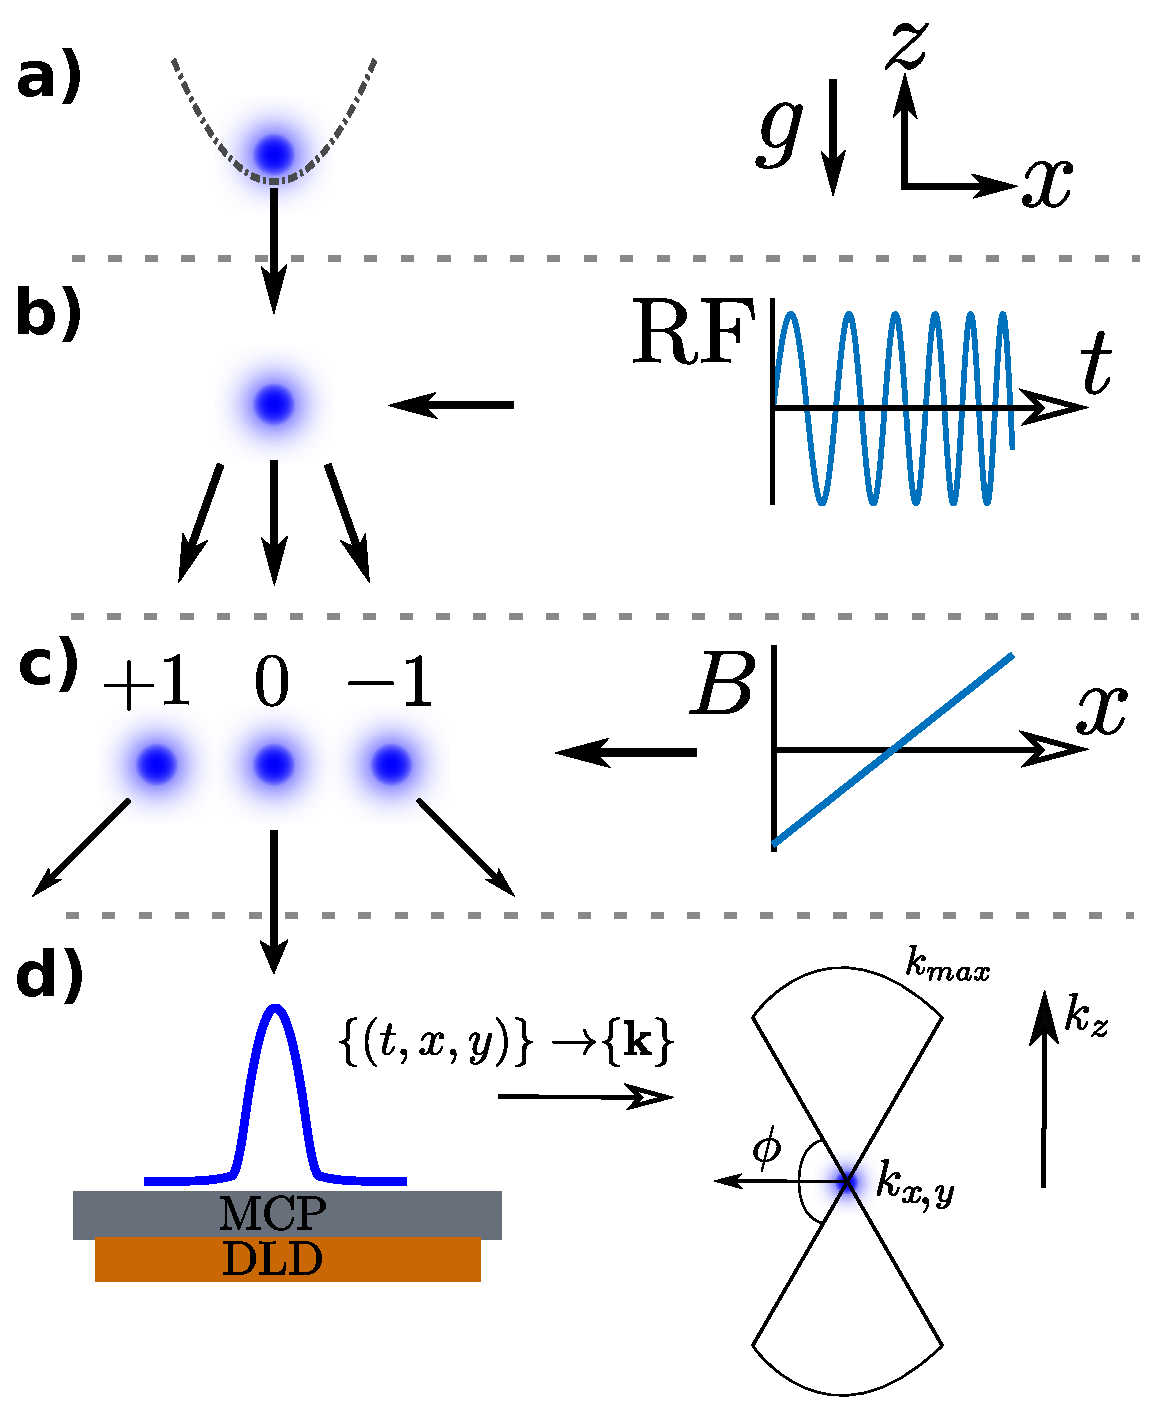
\includegraphics[width=\textwidth]{fig/QD/exp_cartoon.eps}
	    \end{minipage}
	\end{figure}

	


\subsection{Analysis of dilute tails} 
\label{sec:analysis}

  \begin{figure}
       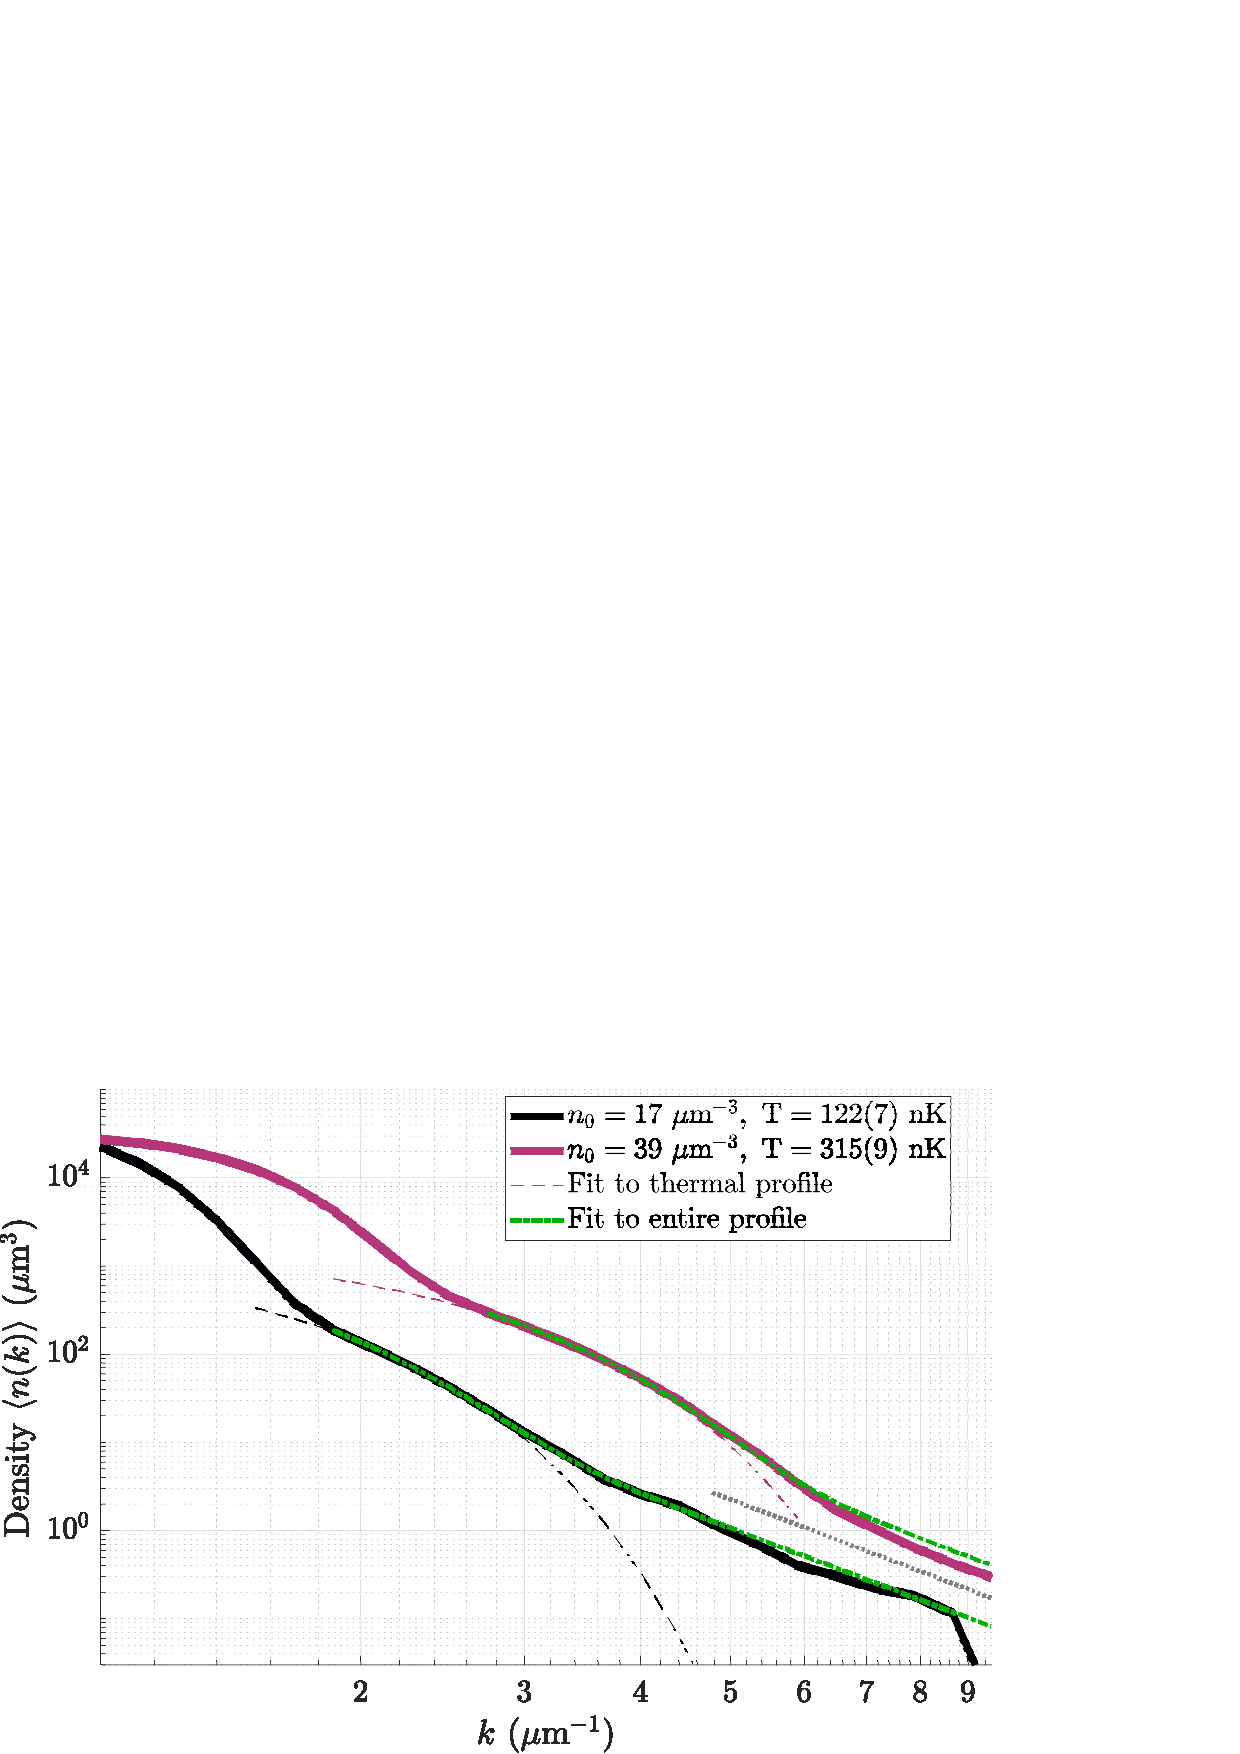
\includegraphics[width=\textwidth]{fig/QD/nk_density.pdf}
	        \caption{The empirical density of particle momenta in the far field from two trap configurations (black and magenta). Three regions are shown: At low $k$ the parabolic distribution of the BEC dominates. For larger $k$, the thermal parts (fits shown by dashed lines) decay super-exponentially as $e^{-k^2}$. For even larger $k$, these give way to the depletion region. A combined fit of the form $n_T(k) + C_4/k^4$ (green dot-dash lines) yields temperatures consistent with the thermal fit and also an amplitude $C_4$ of the depleted tail. The grey dotted line is a guide to the eye showing a $k^{-4}$ decay.}
	        \label{fig:empirical_density}
        \end{figure}	


	Fig. \ref{fig:empirical_density} shows the empirical density $n(k)$ for two data collection runs at the extreme values of $n_0$ used in the experiment\footnote{The spatial density of the atoms is given per cubic micron. The wavenumber $k$ has units $\micron^{-1}$, thus the particle density in $k$-space has units $(\micron^{-1})^{-3}=\micron^{3}$.}. The three regimes of the condensate, thermal depletion, and quantum depletion span over five orders of magnitude in density. The thermal part of the distribution is well fitted by the momentum distribution of an ideal Bose gas \cite{Dalfovo99}
	\begin{equation}
		\frac{n_T(k)}{{(2\pi)^3}} =\frac{N_T}{\zeta(3)} ~\left(\frac{\lambda_{dB}}{2\pi}\right)^3 g_{3/2}\left(\exp\left(-\frac{k^2 \lambda_{dB}^2}{4\pi}\right)\right)
		\label{eqn:th_fun}
	\end{equation}
	wherein the thermal de Broglie wavelength $\lambda_{dB} = \sqrt{2\pi\hbar^2/(m k_B T)}$ yields an estimate of the temperature $T$ which ranges from 100 to 320 nK in these experiments. Here, $g_{3/2}(\cdot)$ is the standard Bose integral, $\zeta(\cdot)$ is the Riemann zeta function, and $N_T$ is the number of atoms in the thermal component. The fits were made by manually selecting 
	Note that for a non-interacting gas in the thermodynamic limit, the {number of thermal atoms} %thermal fraction 
	is simply ${N_T^{\rm id}} = \zeta(3)(k_B T / \hbar\bar{\omega})^3{=\eta_T N}$, but for these condensates the critical temperature is reduced by $\approx20\%$ by interactions (see section \ref{sec:BEC_theory}).
	This, and the attendant twofold increase in the thermal fraction {$\eta_T$}  (relative to the non-interacting case), is accounted for by explicitly using $N_T$ as a fit parameter. 
	The thermal fits were applied to the $k$-interval that yielded the smallest mean-squared error, which generally excludes the condensate and also the high-momentum region where the thermal fraction makes a negligible contribution.
	The same lower bounds were used when fitting the combined thermal- and power-law functions (next section), but the upper bound was fixed at $k=10~\micron^{-1}$ for all cases.


	The thermal population decays super-exponentially with $k$, and hence cannot account for the counts we observe beyond $k\gtrsim 6~\micron^{-1}$. 
	In the rest of this section we present evidence in support of the identification of these counts with the quantum depletion. 
	First, though, I argue that the usual approach of a least-squares regression with a density function is unsuitable for the purpose of inferring power-law-like behaviour of the dilute tails, motivating the alternative approach presented in section \ref{sec:regression}.

\subsubsection{Difficulties with analysis of power laws}	
\label{sec:pow_issues}

	A standard approach would be to proceed with a routine fit of the $k$-space histogram with an additional term of the form $C_\alpha/k^\alpha$ to estimate the parameters of the purported quantum-depleted tail.
	However, fitting histograms with power laws is prone to return biased estimates of parameters and to drastically under-report uncertainties \cite{Clauset09,Virkar14}, especially when data is available over less than a couple of decades of dynamic range\footnote{As the authors of \cite{Clauset09} note, ``In practice, we can rarely, if ever, be certain that an observed quantity is drawn from a power-law distribution. The most we can say is that our observations are consistent with the hypothesis that $x$ is drawn from [...] a power law"}.
	In this section I demonstrate some of the problems with a least-squares regression using these measurements as a case study.
	Hereafter, $C_\alpha$ refers to a fit parameter, as distinct from the total contact $\mathcal{C}$ computed using the sweep theorem (Eqn. (\ref{eqn:sweep_theorem})), and $C_\textrm{sim}$ as determined from  numerical simulations. All three have dimensions m${}^{-1}$.


    \begin{figure}
       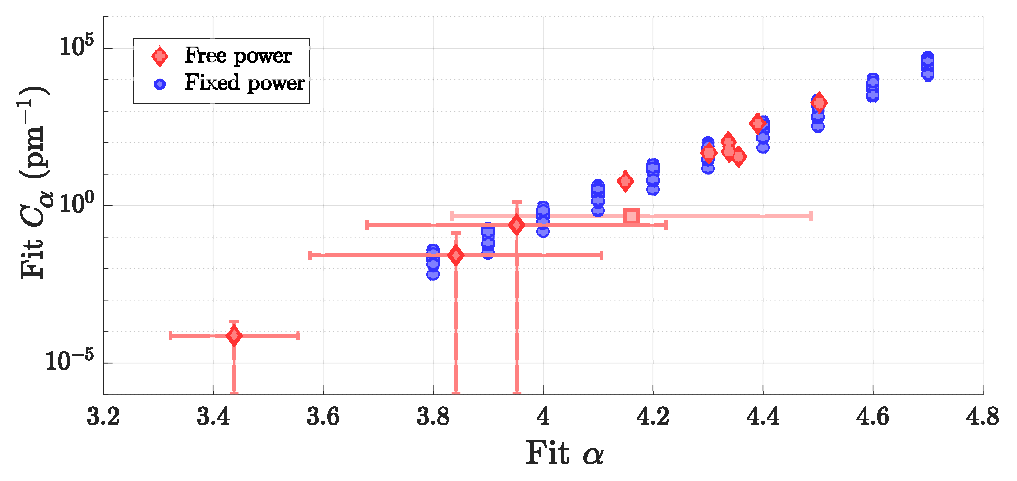
\includegraphics[width=\textwidth]{fig/QD/c_fit_problems}
	        \caption{Illustrating the large systematic errors in a fit to the density using a power law ansatz. If the fit to the density profiles (fig \ref{fig:empirical_density}) is replaced by $C_\alpha/k^\alpha$ and $\alpha$ used as a fit parameter it gives a wide variation in best-fit exponents and scale coefficients between each data set (red diamonds). The red square shows the mean fitted $\alpha$ and (geometric) mean $C_\alpha$ with standard deviation (in $\alpha$) shown as error bars. Blue circles show the amplitude coefficient $C_\alpha$ obtained from the same data sets with $\alpha$ fixed at values within the range of the free fit results. The choice of $\alpha$ strongly determines the coefficient $C_\alpha$, but the error bars (standard errors in fit parameters) are smaller than the markers in all cases. }
	        \label{fig:contact_determination_issues}
	\end{figure}

	
	If one augments the {thermal} fit function (Eqn. (\ref{eqn:th_fun})) with a power-law term and leaves $\alpha$ as a free parameter, the average exponent over all runs is 4.2(4). 
	For comparison, the prior work \cite{Chang16} reported power-law tails with an exponent 4.2(2).
	At first glance, one could simply determine the amplitude of the tails by fixing the exponent to 4 (being `within error' of the mean value), and thus find $C_{\alpha=4}$ which is, on average, 8(2) times greater than the coefficient predicted by Eqn. (\ref{eqn:pred_scaling}), and in general agreement with Ref. \cite{Chang16}.
	However, there are issues which undermine the utility of this otherwise standard approach.

	First, Fig. \ref{fig:contact_determination_issues} illustrates how the scale coefficient $C_\alpha$ depends exponentially on the choice of scaling exponent $\alpha$ when fitting to a fixed dataset.
	The red diamonds in Fig. \ref{fig:contact_determination_issues} (b) show the fit exponent and amplitude obtained from a fit (of the form ${n(k)} %$\hat{n}(k) 
	= n_T(k) + C_\alpha/k^\alpha$) to each data set, each representing a different BEC density. 
	The variation in the fit exponent is small (mean 4.2, standard deviation 0.4) but the corresponding variation in fit amplitude spans over six orders of magnitude.
	Although the mean $\alpha$ from the fits is only half a standard deviation (one standard-error interval) different from 4, the corresponding difference in amplitude $C$ varies by a factor of order 100.
	Therefore the decision of which value to take for the exponent is extremely consequential. 
	There is no justification for picking the adjusted value (4) over the mean value, especially given the point of contention is whether or not the tails are the depletion, which \emph{could} justify fixing the exponent.
	
	Moreover, fitting with a fixed exponent returns an unrealistic estimate of the systematic error associated with the fitting procedure.
	The blue circles in Fig. \ref{fig:contact_determination_issues} show the amplitudes returned from fits to all datasets when $\alpha$ is constrained at some specific value within about one standard deviation of the mean $\alpha$. 
	In this case, the variation in $C_\alpha$ is much reduced, down to a factor of about 10 between the extremes.
	However, $C_\alpha$ varies over about six orders of magnitude as $\alpha$ varies within the range of uncertainties reported here and in the prior work \cite{Chang16}. 
	A linear fit reveals that $d \log_{10} C_\alpha/d\alpha \approx 6.8$.
	These fits scarcely differ in their goodness-of-fit criterion (the mean square error) and so offer no obvious way to reconcile the expected distribution with these divergent  conclusions.
	The underlying issue here is that there is not enough data to accurately constrain $\alpha$, but assuming some fixed $\alpha$ effectively discards the large covariance between these parameters.
	Furthermore, this problem is not reflected in the error estimates in the fitting routines: The error bars representing the uncertainty in parameters from the fixed-$\alpha$ fits are smaller than the markers used in Fig. \ref{fig:contact_determination_issues}. 
		
	It is easy to see that a well-intentioned choice of $\alpha$, which is not statistically different from the best-fit estimates, can lead to a conclusion which either agrees perfectly or disagrees catastrophically with the predictions of Eqn. (\ref{eqn:pred_scaling}).
	In particular if one assumes that the data conforms to a power law with $\alpha=4$ (i.e. that the data conforms to the Tan-Bogoliubov theory), one arrives at a contradiction (that the coefficient $C_4$ does not conform to the theory) but the inherent uncertainty in this approach precludes the possibility of such a definitive statement.

	A deceptively reassuring result could be found by multiplying the empirical density by $k^4$ in the hope of observing a flat region, and identifying this with a $k^{-4}$ tail (see, for example, \cite{Makotyn14,Chang16}). %the quantum depletion. 
	The fitting procedure would be to appropriately scale the model of the thermal region (i.e. multiply Eqn. (\ref{eqn:th_fun}) by $k^4$) and add a constant term to fit the tail\footnote{Applying a fit of the form ${f_{\rm fit}(k)=}n_T(k)k^4+C$ to data scaled as ${f(k)} = k^4 n(k)$ minimizes the error term $\sum_i (k_{i}^{4}n(k_i)-k_{i}^4n_{fit}(k_i))$ which is equivalent to weighting the error terms {for the original $n(k)$ data} by $k^4$. 
	Moreover, the fit is highly sensitive to the choice of weighting function.
	If one constrains the exponent in the fit {of such an $f(k)$} at $\alpha=4$, then changing the {power of the} \emph{weighting function} of the squared errors in the fit from {$k^4$} by 0.1 {to $k^{4\pm0.1}$} changes the fitted {$C$} by a factor of ten.}.
	Unfortunately this offers no recourse from the issues described above and is not a definitive test for the presence of a power law or a way to obtain its parameters.
	Suppose the density actually decays as $n(k) \propto k^{-(\alpha+\delta)}$ with an exponent different by some $\delta$ from the expected value.
	Following the rescaling operation $n'(k) = k^\alpha n(k)$, one has a {function} %density 
	which would have the form $n'(k) \propto k^{-\delta}$. 
	Considering the range of $k$ examined in this (and the prior \cite{Chang16}) work, the scaled {function} %density 
	at the upper and lower end of the range would be predicted to differ by a factor $(k_\textrm{max}/k_\textrm{min})^\delta \approx 2^{0.1}\approx1.07$.
	This variation is dominated by the statistical fluctuations in the tails of the individual density profiles, and so would not be distinguishable by eye (or by fit) in a plot of the scaled density.
	
	The preceding discussion points to one of the primary challenges with power laws; the exponents are strongly entwined with the rate of occurrence of rare events, which by definition are subject to large statistical fluctuations and thus subvert even the most meticulous investigations.
	{Finally, the question of whether the data conforms to a power law at all is not amenable to a decisive conclusion. 
	For example, a log-normal distribution can produce similarly accurate predictions to the power law over finite regions \cite{Virkar14,Clauset09} even though there is no physical hypothesis that predicts such a distribution. 
	As I discuss in the next section, this underscores the challenge of identifying power-law behaviour in range-limited data, because even with these parameters the log-normal distribution eventually diverges from the power law, albeit over far a far larger domain than available in either Helium experiment.}

	To summarize, these problems with fitting power laws are ubiquitous, and made more difficult by the small range of $k$ which are visible in the helium experiments.
	In general, estimating the exponent of a purported power law is difficult and requires data spanning several orders of magnitude in scale \cite{Goldstein04,Clauset09,Virkar14,Hanel17}, which are not present in either {of the} helium experiment{s to date}.
	The preferred statistical tools for analysing power law distributions are maximum likelihood estimators, as discussed in Refs. \cite{Clauset09,Virkar14}.
	However, in these particle detection experiments the limited sampling region and presence of spurious detection events (see below) mean that such estimators are not appropriate.
	

	It is worth briefly recapitulating the motivation for fitting the present data with such care. A typical use of goodness-of-fit measures is to discern which of a collection of competing hypotheses provide a more accurate prediction of the phenomenon under study\footnote{This is an oversimplification - in fact, model parsimony and fit residuals are usually considered as well, either heuristically or thorugh, for instance, information criteria (such as the Bayes or Akaike criteria) and chi-squared tests, respectively.}. Typically these hypotheses are motivated by physical principles, and those based on different assumptions may make distinct predicitons. In this case, there are two questions we seek to answer. First, is there a signal beyond the BEC, thermal component, and background? Clearly, a fit including only these terms does not capture the slow decay observed in Fig. \ref{fig:empirical_density}. This alone is not sufficient to discard the hydrodynamic hypothesis, which would require answering a second and subtler question: Is the signal  consistent with the quantum depletion. In this respect, the fit-based parameter estimation does not provide substantial evidence in favour of the depletion-survival hypothesis - the fit results are manifestly not consistent with the relationship predicted by the Tan-Bogoliubov theory.

	In the next section I discuss an alternative approach which does not require -- and conversely cannot determine -- a precise value of the scaling exponent. 
	The approach discussed below permits a test of the Tan theory's validity in the far-field without assuming any specific properties of (and is clear about what can and cannot be said about) the actual form of the measured density distribution.
	
\subsubsection{Testing Tan's Tails}
\label{sec:regression}


	The prediction of the high-$k$ tail shape (via Eqn. (\ref{eqn:pred_scaling})) captures a great deal of information. 
	An important feature is that the amplitude of this tail is predicted to scale in proportion to the product $n_0 N_0$.
	One can integrate Eqn. (\ref{eqn:pred_scaling}) to predict the number of atoms in the trap whose wavevector has a modulus in the interval $k\in (k_\textrm{min}, k_\textrm{max})$. 

	\begin{equation}
		N_{k_\textrm{min},k_\textrm{max}} =\frac{\mathcal{C}}{2\pi^2}\left(\frac{1}{k_\textrm{min}}-\frac{1}{k_\textrm{max}}\right)
		\label{eqn:pred_num}
	\end{equation}
	For fixed $k_\textrm{min}$ and $k_\textrm{max}$, Eqn. (\ref{eqn:pred_num}) has the form {
	\begin{equation}
	N_{k_\textrm{min},k_\textrm{max}} = \Lambda N_0n_0
			\label{eqn:Lambda}
	\end{equation}
	}%
	(c.f. Eqn. \ref{eqn:pred_scaling} - note that the integral of $n(k)$ is most easily performed in spherical coordinates and requires the Jacobian $(2\pi)^{-3}d \kvec$ to ensure normalization.). 
	This form is directly testable by measuring the number of counts detected in the interval $(k_\textrm{min},k_\textrm{max})$ after producing a BEC of $N_0$ atoms with peak density $n_0$. 
	
	As above, $k_\textrm{min}$ was fixed at $6~\micron^{-1}$ which lies outside the thermal part for all the data sets (see Fig. \ref{fig:empirical_density}).
	However, the $k$-space field of view is restricted by the detector radius to $k\lesssim5\times 10^6$ m$^{-1}$ in the $(x,y)$ plane, which is only just sufficient to reach past the edge of the thermal region. 
	In the face of this tradeoff in the choice of $k_\textrm{max}$, I defined the bounds of the region of interest (ROI) by the minimum elevation angle $\phi_c=\pi/3$ rad above the $(x,y)$ plane and an upper bound of $k_\textrm{max} = 10~\micron^{-1}$.
	This amounts to an ROI consisting of two vertically oriented conical sections, each with half-angle $\pi/6$ from the $z$ axis, encompassing a total solid angle of $0.13\times 4\pi$ steradians. 
	The detector quantum efficiency of 0.08(2) and state-transfer efficiency of 25(2)\% combine  into the total efficiency $\epsilon\approx0.23(5)\%$.
	After discussing the results of this analysis, I will demonstrate their robustness against uncertainty in $\epsilon$ and the choices of $\phi_c$ and the $k$ bounds.

	A linear fit of the form $\hat{N}_{k_\textrm{min},k_\textrm{max}} = \Lambda_\textrm{fit} n_0 N_0 + \beta$ yields {an intercept} %a vertical intercept $c$ 
	consistent with zero ($\beta$=-0.9,  95\% confidence interval (CI) = (-3.1, 1.2)) and a good correlation ($r^2\approx0.8$), providing evidence supporting the expected linear relationship, and is shown in Fig. \ref{fig:exp_results}. 
	The fit has $p=1\times10^{-3}$ which indicates it is extremely unlikely that the results could be obtained from a null model (i.e. one where the measured counts are independent of the independent variable $N_0 n_0$)
	The correlation coefficient between the %(normalized) 
	variables {$N_{k_{\rm min},k_{\rm max}}$} %$N_\textrm{exp}$ 
	and $N_0n_0\propto(N_0^7\bar{\omega}^6)^{1/5}$ is 0.9.
	This is consistent with the claim that the product $N_0n_0$ is a predictor of the depleted population, which is consistent with Eqn. (\ref{eqn:pred_scaling}).
	No other physically-motivated combination of the independent variables provides a better fit.
	For comparison, a linear fit proves that the atom number {$N$} itself is a poor predictor of the detected number ($r^2=0.05~,p=0.54$), as is the density {$n_0$} alone ($r^2=0.4~,p=0.04$).

		\begin{figure}
	\begin{center}
		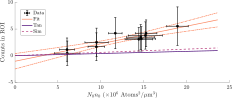
\includegraphics[width=\columnwidth]{fig/QD/regression_results}
			\caption{{Analysis of Tan's tails.} A linear fit shows that the product $N_0n_0$ is a good predictor of the number of counts within the region $(k_\textrm{min}=6~\micron^{-1},k_\textrm{max}~\micron^{-1})$, consistent with Eqn (\ref{eqn:pred_scaling}) 
			(solid orange line, dashed lines 95\% CI). The gradient {$\Lambda$} %$\Lambda_\textrm{fit}$ 
			{in Eqn. (\ref{eqn:Lambda})} can be predicted using Eqn (\ref{eqn:pred_scaling}) ({$\Lambda_{\rm pred}$} solid purple line) but this disagrees with the experiment by a factor of about 8. Our simulations (dashed line) show an increase in counts after release but by less than in the experiment. 
			}

		\label{fig:exp_results}
	\end{center}
	\end{figure}


	The gradient $\Lambda_\textrm{fit}$ is of particular interest because it can be predicted using Eqn. (\ref{eqn:pred_num}).
	Given an ROI, one can calculate $\Lambda_\textrm{pred} = 32\epsilon a^2(k_{\textrm{min}}^{-1}-k_{\textrm{max}}^{-1})/7$.
	The predicted slope disagrees with the empirical fit by a factor of $\Lambda_\textrm{fit}/\Lambda_\textrm{pred}= 8.3$, 95\% CI $(5.5,11)$.
	Figure \ref{fig:k_indep} shows that this conclusion holds regardless of the choice of $k$ boundary values: No matter the choice of $k_\textrm{min}$ or $k_\textrm{max}$, the resulting fit parameter $\Lambda_\textrm{fit}$ is 8(3) times larger than the Tan-Bogoliubov prediction. 

	However, while this method can accurately predict the number of detected atoms, it does not distinguish whether or not the data follows a power-law distribution, let alone a power-law with a particular exponent. 
	Consider these simple alternatives: that the tail amplitude is simply larger than expected (i.e. $n(k)=A\mathcal{C}/k^4$), or that the tail decay is somehow slower (i.e. $n(k)=\mathcal{C}/k^{4+\delta})$, or that it comes from another distribution altogether.
	Specifically, the density profiles $n(k)=A\mathcal{C}/k^4$ with $A=8(3)$ and $n(k)=\mathcal{C}/k^{\alpha}$ with $\alpha=3.86(2)$ both predict the variation of $\Lambda_{\rm pred}$ with $k_\textrm{min}$ and $k_\textrm{max}$ with comparable accuracy, as shown in Fig. \ref{fig:k_indep}. 
	Without the ability to precisely determine the exponent $\alpha$, or whether a power-law is present at all, there is insufficient evidence to conclude which of these is correct.
	Indeed, the predicted $k^{-4}$ behaviour is only a strict constraint inasmuch as the tails are \emph{known} to be the quantum depletion escaping the condensate without perturbation - which is itself the claim under test and as argued below is not necessarily expected.
	Fig. \ref{fig:k_indep} also shows, in red, predictions obtained by assuming log-normally distributed $k$ with parameters $(\mu,\sigma) \approx (1.235,0.95)$.
	The predictions are essentially identical over the ROI and so we can conclude only that the data is consistent with (a range of) power-law distributions, not that it \emph{is} drawn from a power law.

	\begin{figure}
	\begin{center}
		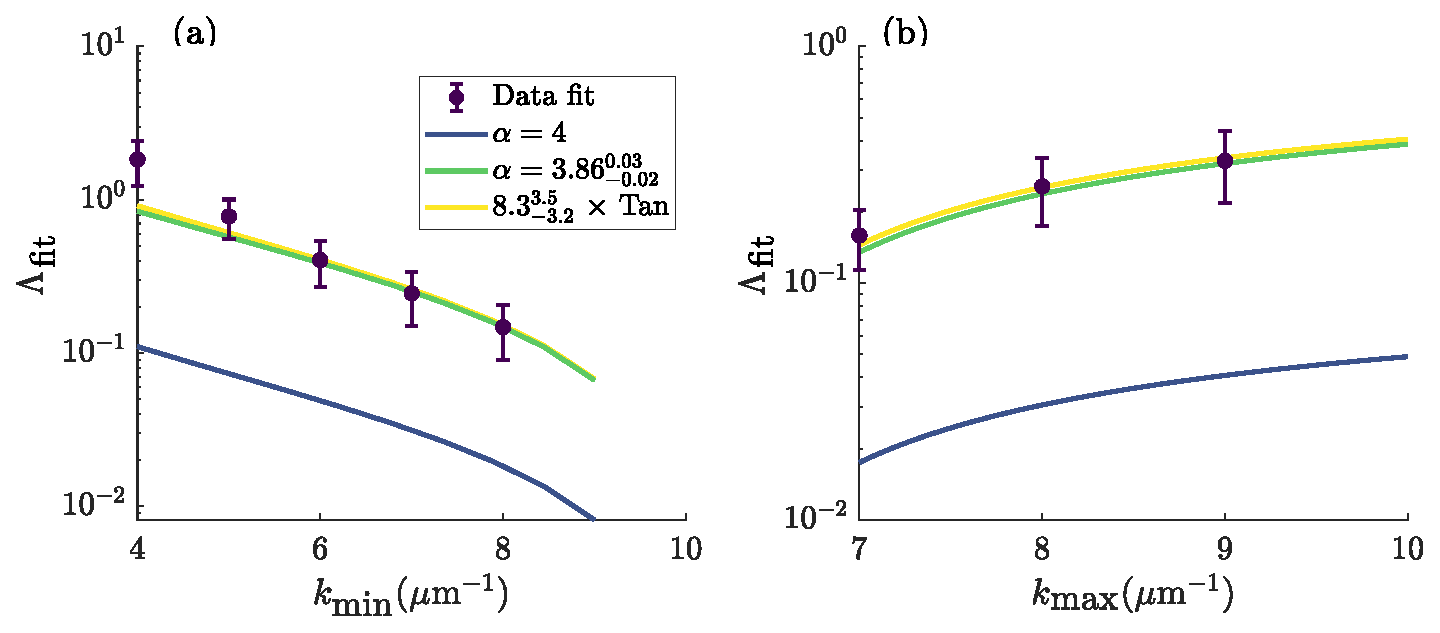
\includegraphics[width=\columnwidth]{fig/QD/k_indep}
			\caption{The experimental data {$\Lambda_{\rm fit}$} (points) show the $\Lambda_{\rm fit}$ to the entire data set with variable $k$ bounds ($k_\textrm{max}=10\micron^{-1}$ in (a) and $k_\textrm{min}=6\micron^{-1}$ in (b)).
		Predictions of $\Lambda$ based on Eqn (\ref{eqn:pred_scaling}) ({$\Lambda_{\rm pred}$}, blue), are shown along with the predictions {from Eqn. (\ref{eqn:Lambda}) using} a density function $n(k){=\mathcal{AC}/k^4}$ that {has an additional prefactor $\mathcal{A}=$8(3)} %times Eqn. (\ref{eqn:pred_scaling})
		(green) and one that has %exactly the amplitude $\mathcal{C}$ but 
		a modified exponent of {$\alpha=3.86(2)$ via $n(k)=\mathcal{C}/k^{\alpha}$} (yellow). 
		{A log-normal distribution produces nearly identical predictions (red, offset vertically for visibility).}
		The data does not distinguish between either of these hypotheses, and therefore provides limited information about {the prefactor $\mathcal{A}$ or exponent}% $C$ or
		$\alpha$.
		The error bars show the 95\% CI of the fit parameter $\Lambda_\textrm{fit}$, and parentheses enclose the uncertainty in the least-significant digit which is consistent with the 95\% CI.
			In (b), the deviation from the predictions at $k_\textrm{min}\lesssim6~\micron^{-1}$ is because the collection area starts to overlap with the thermal region.
			}
		\label{fig:k_indep}
	\end{center}
	\end{figure}


	We are then tasked with reconciling the nonlinear scaling of the detected counts, which is consistent with the quantum depletion, and the disagreement over the absolute number of detected counts.
	Ultimately, as I describe in the section \ref {sec:discussion}, the most prudent way through this dilemma is via alternative experimental designs.
	One conclusion remains robust: There are {almost} about ten times as many detections in the depletion region as one would expect based on the Tan theory {\emph{in situ}}. 
	Nonetheless, the particular nonlinear scaling of detected counts with the predictor $N_0n_0$ is concordant with the tails' originating in the quantum depletion.
	Furthermore, I describe below how the simulations indicate that the quantum depletion can survive the condensate expansion, presenting depleted tails in the far-field with modified amplitude. 
	We are therefore faced with the conclusion that tails are indeed a signature of quantum depletion, albeit subject to some effect during expansion into which the present analysis can see no further. 
	In order to find more insight into this observation, we performed numerical simulations of the time-dependent evolution of the expanding condensate, which I describe in the next section \ref{STAB}.
	In the next section I provide technical details of the experiments and rule out several systematic factors which could lead to this disagreement.
	% Our results could be seen as a count against the interpretation of these tails as a signature of the quantum depletion. 
	% However, we note two pieces of evidence that give weight to this interpretation. 
	% First, we are not aware of any other proposed physical effect which exhibits this specific nonlinear scaling relationship with respect to the atom number.
	% Second, we find evidence in our simulations (see below) that the momentum-space signature of the quantum depletion does survive the condensate expansion, and indeed appears in excess of the predicted \emph{in-situ} depletion.
 	
	


\subsection{Experimental details}
\label{sec:exp_details}
\subsubsection{Trap configuration}

	I prepared the BECs by evaporatively cooling helium in a harmonic magnetic trap with trap frequencies $\approx(45,425,425)$ Hz and a DC bias stabilized by our auxiliary field compensation coils \cite{Dall07,Dedman07}. For the tight trap, I increased the coil current after the cooling sequence to obtain trapping frequencies $\approx(71,902,895)$ Hz, ramping the current as a sigmoid step function to minimize in-trap oscillations. Note that the weak ($x$) axis of the trap is horizontal, with tight vertical confinement. The trap switched off with a $1/e$ time of $\approx38~\mu$s. The condensates then expanded for 2 ms before I transferred some of the initial $m_J=1$ condensate into the magnetically insensitive $m_J=0$ state via a Landau-Zener sweep to mitigate against distortion by stray magnetic fields during the free fall to the detector. The RF pulse was created by a function generator, amplified, and applied to the experiment chamber by a coiled antenna inserted into the BiQUIC coil housing. The pulse swept from 1.6-2.6 MHz over 1 ms and was centred on the resonance between the $m_J$ states. The determination of the transfer efficiencies $\eta_J$ for each of the $m_J$ states is discussed below. The sweep was $10^6$-fold wider than the RF width of the BEC which ensured uniform transfer at all momenta. Immediately after the RF sweep, the bias coils switched off and auxiliary push coils in the vertical (Z) and weak horizontal (X) axes are activated using a fast MOSFET switch to implement a Stern-Gerlach separation of the $m_J = -1,~0,$ and $+1$ pulses.

	The Roentdek DLD80 multichannel plate and delay-line detector stack, located 848mm below the trap, registers the arrival times and positions $(t_i,x_i,y_i)$ of each atom, indexed by $i$ \cite{Manning10}. 
	The velocity of each atom relative to the centre of mass of each cloud is calculated by $(v_x,v_y,v_z) = t_{i}^{-1}(x_i-\bar{x},y_i-\bar{y},\tfrac{1}{2}g_0(t_{cen}^2-t_{i}^{2}))$, where $g_0$ is the local gravitational acceleration, the overbar denotes the within-shot average and $t_{cen}$ is the time of flight of the centre of mass of the cloud. 
	The far-field momentum is thus obtained via $m\textbf{v} = \hbar\kvec$.
	The space and time resolution of the detector are 100 $\mu$m and 3 $\mu$s, respectively \cite{Henson18_BCR}, where the latter is comparable to a vertical resolution of $\approx 12~\mu$m.
	The detector efficiency of $8(2)\%$ was determined from analysis of the squeezing parameter of correlated atoms on the opposite sides of scattering halos \cite{Shin19,Shin20,Jaskula10}. 

	{The dominant uncertainty in the collection efficiency $\epsilon$ is the 25\% error in the detector quantum efficiency (QE), whereas the other factors (cutoff angle $\phi_c$ and transfer efficiency $\eta_0$) are more precisely known.
	Neither the uncertainty in the collection efficiency nor the choice of elevation angle cutoff $\phi_c$ have a significant effect on the findings. A change in quantum efficiency (QE) presents by changing the value of $\epsilon$ used in the prediction and also through the factor of $N_{0}^{7/5}$ used to compute the condensate density $n_0$. These effects partially cancel to produce a weak scaling of $\Lambda_\textrm{fit}/\Lambda_\textrm{pred}$ with respect to $\epsilon$.  Re-running the analysis using different QE yields fits that barely differ in the goodness-of-fit criterion and present comparable results for $\Lambda_\textrm{fit}$. The choice of collection area defined by the elevation angle cutoff $\phi_c$ has a weak effect on the result, but below statistical significance. 
	The relevant statistics are summarized in Table \ref{tab:choice_indep}.}

	\begin{table}
		\begin{minipage}{0.5\textwidth}
		\vspace{0cm}
		{\fontsize{11}{11}\selectfont
		\begin{tabular}{c c c c}
			\hline\hline

			QE & fit $r^2$ &  $\Lambda_\textrm{fit}$ & $\Lambda_\textrm{fit}/\Lambda_\textrm{pred}$\\      
			\hline
			0.05    &   0.83   &   0.2(0.1,0.3)  &  6.8(4.5,9.1)\\
			0.06    &   0.83   &   0.3(0.2,0.4)  &  7.4(4.9,9.8)\\
			0.07    &   0.83   &   0.3(0.2,0.4)  &  7.8(5.2,10.5)\\
			0.08    &   0.83   &   0.4(0.3,0.5)  &  8.3(5.5,11)\\
			0.09    &   0.83   &   0.5(0.3,0.6)  &  8.7(5.8,11.6)\\
			0.1     &   0.83   &   0.6(0.4,0.7)  &  9.0(6.0,12.1)\\
			0.11    &   0.83   &   0.6(0.4,0.8)  &  9.4(6.2,12.5)\\
			\hline
			$\phi_c$ & fit $r^2$ &  $\Lambda_\textrm{fit}$ & $\Lambda_\textrm{fit}/\Lambda_\textrm{pred}$\\
			\hline
			80$^\circ$    &   0.82   &   0.1(0.0,0.1) &  9.3(6.0,12.7)\\
			70$^\circ$    &   0.86   &   0.2(0.1,0.3) &  9.2(6.4,12)\\
			60$^\circ$    &   0.83   &   0.4(0.3,0.5) &  8.3(5.5,11)\\
			\hline\hline
		\end{tabular}
		}
		\end{minipage}
		\hfill
		\begin{minipage}{0.5\textwidth}
		\vspace{0cm}
		\caption{Sensitivity analysis for the systematic uncertainty in detector efficiency and choice of $\phi_c$. Terms in brackets are the upper and lower 95\% confidence intervals.}
		\label{tab:choice_indep}
		\end{minipage}
	\end{table}


\subsubsection{Peak density calibration}
\label{sec:n0_cal}

    The quantum depletion and contact are both predicted to depend solely on the condensed number and trapping frequencies via the condensate density, hence it is important to determine both quantities accurately. 
    % In the Thomas-Fermi approximation, the peak density of the condensate can be written as $n_0 = \mu/g$, where $\mu$ is the chemical potential, $g=4\pi\hbar^2a_{1,1}/m$ is the effective interaction strength, $m\approx6.6\times10^{-27}$ kg is the atomic mass, and $a=7.512$ nm is the s-wave scattering length between pairs of atoms in the $m_J=1$ state \cite{Moal06}. 
    The sole experimental parameters in the expression for the peak density (Eqn. (\ref{eqn:n0})) are the geometric trap frequency $\bar{\omega} = \left(\omega_x\cdot\omega_y\cdot\omega_z\right)^{1/3}$, and $N_0$, the number of atoms in the condensate. 
    The total atom number $N$ and trap frequency $\bar{\omega}$ can be determined simultaneously in a single shot using a pulsed atom laser, and the thermal fraction $\eta_T$ (section \ref{sec:th_spin}) thus determines the condensed number $N_0 = (1-\eta_T)N$. 

	The pulsed atom laser consists of a series of Fourier-broadened RF pulses centred on the minimum Zeeman splitting in the trap. 
	The pulse transfers atoms in the trap to the untrapped $m_J=0$ state with an approximately constant transfer rate across the cloud \cite{Manning10,Henson18_BCR}. 
	Approximately 2\% of the atoms are outcoupled per 100$~\mu$s pulse for $\approx$200 pulses, which eventually depletes the entire trap. 
	The atom laser thus prevents the detector from saturating and allows an accurate determination of the atom number, up to a factor of the quantum efficiency. 
	The trapping frequencies are determined by inducing centre-of-mass oscillations with a magnetic impulse, and finding the oscillation period from the atom laser pulses, detailed below.

	To illustrate how we obtain the trapping frequencies, consider an undamped harmonic oscillator in one dimension. The centre-of-mass momentum $p(t) = A \cos(2\pi f t))$ oscillates at a frequency $f$ Hz, and the centre of mass of a pulse outcoupled at time $t'$ lands on the detector at a position $x'(t+\tau) = p(t')\tau/m$, where $\tau$ is the time of flight of the centre of mass. Sampling the cloud motion with a sampling period T starting at initial time $t_0$ produces a series of pulses whose centres of mass land at $\{x_n = (A\tau/m) \cos(\omega(t_0+nT))\}$. The sampling frequency $f_s=1/T$ determines the \emph{Nyquist frequency} $f_N=f_s/2$, which is the maximum frequency that can be reconstructed unambiguously from such a sampling regime. When $f>f_N$ the signal manifests as a lower-frequency oscillation known as the \emph{alias} of the signal. The aliased frequency $f_a$ is

	\begin{equation}
	 f_a =
	  \begin{cases}
	   \frac{Z_N f_s}{2} - f & \text{if } Z_N \text{ even} \\
	   f - \frac{(Z_N-1)f_s}{2}       & \text{if } Z_N \text{ odd},
	  \end{cases}
	  \label{eqn:Z_N}
	\end{equation}
	
	where $Z_N = \lceil{f/f_N}\rceil$ is the Nyquist zone number, as described in numerous RF engineering references\footnote{Some good tutorials are presented \href{https://www.analog.com/media/en/training-seminars/tutorials/MT-002.pdf}{here} and \href{https://www.taborelec.com/Multi-Nyquist-Zones-Operation-Solution-Note}{here}. The trap frequency measurement technique specifically is presented in detail in \cite{Henson22_PAL}}. While it is not possible to determine $Z_N$ for a signal with an unknown (and not necessarily stationary) $f$ from samples taken at a fixed $f_s$, one can vary $f_s$ and determine both $Z_N$ and $f$.
	
	\begin{figure}
	\centering
		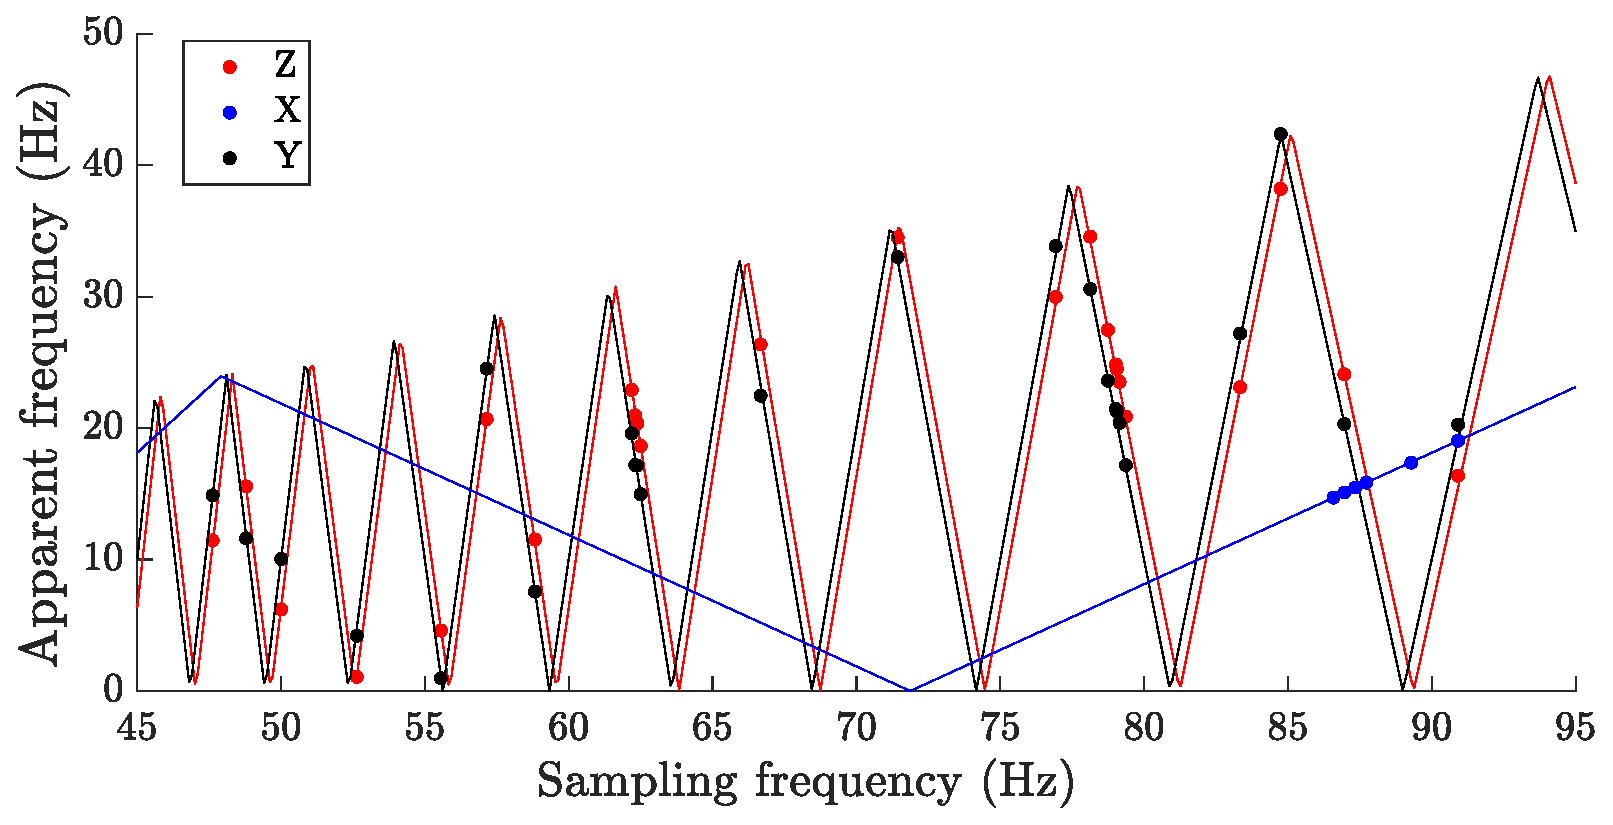
\includegraphics[width=0.7\textwidth]{fig/QD/sawtooth}
			\caption{Aliasing of the trap frequency oscillations under different sampling regimes. The sawtooth function is a one-parameter fit (Eqn. \ref{eqn:Z_N}) which determines the underlying frequency of the centre-of-mass oscillations.}
			\label{fig:sawtooth_plot}
	\end{figure}	

	Figure \ref{fig:sawtooth_plot} shows the \emph{apparent} frequencies of oscillation in each axis as a function of sampling frequency, as measured using the pulsed atom laser method described above.
	The maximum sampling frequency is limited by the temporal width of the BEC pulse landing on the detector. 
	We fit the apparent oscillation frequency in each axis with the one-parameter model Eqn. \ref{eqn:Z_N} and thus determine the characterisic frequencies of the magnetic trap.

	In fact, the measurements of $\omega_y$ and $\omega_z$ in Fig. \ref{fig:sawtooth_plot} use much more data than is strictly necessary to obtain $f$ unambiguously, and is presented to illustrate the technique. 
	One can obtain faster estimates by varying $f_s$ slightly and computing the gradient $df_a/df_s$ which unambiguously fixes $Z_n$ (assuming one does not accidentally cross a zone boundary, see eqn \ref{eqn:Z_N}).
	Therefore by selecting a sampling frequency near the middle of a known Nyquist zone, one can then obtain the Nyquist zone number with just a few measurements, as done in the $X$ axis (blue in Fig. \ref{fig:sawtooth_plot}). 
	
	For example, if the oscillations in the \(y\)-axis are determined to be in the 5\textsuperscript{th} Nyquist zone when sampling at 125~Hz, the corresponding correction to obtain the underlying frequency from the aliased frequency would be
	\begin{equation}
	    f_{\text{real}}=3 f_{\text{sampling}} + f_{\text{aliased}}.
	\end{equation}
	where \(f_{\text{real}}\) is the underlying frequency, \(f_{\text{aliased}}\) is the apparent frequency obtained from the fit, and \(f_{\text{sampling}}\) is the sampling frequency. 

	One can monitor changes in the underlying frequency $f$ with single measurements, which is especially relevant in the experiment of Chapter \ref{chap:tuneout} (again, assuming the shift is not great enough to push the signal into a different Nyquist zone\footnote{In Chapter \ref{chap:tuneout}, the 125Hz sampling rate means the zones are 62.5 Hz wide. The sub-Hz stability of the magnetic trap and the small perturbation from the probe beam ensure that the net oscillation frequency signal remains within a single Nyquist zone over the entire data collection campaign. }).	
	The final uncertainty in the trap frequency determination is simply the fit error as the Nyquist zone number is known exactly.


\subsubsection{Determining spin transfer efficiency}
\label{sec:th_spin}

	\begin{figure}
	\begin{center}
		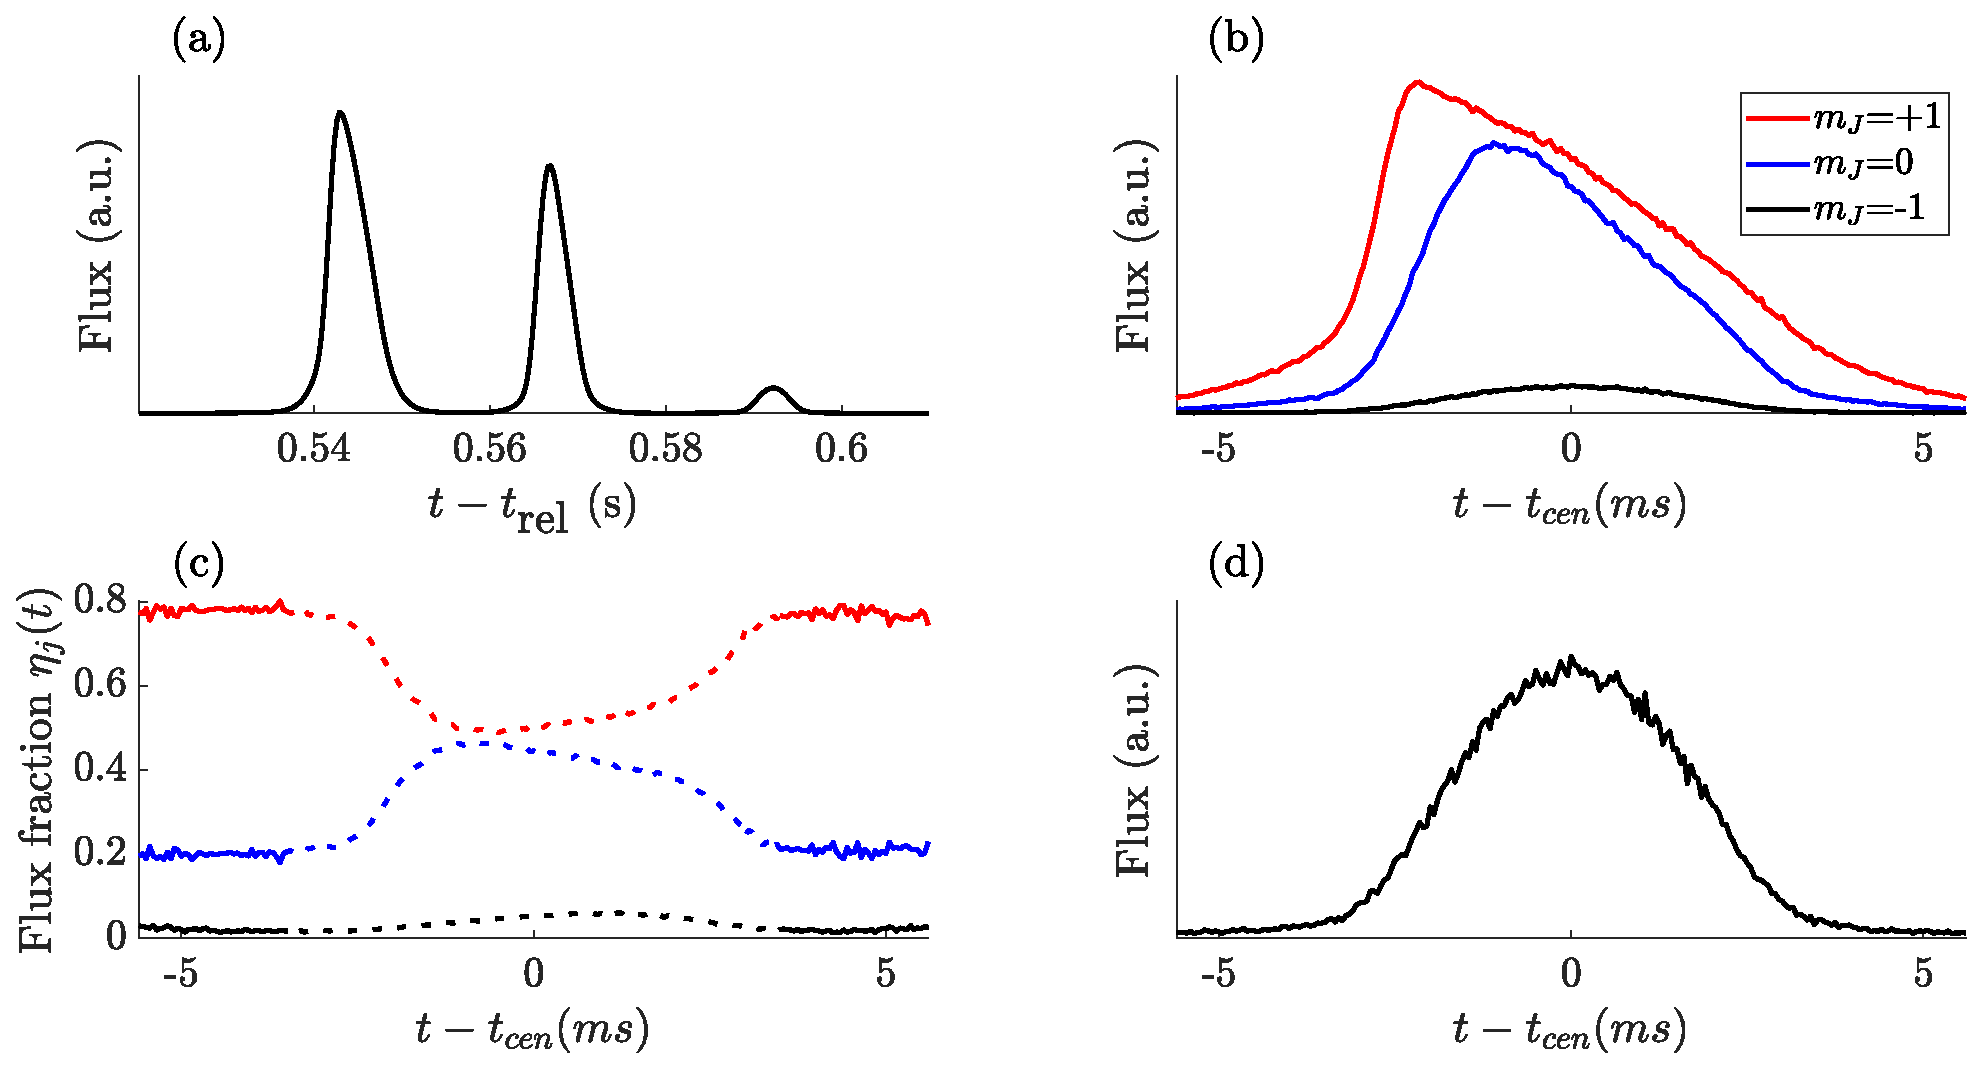
\includegraphics[width=\columnwidth]{fig/QD/frac_cal_profile.eps}
		\caption{Determining the RF transfer efficiency. The time-of-flight profiles of each pulse are resolved (a) by applying a weak Stern-Gerlach pulse during the time of flight. The pulses are aligned with respect to their centre-of-mass (b) and used to determine the pointwise fraction ((c), dotted line). Detector saturation is evident in the peaks (dashed lines), but not in the thermal tails (solid lines), which are used to compute the transfer efficiency. Because of its lower flux, the $m_J=-1$ pulse does not show any clear evidence of saturation (d) and is used to determine the thermal fraction and hence $N_0$.}
		\label{fig:frac_cal}
	\end{center}
	\end{figure}
	To calibrate the transfer efficiencies, a weaker Stern-Gerlach is used, such that each $m_J$ cloud hits detector at different times and positions, as illustrated in Fig. \ref{fig:frac_cal}. 
	The efficiencies $\eta_J$ cannot be calculated by counting the atoms in each cloud because the detector saturates during the peak condensate flux.
	However, the thermal parts are unsaturated and thus are comparable by aligning each cloud along the time (Z) axis.
	We can then compute the pointwise fraction of the atomic flux $\phi(t)$ accounted for by each cloud, $\eta_j(t) = \phi_j(t)/\sum_j\phi_j(t)$, as depicted in Fig. \ref{fig:frac_cal} (a-c).
	The ratio of densities between the clouds is roughly constant in the thermal part (Fig. \ref{fig:frac_cal} (c)), indicating the absence of saturation effects in the thermal part and a spin transfer efficiency that is independent of $k$. 
	The fraction of the original cloud transferred into each $m_J$ state is determined by taking the average $\langle\eta_j(t)\rangle$ over the thermal tails. 
	These efficiencies are approximately 74\%, 24\%, and 2\% in all runs for the $m_J=+1$, 0, and -1 states, respectively.
	While the $m_J=0$ and $m_J=1$ clouds clearly saturate the detector, the small fraction ($\approx2\%$) of the atoms transferred to the $m_J=-1$ state does not (Fig. \ref{fig:frac_cal} (d)). 
	A bimodal fit to the condensed and thermal parts, plus constant background, yields the thermal fraction $\eta_T$ and condensed fraction $1-\eta_T$.




\subsubsection{Noise sources}
\label{sec:spinpop}

	In early tests of the measurement sequence I noticed a contamination of the signal by spurious counts. 
	I identified these as remnant counts from the $m_J=+1$ cloud as they were still visible when we ran an experimental sequence without the Landau-Zener transfer. 
	This contamination appeared in a particular region of the detector image, and as such can be corrected for by subtracting their contribution from the counts collected during measurement shots. 
	While the cause of the cross-contamination is unclear, the count density outside the region of interest is similar in both the shots with the RF pulse and those without. 
	We could thus hypothesize that the remnant counts are atoms transferred into the $m_J=0$ state by non-ideal behaviour of the Stern-Gerlach pulses or magnetic field switches. 
	Note that only about one in a million atoms from the $m_J=1$ cloud are present in this manner in a given shot.
	{Such counts constitute about 10(5)\% of the detection events in the ROI. 
	The calibration without the Landau-Zener transfer enables a correction for their contribution by subtracting the counts measured in the calibration runs from the total used in Sec \ref{sec:regression}.
	However, because it is not possible to distinguish \emph{which} individual atoms are spurious and which are genuine quantum-depleted particles, the preferred power-law analysis (the maximum-likelihood estimator) is not available. 
	Basic MLEs are built assuming one has a sample of data drawn from a single category; the probabilistic combination of two indistinguishable categories of events falls outside the scope of this framework.}


	% \begin{table}
	% 		\begin{tabular}{ccccccc}
	% 		\hline \hline 
	% 		$n_0$ ($\mu$m$^{-3}$)  & $N_0\times10^{-5}$ & $\eta_\textrm{Th}$ & T (nK) & $N_\textrm{det}$ & $N_\textrm{pred}$ & $N_\textrm{det}/N_\textrm{pred}$ \\ 
	% 		\hline 
	% 		17(2) & 3.6(3) & 0.09 & 130(20) & 1.2(1) & 0.3(1) & 5(2) \\ 
	% 		17(3) & 3.6(6) & 0.08 & 190(20) & 0.3(04) & 0.3(1) & 1(1) \\ 
	% 		19(1) & 5.1(3) & 0.18 & 150(10) & 1.9(1) & 0.3(1) & 6(3) \\ 
	% 		19(2) & 4.9(5) & 0.09 & 150(10) & 2.8(1) & 0.4(1) & 7(4) \\ 
	% 		20(1) & 5.7(2) & 0.1  & 137(9)  & 5.0(1) & 0.5(1) & 10(4) \\ 
	% 		39(4) & 3.8(3) & 0.11 & 252(3)  & 3.7(1) & 0.6(1) & 6(4) \\ 
	% 		39(4) & 3.9(3) & 0.11 & 268(2)  & 4.4(1) & 0.6(1) & 8(5) \\ 
	% 		39(3) & 3.8(3) & 0.1  & 249(3)  & 4.1(1) & 0.5(1) & 8(4) \\ 
	% 		39(3) & 3.7(3) & 0.09 & 237(3)  & 3.6(1) & 0.5(1) & 7(4) \\ 
	% 		39(3) & 4.0(2) & 0.14 & 312(3)  & 4.9(1) & 0.5(1) & 10(5) \\ 
	% 		41(2) & 4.6(2) & 0.12 & 302(3)  & 6.6(2) & 0.7(2) & 10(6) \\ 
	% 		\hline \hline s
	% 		\end{tabular}
	% 		\caption{Summary of results for each data run. The peak density is determined from measurements of the trapping frequencies and the condensed number (via $N_0=N_\textrm{tot}(1-\eta_\textrm{Th})$, using the total number $N_\textrm{tot}$ and thermal fraction $\eta_\textrm{Th}$). The number $N_\textrm{Detect}$ of atoms detected in the region of interest (results shown here for the largest ROI) can be compared to the predictions of the Tan theory, as in the main text.}
	% 		\label{tab:run_results}
	% 	\end{table}






\section{Numerical simulations}
\label{STAB}

	The measurements described above are complemented by numerical simulations\footnote{ The simulations were run by my collaborator P. Deuar and their methods are detailed in \cite{Ross21}.} of the dynamics of the momentum distribution after the trap release using a Stochastic Time-Adaptive Bogoliubov (STAB) method in the positive-P framework  \cite{Deuar11,Kheruntsyan12}. 
	These show that the non-adiabatic release of the trap is responsible for survival of the depletion, and that the depleted particles acquire additional kinetic energy from the mean-field energy of the condensate during the subsequent adiabatic expansion. 
	These factors result in an amplification of the momentum tails relative to the in situ values {by a factor of up to about two}, and are not captured in the hydrodynamic approximation. 
	However, there remains a quantitative disagreement between simulation and the experiment {in that the experimental tails are even heavier by a large margin.}

	\begin{figure}
	        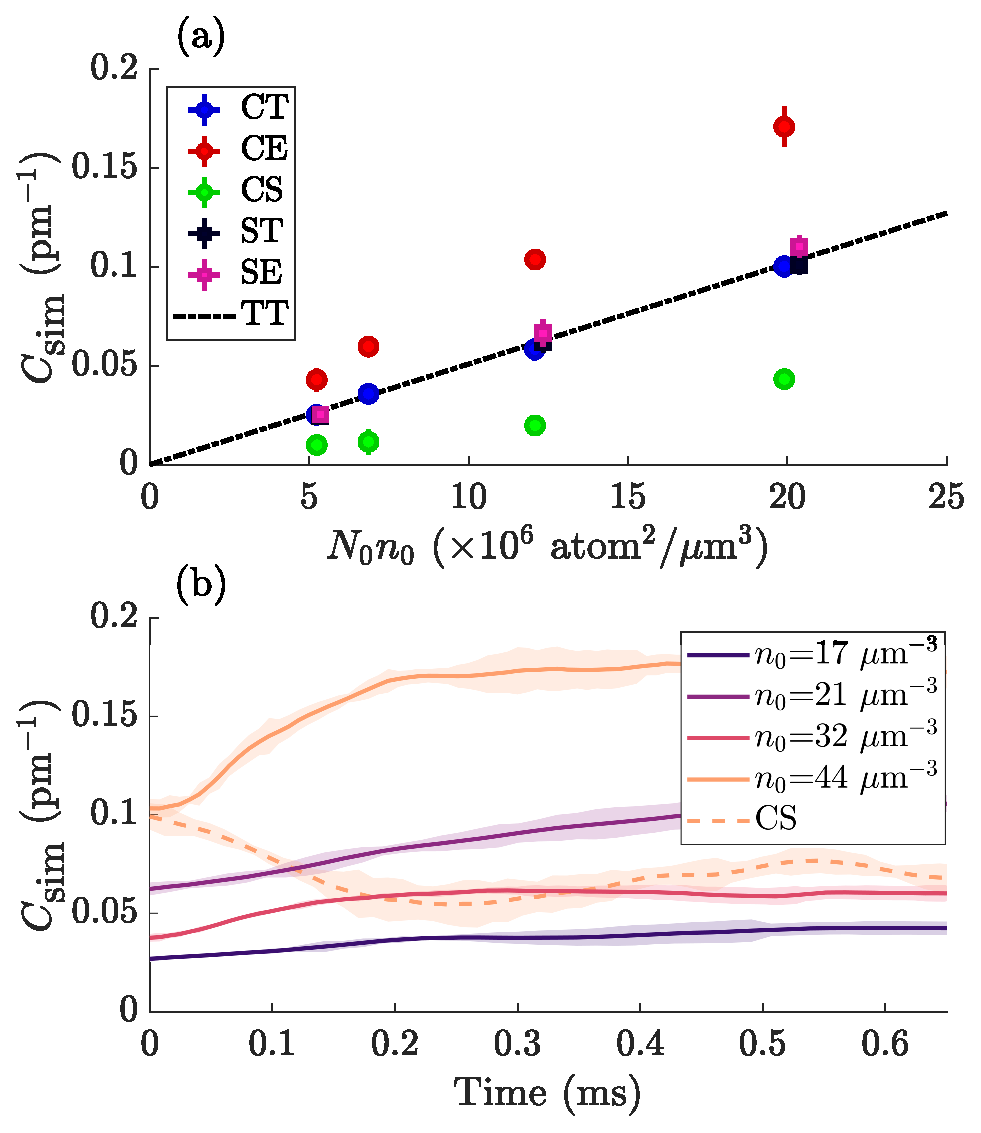
\includegraphics[width=\columnwidth]{fig/QD/sim_results.eps}
	        \caption{Simulations of release from the trap. (a) Steady-state values of the simulated contact. Simulations of condensates released from a cigar-shaped trap (CT) are consistent with the Tan theory (TT) before release, and show an increase in contact after the trap release (CE). A slow relaxation of the transverse trapping frequencies (CS) shows a decrease in line with the predicted value of the lower density. Spherical traps (ST,SE) lack any directions of tight confinement, wherein a longer interaction time prevents the escape of depleted particles as seen in cigar traps. (b) the time-dependence of the contact stabilizes after a time on the order of $1/\omega_x$, several hundred $\mu$s. The expanded contact is consistently about 1.7 times the Tan theory. For comparison, the experimental control pulses are implemented after 2 ms of expansion. When the transverse trapping frequencies are slowly reduced by half (dotted line), the in-situ contact relaxes.}
	        \label{fig:sim_fig}
	\end{figure}
	
	The simulations started from a cigar-shaped trap with parameters matched to the experimental conditions. 
	The in-trap state before release from the trap at time $t=0$ (marked CT in Fig. \ref{fig:sim_fig} (a)) was consistent with the adiabatic sweep theorem. 
	Following expansion from the cigar trap, the simulated tail amplitude increased and stabilized within a few hundred microseconds (CE in Fig. \ref{fig:sim_fig} (a)), much sooner than the 2 ms delay between the trap release and application of the rf and Stern-Gerlach pulses. 
	Fig. \ref{fig:sim_fig}~(b) shows the time evolution of the tail amplitude {$C_{\rm sim}$ extracted from a $n(k)=C_{\rm sim}/k^4$ fit to the simulated density} %for the simulated traps 
	using {an ROI with the same cutoff elevation angle $\phi_c=\pi/3$ as in the experiment.}  
	In this configuration the steady-state value of the momentum tails was a factor of 1.64(9) above the predictions of Eqn. (\ref{eqn:pred_scaling}). 
	{An analysis of the occupation of the tails according to (\ref{eqn:pred_num}), gives very similar factors $\mathcal{A}_{\rm sim}$ for the increase in the strength of the tails (relative to \emph{in-situ} predictions) during evolution, as shown in Table~\ref{tab:Nminmax}.}

	\begin{table}

	\begin{minipage}{0.5\textwidth}
	\vspace{0pt}
	%\renewcommand{\arraystretch}{0.1}
	\setlength{\tabcolsep}{0.5pt}
	{\fontsize{8}{11}\selectfont
	\begin{tabular}{c|ccc|c|c}
	\hline\hline
	$n_oN$	&$k_{\rm min}$&$k_{\rm max}$ & $\phi_c$ & $N_{k_{\rm min},k_{\rm max}}$	&ratio $\mathcal{A}_{\rm sim}$ 	\\
	($10^6\mu$m${}^{-3}$)& \multicolumn{2}{c|}{($\mu$m${}^{-1}$)}& (deg) &final& 	final/in situ\\
	\hline
	\multicolumn{6}{l}{Rapid release from trap (CE)}\\
	5.237(16)   & 2.0 & 3.5 & 60 & 193(8)    & 1.38(5)\\
	12.09(6)    & 2.25 & 3.5 & 60 & 362(10)   & 1.43(4)\\
    6.86(3)     & 2.75 & 4.0 & 60 & 163(4)   & 1.45(4)\\
    19.90(8)    & 3.0 & 4.0 & \ \ 40 & \ \ 423(8)    & \ \ \ 1.37(3) \\
    19.90(8)    & 3.0 & 4.0 & \ \ 50 & \ \ 408(8)    & \ \ \ 1.56(3) \\
    19.90(8)    & 3.0 & 4.0 & 60 & 368(7)    & 1.80(4) \\
    19.90(8)    & 3.0 & 4.0 & \ \ 70 & \ \ 282(6)    & \ \ \ 2.00(4) \\
    19.90(8)    & 3.0 & 4.0 & \ \ 80 & \ \ 157(5)    & \ \ \ 2.19(6) \\
	\hline
	\multicolumn{6}{l}{Rapid release, spherical (SE)}\\
	5.35(2)     & 2.0 & 3.25 & 60 & 120(9)    & 0.92(6)\\
	12.23(6)    & 2.0 & 3.0 & 60 & 256(11)   & 1.05(4)\\
    20.38(10)   & 3.0 & 4.0 & 60 & 232(10)    & 1.10(5) \\
	\hline
	\multicolumn{6}{l}{Slow ramp down of trap (CS)}\\
	5.237(16)   & 2.0 & 3.5 & 60 & 55(10)   & 0.37(6)\\
	12.09(6)    & 2.0 & 3.5 & 60 & 103(21)   & 0.31(5)\\
	6.86(3)     & 2.5 & 4.0 & 60 & 50(8)   & 0.34(6)\\   
	19.90(0)    & 2.5 & 4.0 & 60 & 181(14)   & 0.54(4)\\
	\hline\hline
	\end{tabular}
	}%fontsize
	\end{minipage}
	\hfill
	\begin{minipage}{0.5\textwidth}
	\vspace{0pt}
	\caption{
	Tail strength data in simulations, referenced by the value of $n_0N$. $N_{k_{\rm min},k_{\rm max}}$ is calculated as per (\ref{eqn:pred_num}). The ratio $\mathcal{A}_{\rm sim}$ of tail strength  in the expanded cloud compared to Tan theory predictions is obtained by dividing $N_{k_{\rm min},k_{\rm max}}$  at the final time by its value in situ at $t=0$. $k_{\rm max}$ is chosen to still contain all $4\pi$ steradians inside the square lattice, while  $k_{\rm min}$ to avoid overlap with the expanding condensate.
	}
	\label{tab:Nminmax}
	\end{minipage}
	\end{table}

	To understand the disagreement with earlier theory \cite{Qu16}, which predicted no depletion survival, we also investigated the effect of adiabatic expansion on the in-trap depletion by simulating a slow decrease of the transverse trapping frequencies by a factor of two (CS), and found that the in-trap contact {$C_{\rm sim}$ as well as the the tail strength $N_{k_{\rm min},k_{\rm max}}$ from (\ref{eqn:pred_num})} 
	decreased roughly as predicted by Eqn. (\ref{eqn:pred_scaling}) in these instances --- see the dashed line in Fig.~\ref{fig:sim_fig} (b) {and Table~\ref{tab:Nminmax}.} 
	We also found that the relative factors between Eqn. (\ref{eqn:pred_num}) and the simulated tails (i.e. $C_\textrm{sim}/\mathcal{C}$ {and $\mathcal{A}_{\rm sim}$) depend} on choice of cutoff angle $\phi_c$. 
	% Put another way, the momentum distribution in the simulations is anisotropic and takes the form $f(\theta,\phi)/k^4$ - note that the average of an angle-dependent power law decay preserves the power-law behaviour.
	{We find that apparent tail strengths $C_\textrm{sim}$ {and $\mathcal{A}_\textrm{sim}$ are} larger for smaller collection regions that are more tightly concentrated about the %vertical 
	strong trapping axis, whereas larger collection angles (that include areas closer to the weak axis) produce lower apparent tail strengths. 
	{Data on $\mathcal{A}_{\rm sim}$ are shown in Table~\ref{tab:Nminmax} while 
	$C_\textrm{sim}$ was 1.6(1), 1.9(2), and 2.2(3) times $\mathcal{C}$ for $\phi_c$ values of 60, 70, and 80 degrees, respectively.}
	We note that the experimental results (Tab. \ref{tab:choice_indep}) could be said to display a similar trend, but the result is not statistically significant.
	Details regarding the implementation of the simulations can be found in \cite{Ross21}.


% \begin{table}
% \blu{
% 	\begin{center}
% 	%\renewcommand{\arraystretch}{0.1}
% 	\setlength{\tabcolsep}{0.5pt}
% 	{\fontsize{8}{11}\selectfont
% 	\begin{tabular}{c|ccc|c|c}
% 	\hline\hline
% 	$n_oN$	&$k_{\rm min}$&$k_{\rm max}$ & $\phi_c$ & $N_{k_{\rm min},k_{\rm max}}$	&ratio $\mathcal{A}_{\rm sim}$ 	\\
% 	($10^6\mu$m${}^{-3}$)& \multicolumn{2}{c|}{($\mu$m${}^{-1}$)}& (deg) &final& 	final/in situ\\
% 	\hline
% 	\multicolumn{6}{l}{Rapid release from trap (CE)}\\
% 	5.237(16)   & 2.0 & 3.5 & 60 & 193(8)    & 1.38(5)\\
% 	12.09(6)    & 2.25 & 3.5 & 60 & 362(10)   & 1.43(4)\\
%     6.86(3)     & 2.75 & 4.0 & 60 & 163(4)   & 1.45(4)\\
%     19.90(8)    & 3.0 & 4.0 & \ \ 40 & \ \ 423(8)    & \ \ \ 1.37(3) \\
%     19.90(8)    & 3.0 & 4.0 & \ \ 50 & \ \ 408(8)    & \ \ \ 1.56(3) \\
%     19.90(8)    & 3.0 & 4.0 & 60 & 368(7)    & 1.80(4) \\
%     19.90(8)    & 3.0 & 4.0 & \ \ 70 & \ \ 282(6)    & \ \ \ 2.00(4) \\
%     19.90(8)    & 3.0 & 4.0 & \ \ 80 & \ \ 157(5)    & \ \ \ 2.19(6) \\
% 	\hline
% 	\multicolumn{6}{l}{Rapid release, spherical (SE)}\\
% 	5.35(2)     & 2.0 & 3.25 & 60 & 120(9)    & 0.92(6)\\
% 	12.23(6)    & 2.0 & 3.0 & 60 & 256(11)   & 1.05(4)\\
%     20.38(10)   & 3.0 & 4.0 & 60 & 232(10)    & 1.10(5) \\
% 	\hline
% 	\multicolumn{6}{l}{Slow ramp down of trap (CS)}\\
% 	5.237(16)   & 2.0 & 3.5 & 60 & 55(10)   & 0.37(6)\\
% 	12.09(6)    & 2.0 & 3.5 & 60 & 103(21)   & 0.31(5)\\
% 	6.86(3)     & 2.5 & 4.0 & 60 & 50(8)   & 0.34(6)\\   
% 	19.90(0)    & 2.5 & 4.0 & 60 & 181(14)   & 0.54(4)\\
% 	\hline\hline
% 	\end{tabular}
% 	}%fontsize
% 	\end{center}
% 	\caption{
% 	Tail strength data in simulations. Based on final times in the simulations described in Table~\ref{tab:simdata}, referenced by the value of $n_0N$. $N_{k_{\rm min},k_{\rm max}}$ is calculated as per (\ref{eqn:pred_num}). The ratio $\mathcal{A}_{\rm sim}$ of tail strength  in the expanded cloud compared to Tan theory predictions is obtained by dividing $N_{k_{\rm min},k_{\rm max}}$  at the final time by its value in situ at $t=0$. $k_{\rm max}$ is chosen to still contain all $4\pi$ steradians inside the square lattice, while  $k_{\rm min}$ to avoid overlap with the expanding condensate.
% 	\label{tab:Nminmax}}
% 	}
% \end{table}


%\org{NOTE: orange text are just explanatory notes for us that should be removed in the final cut.}


\section{Discussion}
\label{sec:discussion}

	
	

	% In sum, the number of atoms in the large-$k$ tails is predicted by the product $N_0n_0\propto(N_{0}^7\bar{\omega}^6)^{1/5}$, in line with Tan's theory of the contact (Eqns. \ref{eqn:pred_scaling},\ref{eqn:pred_num}). 
	% However, the sensitivity of this relationship is significantly different than expected by a factor of order 8(3), which is not accounted for by any known systematic effects.
	% As discussed in section \ref{sec:analysis}, there are fundamental challenges in the analysis of heavy-tailed distributions which preclude any decisive evidence regarding the functional form of the momentum tails.
	% The evidence suggests that the tails are indeed a signature of quantum depletion (per the first point), albeit subject to some physical effect during the expansion as discussed below, {or some nonequilibrium enhancement in the trapped state}.
	% Note that the prior work \cite{Chang16} reported results which fall within the uncertainty range of our analysis.
	% Indeed, Fig. 4 in \cite{Chang16} could be said to display the relevant scaling with respect to $N_0n_0$, but the reported values of the apparent contact should be considered alongside the caveats discussed in Section \ref{sec:pow_issues}.
	
	% Taken together with the simulations, these findings show that the survival of the quantum depletion into the far-field is plausible, but not as a straightforward mapping into the far-field density.
	% In a non-interacting ballistic expansion, the far-field density distribution would be a direct realization of the in-trap momentum distribution of the cloud. 
	% However, this correspondence is known not to be completely faithful because the dispersal of the mean-field energy into kinetic energy, known as the release energy, imparts some acceleration to the atoms during the early stages of the expansion. 
	% This effect is responsible for the famous inversion of the cloud aspect ratio upon release from harmonic traps. 

	% One potential interpretation of these results is that the depleted atoms are accelerated by the non-uniform mean-field energy of the condensate during the expansion.
	% In detail, after a quench into the free particle regime, the condensate expands hydrodynamically on timescales of $1/\omega$. 
	% This is an adiabatic process for the low momentum depletion, whereby some depleted atoms are absorbed back into the condensate in agreement with \cite{Qu16}.
	% However, the characteristic time for reabsorption is $\hbar/gn_0$, slow enough that quasiparticles in the particle branch of the Bogoliubov dispersion have sufficient velocity to escape the expanding cloud without being reabsorbed and thus transition to free atoms. 
	% Quasiparticles whose wavenumber exceeds that of the speed of sound lie within the particle-like branch of the Bogoliubov spectrum, which for our considerations is on the order of $k\gtrsim2~\micron^{-1}$, well within the thermal velocities. Therefore most atoms with $k\gtrsim 6 \micron^{-1}$ would avoid absorption.
	% This effect leads to the persistence of populated high-$k$ modes in the far-field, which were detected in the experiment.

	% Moreover, an atom inside the BEC experiences an effective force from the gradient of the mean-field potential $\textbf{F} = -4\pi\hbar^2 m^{-1}a \nabla  n(x)$. 
	% This endows escaping depleted particles with a greater momentum, increasing the amplitude of the tails in the far-field. 
	% Further, it is much easier for depletion atoms to escape and be accelerated along the tightly-confined axes of a cigar-shaped cloud because the distances $R_{TF}=\frac{1}{\omega}\sqrt{2gn_0/m}$ are reduced by $\bar{\omega}/\omega_{y,z}$, whereas the initial mean depletion velocities \textit{in situ} $v\sim \sqrt{2gn_0/m}$ are isotropic.
	% Indeed, spherical clouds (SE) exhibit a much weaker effect than the elongated clouds (CE) owing to the longer escape time.
	% This also presents as an increase in $C_\textrm{sim}$ {and $\mathcal{A}_{\rm sim}$ for} collection regions {with a higher $\phi_c$}. 
	% The statistical uncertainty in the experimental findings preclude a definitive comparison on this particular point.
	% % This effect is exacerbated in light atoms like $^{4}$He, whereas it would be suppressed by a $\sim500$-fold in $^{87}$Rb experiments \cite{Makotyn14} because the acceleration scales with $1/m^2$. 

	% The interpretation just described is supported by another observation within the simulations:
	% During the expansion, the total number of depleted particles decreases (reabsorption) simultaneously with an increase of the large-k population (forcing). 
	% This {also corroborates the above interpretation} %constitutes a partial explanation 
	% of the experimental findings, and results in tail amplitudes which are consistent with the quantum depletion multiplied by a constant factor. 
	% However, a mystery remains: Why is there an excess of particles in the depletion region which is so much greater than accounted for by this picture? 
	% This issue should be resolved if far-field observations are to be interpreted in terms of the in-trap physics of interest. 
	
	% As discussed, the systematic uncertainties are unable to account for the observed excess population of the quantum-depleted tails.
	% Futher, despite the ultracold clouds being realized at finite temperatures, the thermal population of quasiparticles cannot account for the observed counts. 
	% The thermal quasiparticles in the Bogoliubov picture simply map onto the thermal population of constituent particles of the same momentum \footnote{See, for example, \cite{PethickSmith} Chap. 8.3. or \cite{Vogels02}}. 
	% {Therefore the phonon/particle changeover is not responsible for the inflections seen at high $k$ in Fig.~\ref{fig:contact_determination_issues}(a).} 
	% Hence, given the doubly-exponential decay of thermally populated states, the large-$k$ tails are unambiguously \emph{not} thermal effects. 

	% The utility and ubiquity of far-field imaging (including in MCP-DLD setups using helium) stems from the relative simplicity of implementation and interpretation.
	% A systematic deviation from the expected \emph{in-situ} amplitude of the high-$k$ tails could mean that such techniques are not the appropriate tool to study the details of the quantum-depleted momentum distribution.

\subsection{Summary of results}

    One potential interpretation of these results is that the depleted atoms are accelerated by the non-uniform mean-field energy of the condensate during the expansion.
	In detail, after a quench into the free particle regime, the condensate expands hydrodynamically on timescales of $1/\omega$. 
	This is an adiabatic process for the low momentum depletion, whereby some depleted atoms are absorbed back into the condensate in agreement with \cite{Qu16}.
	However, the characteristic time for reabsorption is $\hbar/gn_0$, slow enough that quasiparticles in the particle branch of the Bogoliubov dispersion have sufficient velocity to escape the expanding cloud without being reabsorbed and thus transition to free atoms. 
	Quasiparticles whose wavenumber exceeds that of the speed of sound lie within the particle-like branch of the Bogoliubov spectrum, which for our considerations is on the order of $k\gtrsim2~\micron^{-1}$, well within the thermal velocities. Therefore most atoms with $k\gtrsim 6 \micron^{-1}$ would avoid absorption.
	
	Moreover, an atom inside the BEC experiences an effective force from the gradient of the mean-field potential $\textbf{F} = -4\pi\hbar^2 m^{-1}a \nabla  n(x)$. 
	This endows escaping depleted particles with a greater momentum, increasing the amplitude of the tails in the far-field, and has been observed for the thermal part of the cloud in other experiments \cite{Ozeri02}.
	Further, it is much easier for depletion atoms to escape and be accelerated along the tightly-confined axes of a cigar-shaped cloud because the distances $R_{TF}=\frac{1}{\omega}\sqrt{2gn_0/m}$ are reduced by $\bar{\omega}/\omega_{y,z}$, whereas the initial mean depletion velocities \textit{in situ} $v\sim \sqrt{2gn_0/m}$ are isotropic.
	Indeed, spherical clouds (SE) exhibit a much weaker effect than the elongated clouds (CE) owing to the longer escape time.
	This also presents as an increase in $C_\textrm{sim}$ {and $\mathcal{A}_{\rm sim}$ for} collection regions {with a higher $\phi_c$}. 
    These effects could lead to the persistence of populated high-$k$ modes in the far-field, as were detected in the experiment.
	On the other hand, the thermal population decays super-exponentially with $k$, and hence does not account for the atoms we observe beyond $k\gtrsim 6~\micron^{-1}$, even though it is subject to the same mean-field forcing as the depletion \cite{Ozeri02}.
	We can show this with a simple calculation, noting that the maximum energy that can be imparted is $\mu=g n_0$, where $n_0$ is the initial density in the centre of the cloud.
	For an atom with momentum $k=6~\micron^{-1}$, at the edge of the thermal region in the densest cloud we consider (44 $\micron^{-3}$), the additional energy $\mu$ imparts at most a momentum shift of order 0.7 $\micron^{-1}$, which is insufficient to account for the population detected as far out as $k=10~\micron^{-1}$.
	
	Although it is not possible to accurately determine the  exponent $\alpha$ and coefficient $\mathcal{C}$ of the power-law tails (using either the present method or standard curve-fitting), one conclusion remains robust: There are {almost} about ten times as many detections in the depletion region as one would expect based on the Tan theory {\emph{in situ}}. 
	The theory of the contact does not explain this excess in terms of the short-lived mixed-species condensate (where the $m_J=0,1$, and -1 clouds overlap after the Landau-Zener sweep). 
	The expression for the contact in a mixed-species bosonic gas \cite{Werner12_boson} can be combined with the energy of a condensed mixture \cite{PethickSmith} and the known values of the s-wave scattering lengths \cite{Vassen16} to show that the contact is maximized in a pure $m_J=1$ condensate.
	Any mixture of spin states is thus predicted to have a lower contact (and thus less-populated tails) than the initial condensate, in contrast to our observations.
	Futher, despite the ultracold clouds being realized at finite temperatures, the thermal population of quasiparticles does not account for the observed counts. 
	The thermal quasiparticles in the Bogoliubov picture simply map onto the thermal population of constituent particles of the same momentum\footnote{See, for example, \cite{PethickSmith} Chap. 8.3. or \cite{Vogels02}}. 
	{Therefore the phonon/particle changeover is not responsible for the inflections seen at high $k$ in Fig.~\ref{fig:contact_determination_issues}(a).} 
	Hence, given the doubly-exponential decay of thermally populated states, the large-$k$ tails are unambiguously \emph{not} thermal effects. 
	
	
	The interpretation just described is supported by another observation within the simulations:
	During the expansion we observe a decrease in the total number of depleted particles (reabsorption) and a simultaneous increase of the large-k population (forcing). 
	This {also corroborates the above interpretation} %constitutes a partial explanation 
	of the experimental findings, and results in tail amplitudes which are consistent with the quantum depletion multiplied by a constant factor. 
	
	In summary, we find that the number of atoms in the large-$k$ tails is predicted by the product $N_0n_0\propto(N_{0}^7\bar{\omega}^6)^{1/5}$, in line with Tan's theory of the contact (Eqns. \ref{eqn:pred_scaling},\ref{eqn:pred_num}). 
	However, the sensitivity of this relationship is significantly different than expected by a factor of order 8(3), which is not accounted for by any known systematic effects.
	As mentioned above and detailed in the supplementary materials, there are fundamental challenges in the analysis of heavy-tailed distributions which preclude any decisive evidence regarding the functional form of the momentum tails.
	We thus surmise that the tails are indeed a signature of quantum depletion (per the first point), albeit subject to some physical effect during the expansion or some nonequilibrium enhancement in the trapped state.
	We do note that the prior work \cite{Chang16} reported results which fall within the uncertainty range of our analysis.
	Indeed, Fig. 4 in \cite{Chang16} could be said to display the relevant scaling with respect to $N_0n_0$, but the reported values of the apparent contact should be considered alongside the caveats discussed in Section \ref{sec:pow_issues}.

% \subsection{Adiabaticity}
% 	Here I attend to the arguments made in support of the belief that the depletion should \emph{not} be visible in the far-field.
% 	Such an argument has been put forward in the experimental study \cite{Xu06}:

% 	\bigskip
% 	\begin{flushright}
% 	\emph{
% 	Because the mean-field energy (divided by $\hbar$) is much greater than the trap frequency, the cloud remains locally adiabatic during the expansion.
% 	The condensate at high density transforms adiabatically into a condensate at low density with diminishing quantum depletion. 
% 	Therefore, the true momentum distribution of the trapped condensate including quantum depletion and, for the same reason, phonon excitations can only be observed by in situ techniques such as Bragg spectroscopy.
% 	}
% 	\end{flushright}
% 	\bigskip

% 	Similarly, the theoretical work \cite{Qu16} motivated by the prior helium result \cite{Chang16} made the following argument:
	
% 	\bigskip
% 	\begin{flushright}
% 	\emph{
% 	...during the expansion, the large momentum component of the momentum
% 	distribution is given by the same expression $(2\pi)^{-3}\mathcal{C}(t )/k^4$ holding at equilibrium, with $\mathcal{C}(t)$ evaluated using the time-dependent value of the density profile. 
% 	The adiabatic ansatz holds if the two-body interaction, which dictates the short range behavior of the wave function, is kept constant or slowly varying in time...
% 	We can then use the time dependence of the density profile during the expansion, as predicted by the scaling transformation $n(r,t ) = n(r/b(t),0)/b^3(t)$ of hydrodynamic theory, where $b(t )$ is the relevant scaling parameter characterizing the expansion of a dilute Bose gas behaving, at large times, as $b(t ) \propto \omega_\textrm{ho} t$. As a consequence, the contact of the dilute Bose gas decays as $\mathcal{C}(t ) = \mathcal{C}(0)/b^3(t ) \propto \mathcal{C}(0)/(\omega_\textrm{ho}t)3$ at large times...
% 	}
% 	\end{flushright}
% 	\bigskip




\subsection{Further testing}

	The utility and ubiquity of far-field imaging (including in MCP-DLD setups using helium) stems from the relative simplicity of implementation and interpretation.
	A systematic deviation from the expected \emph{in-situ} amplitude of the high-$k$ tails could mean that such techniques are not the appropriate tool to study the details of the quantum-depleted momentum distribution.
	It is plausible that meaningful inferences about the in-trap physics could follow from  a better understanding of the mechanism underlying the anomaly.
	Toward this, it would be informative to determine whether the outstanding discrepancy originates in the trapped condensate or is due to some unknown non-equilibrium effect during expansion.
	This question invites complementary studies of the \emph{in situ} depletion in \mhe~BECs. 
	Such an investigation requires an \emph{in situ} probe of the contact, such as RF spectroscopy or Bragg spectroscopy.
	The latter may be the most fruitful of the two because of the difficulty of interpreting the results from the former, sketched here.
	
	The basic principle of RF contact spectroscopy is to apply a monochromatic RF probe which is detuned from the resonance between two spin states, coupling atoms in the initial spin state to an untrapped channel. 
	One then performs a differential measurement of the atom number and expects the signal strength to scale as $\omega_\textrm{RF}^{3/2}$ with the detuning from the RF resonance.
	The loss rate is also proportional to the difference of reciprocal scattering lengths $\Gamma\propto(1/a_\textrm{i,i}-1/a_\textrm{i,f})$ between pairs of atoms in initial-initial ($a_{i,i}$) and initial-final ($a_{i,f}$) spin states \cite{Braaten10,Wild12}. 
	For He$^*$ (spin 1) the scattering lengths $a_{1,1}$ and $a_{1,0}$ are identical \cite{Leo01}, rendering the preferred $m_J=1-m_J=0$ transition unusable. 
	On the other hand, $a_{1,-1} = 3/7 a_{1,1}$ \cite{Vassen16}, and the singlet transition can be driven without populating the $m_J=0$ state. 
	In principle this could produce a detectable flux of atoms to perform sensitive in-trap contact measurements, however, collisions in the $^1\Sigma_{g}^{+}$ channel have large Penning ionization rates which lead to significant trap losses \cite{Leo01}. 
	The ionization products would be detectable by in-vacuum channel electron multipliers but require theoretical work to disentangle from the spectroscopic signal. 
	Further, while other atomic species offer Feshbach resonances by which to tune the inter-species scattering length (and hence signal or ionization rate), \mhe~has no such feature. 
	While such a measurement is not \emph{prima facie} impossible, Bragg spectroscopy may yield more readily interpretable results.
	

\subsection{Conclusion}
	Taken together with the simulations, our findings show that the survival of the quantum depletion into the far-field is plausible, but not as a straightforward mapping into the far-field density.
	In a non-interacting ballistic expansion, the far-field density distribution would be a direct realization of the in-trap momentum distribution of the cloud. 
	This correspondence is known not to be completely faithful because the dispersal of the mean-field energy into kinetic energy, known as the release energy, imparts some acceleration to the atoms during the early stages of the expansion \cite{Ozeri02}. 
	This effect is responsible for the famous inversion of the cloud aspect ratio upon release from harmonic traps. 

	In conclusion, this work expands the growing suite of far-field investigations of quantum depletion \cite{Cayla20,Chang16}.
	The inherent challenges of analysing heavy-tailed distributions make definitive comparison of the decay exponent impossible.
	However, these findings present statistically robust evidence that the quantum depletion can, remarkably, survive the expansion and dilution of its original condensate. 
	Our simulations clarify how the depletion can be visible in the far-field momentum distribution here and in earlier experiments, and that the hydrodynamic approximation does not capture sufficient short-wavelength information to make detailed predictions about the high-momentum behaviour. 
	This leads to a  partial explanation for the deviation of the far-field distribution from both the in-situ and the hydrodynamic pictures. The major factors are the momentum-dependent reabsorption of Bogoliubov excitations and the dispersal of the {interaction energy} into kinetic energy. 
	Together, these result in a growth of the $k^{-4}$ tails of the momentum distribution during freefall. 
	However, a mystery remains: Why is there an excess of particles in the depletion region which is so much greater than accounted for by this picture? 
	This issue should be resolved if far-field observations are to be interpreted in terms of the in-trap physics of interest. 


% \section{Material dump}



% The Hamiltonian \ref{eqn:ham} has an alternative presentation in second-quantized form,
% 	\begin{equation}
% 		\hat{H} = \sum_\pvec \frac{p^2}{2m} a^\dagger_\pvec a_\pvec +\sum_{\pvec,\textbf{q}} \frac{\nu(\pvec)}{V}a^\dagger_{\pvec+\textbf{p}} a^\dagger_{\textbf{q}-\textbf{p}} a_\pvec a_\textbf{q}, 
% 	\end{equation}
% 	where the $\hat{a}^\dagger_\pvec$  ($\hat{a}_\pvec$) operators create (annihilate) a bosonic atom in the state with momentum $\pvec$.
% 	The first sum is the kinetic term, and the second captures momentum-conserving collisions, where $\nu(\pvec)$ is the Fourier transform of the scattering potential $V(\textbf{r}'-\textbf{r})$ and the sum omits terms which do not conserve momentum.
	

% 	The Fourier conjugate of a contact interaction of the form $V(\textbf{r}'-\textbf{r})=g\delta_{\textbf{r},\textbf{r}'}$ is $\nu(\kvec)=g/2$, which appears 	following a lengthy calculation (see, for example, \cite{PitaevskiiStringari}) in the symmetric quadratic form
% 	% Also, there's the issue of identifying the reservoir...
% 	is it identified with the thermal fraction, or some other system?
% 	\begin{equation}
% 		H = \frac{gN^2}{2V} + \sum_{\pvec\neq0}\frac{p^2}{2m}a^\dagger_\pvec a_\pvec + \frac{gn}{2}\sum_{\pvec\neq0}\left(2a^\dagger_\pvec a_\pvec + a^\dagger_\pvec a^\dagger_{-\pvec} + a^\dagger_{-\pvec} a^\dagger_{\pvec} + \frac{mgn}{p^2}\right),
% 		\label{eqn:bog_H}
% 	\end{equation}
% 	which is specified by $g=4\pi\hbar^2a/m$, and is visibly diagonalized in the non-interacting case, where $g=0$.
% 	The off-diagonal scattering terms can be eliminated by following the Bogoliubov approach (which was actually first employed by Holstein and Primakoff in the context of spin waves \cite{Schwabl} and then independently applied to the problem of interacting bosons by Bogoliubov \cite{Bologiubov47}).
% 	The Bogoliubov transform amounts to the substitution of operators
% 	% bogoliubov transform to diagonalize this H, bogo dispersion, population graphs inc depletion from LDA
% 	% From Schwabl:
% 	% Bogo transform first used in T.
% 	Holstein and H.
% 	Primakoff (Phys.
% 	% Rev.
% 	58, 1098 (1940) for spin-wave hamiltonians.
% 	Bogo rediscovered and got the name
% 	\begin{align}
% 		a_\pvec &= u_\pvec \hat{b}_\pvec + v_\pvec \hat{b}^\dagger_{-\pvec}\\
% 		a_\pvec^\dagger &= u_\pvec\hat{b}_\pvec^\dagger + v_\pvec \hat{b}_{-\pvec}
% 		\label{bogotrans}
% 	\end{align}
% 	whose inverse
% 	\begin{align}
% 		\hat{b}_\pvec &= u_\pvec a_\pvec - v_\pvec a^\dagger_{-\pvec}\\
% 		\hat{b}_\pvec^\dagger &= u_\pvec a_\pvec^\dagger - v_\pvec a_{-\pvec}
% 		\label{bogoinverse}
% 	\end{align}
% 	make clear their physical interpretation: the $\hat{b_\pvec}$ operators act on the subspaces corresponding to \emph{collective excitations} which are made up of superpositions of oppositely-moving single particles.
% 	This correspondence has been directly observed in experiments \cite{Vogels02} using absorption imaging techniques; an unrealized goal in cold-atom science is the observation of this single-particle decomposition at the level of single atoms \todo{How would you observe this?  What would it look like?}.
% 	More will be said about the challenges of this goal in chapter Y.
	
	
% 	The quasiparticles are pairs of bosons, whose total spin will also be an integer, and thus the $\hat{b}$ should obey the bosonic commutation relations.
% 	This constrains the coefficients such that $|u_\pvec|^2-|v_{-\pvec}|^2=1$, permitting the parametrization $u_\pvec = \cosh \alpha_\pvec$, $v_{-\pvec} = \sinh \alpha_\pvec$.
% 	One picks $\alpha_\pvec$ such that the off-diagonal terms in the transformed Hamiltonian vanish, which provides the form 
% 	\begin{equation}
% 		u_\pvec,v_{-\pvec} = \pm \sqrt{\frac{p^2/2m+gn}{2\epsilon(p)} \pm \frac{1}{2}},
% 	\end{equation}
% 	in terms of the Bogoliubov dispersion relation
% 	\begin{equation}
% 		\epsilon(p) = \sqrt{\frac{gn}{m}p^2+\left(\frac{p^2}{2m}\right)^2}.
% 	\end{equation}
% 	One could rewrite $\epsilon(p)$ in terms of the speed of sound $\chi=\sqrt{gn/m}$ to obtain the alternative form $\epsilon(p) = \sqrt{p^2\chi^2+\left(\frac{p^2}{2m}\right)^2}$, making clear the extreme behaviours of the excitations: At low momentum, they are wavelike phonons with $\epsilon\approx p\chi$ and at high momentum they are effectively free particles with $\epsilon\approx p^2/2m$, with the smooth intermediate region determined by the effective coupling strength $g$.

% 	The population of the single-particle states can be calculated by substituting the quasiparticle field operators into the standard expectation value, giving
% 	\begin{align}
% 		n(\pvec) &= \langle\hat{a}^\dagger_\pvec \hat{a}_\pvec\rangle\\
% 		&= \bra{\Psi}(u_\pvec\hat{b}_\pvec^\dagger + v_\pvec \hat{b}_{-\pvec})(u_\pvec \hat{b}_\pvec + v_\pvec \hat{b}^\dagger_{-\pvec})\ket{\Psi}\\
% 		&=\bra{\Psi}(u_\pvec^2\hat{b}_\pvec^\dagger \hat{b}_\pvec  + v_\pvec^2 \hat{b}_{-\pvec} \hat{b}^\dagger_{-\pvec} + u_\pvec v_\pvec \left(\hat{b}_{-\pvec} \hat{b}_\pvec + \hat{b}_\pvec^\dagger  \hat{b}^\dagger_{-\pvec}\right))\ket{\Psi}.
% 	\end{align}
% 	In the steady-state, the expected value of the mode populations is constant and hence the third term is zero because it does not conserve particle number.
% 	It follows from the bosonic commutation relations that
% 	\begin{align}
% 		\bra{\Psi} \hat{b}_{-\pvec} \hat{b}^\dagger_{-\pvec}\ket{\Psi} &= \bra{\Psi} 1 + \hat{b}_\pvec^\dagger \hat{b}_\pvec\ket{\Psi}\\
% 								&= \bra{\Psi}\Psi\rangle  + \bra{\Psi}\hat{b}^\dagger \hat{b}\ket{\Psi}
% 	\end{align}
% 	hence the second term survives and allows the population to be written as
% 	\begin{equation}
% 		n(\pvec) = (u_\pvec^2+v_\pvec^2)\langle\hat{b}_\pvec^\dagger \hat{b}_\pvec\rangle + v_\pvec^2,
% 	\end{equation}
% 	Where the quasiparticle population can be computed from thire Bose-Einstein statistics as
% 	\begin{equation}
% 		\langle\hat{b}^\dagger_\pvec \hat{b}_\pvec\rangle = \frac{1}{e^{\beta \epsilon(p)}-1},
% 	\end{equation}
% 	and the corresponding population of $\pvec\neq0$ single-particle modes is the thermal population.
% 	The $v_\pvec^2$ term persists even at $T=0$ and, owing to its nature as the zero-point energy of the quasiparticle vacuum, gives rise to a population outside the condensed mode known as the \emph{quantum depletion}, which is the focus of chapter Y.


% % \subsection{Peak density calibration}

% %     The quantum depletion and contact are both predicted to depend solely on the condensed number and trapping frequencies via the condensate density, hence it is important to determine both quantities accurately.
% 	In the Thomas-Fermi approximation, the peak density of the condensate can be written as $n_0 = \mu/g$, where $\mu$ is the chemical potential, $g=4\pi\hbar^2a_{1,1}/m$ is the effective interaction strength, $m\approx6.6\times10^{-27}$ kg is the atomic mass, and $a=7.512$ nm is the s-wave scattering length between pairs of atoms in the $m_J=1$ state \cite{Moal06}.
% 	The expression for the peak density can be expanded as
% % 	\begin{equation}
% % 		n_0 = \frac{1}{8 \pi}\left( (15N_0)^2 \left(\frac{m \bar{\omega}}{\sqrt{a_{1,1}} \hbar}\right)	 ^{6}\right)^{1/5}
% % 		\label{eqn:n0}
% % 	\end{equation}
% % 	where $\bar{\omega} = \left(\omega_x\cdot\omega_y\cdot\omega_z\right)^{1/3}$ is the geometric trap frequency and $N_0$ is the number of atoms in the condensate.
% 	During these calibration runs we simultaneously determine the total atom number $N$ and trap frequency $\bar{\omega}$ in a single shot using a pulsed atom laser and use the thermal fraction to determine the condensed number $N_0$.
	

% % 	The pulsed atom laser consists of a series of Fourier-broadened RF pulses centred on the minimum Zeeman splitting in the trap.
% 	The pulse transfers atoms in the trap to the untrapped $m_J=0$ state with an approximately constant transfer rate across the cloud.
% 	We outcouple approximately 2\% of the atoms per 100$\mu$s pulse for $\approx$200 pulses, which eventually depletes the entire trap.
% 	The atom laser thus prevents the detector from saturating and allows an accurate determination of the atom number, up to a factor of the quantum efficiency.
% 	We determine the trapping frequencies by inducing centre-of-mass oscillations with a magnetic impulse, and finding the oscillation period from the atom laser puls

% % % 	\begin{figure}[!h]
% % % 	\centering
% % % 		\includegraphics[width=0.8\textwidth]{fig/QD/pal_shot}
% % % 		\caption{A kicked pulsed atom laser with motion sampled at 11ms intervals.
% 	The oscillations in the centre-of-mass position of each pulse are shown along the Y axis over time (a).
% 	The apparent frequency can be determined for each axis (b).
% 	The outcoupling efficiency is fixed throughout the sampling sequence (c), producing a geometric decay of the number of atoms in each pulse.
% 	The straight line on a logarithmic scale shows that detector saturation saturation is negligible and that the BEC population does not affect the transfer rate.}
% % % 		\label{fig:pal_shot}
% % % 	\end{figure}
	
% % % \subsection{Measuring the trapping frequencies}

% % % 	To illustrate how we obtain the trapping frequencies, consider an undamped harmonic oscillator in one dimension.
% 	The centre-of-mass momentum $p(t) = A \cos(2\pi f t))$ oscillates at a frequency $f$ Hz, and the centre of mass of a pulse outcoupled at time $t'$ lands on the detector at a position $x'(t+\tau) = p(t')\tau/m$, where $\tau$ is the time of flight of the centre of mass.
% 	Sampling the cloud motion with a sampling period T starting at initial time $t_0$ produces a series of pulses whose centres of mass land at $\{x_n = (A\tau/m) \cos(\omega(t_0+nT))\}$.
% 	The sampling frequency $f_s=1/T$ determines the \emph{Nyquist frequency} $f_N=f_s/2$, which is the maximum frequency that can be reconstructed unambiguously from such a sampling regime.
% 	When $f>f_N$ the signal manifests as a lower-frequency oscillation known as the \emph{alias} of the signal.
% 	The aliased frequency $f_a$ is

% % % 	\begin{equation}
% % % 	 f_a =
% % % 	  \begin{cases}
% % % 	   \frac{Z_n f_s}{2} - f & \text{if } Z_n \text{ even} \\
% % % 	   f - \frac{(Z_n-1)f_s}{2}       & \text{if } Z_n \text{ odd},
% % % 	  \end{cases}
% % % 	  \label{eqn:Z_N}
% % % 	\end{equation}
	
% % % 	where $Z_n = \lceil{f/f_N}\rceil$ is the Nyquist zone number, as described in numerous RF engineering references.\org{Indeed ;-) probably needs rephrasing though}.
% 	While it is not possible to determine $Z_N$ for a signal with an unknown (not necessarily stationary) $f$ from samples taken at a fixed $f_s$, one can vary $f_s$ and determine both $Z_N$ and $f$ from the gradient $d f_a / d f_s$.
	
% % % \begin{figure}[!h]
% % % 	\centering
% % % 		\includegraphics[width=0.8\textwidth]{fig/QD/sawtooth_plot}
% % % 		\caption{Aliasing of the trap frequency oscillations under different sampling regimes.
% 	The fitted oscillation frequency is shown in each axis for a range of sampling frequencies.
% 	The sawtooth function is a one-parameter fit which determines the underlying frequency of the centre-of-mass oscillations.}
% % % 		\label{fig:sawtooth_plot}
% % % 	\end{figure}	

% % % 	We induce oscillations of the BEC in all three axes by briefly displacing the trap centre with a perturbation to the trapping field.
% 	The maximum sampling frequency is limited by the temporal width of the BEC pulse landing on the detector to about 100Hz, yielding a Nyquist frequency too low to resolve the un-aliased oscillations.
% 	We fit the apparent oscillation frequency in each axis as a function of sampling frequency as shown in Fig.
% 	\ref{fig:sawtooth_plot}, along with a one-parameter fit of Eqn.
% 	\ref{eqn:Z_N}.
% 	\blu{We thus} determine that the frequencies $(\omega_x,\omega_y,\omega_z)$ of each of the traps used in the experiment are $2\pi\times(45,425,425)$ and $2\pi\times(72,889,893)$, respectively, which are stable to within 5\% throughout the duration of the data collection and to better than $1\%$ in a given run.


% % \begin{table*}
% % 	\begin{tabular}{c c c c c c c}
% % 	\hline\hline
% % 	Peak density ($\micron^{-3}$) & $N_\textrm{tot}$ ($\times10^5$) & Thermal fraction & $N_\textrm{Detect}$ & $N_\textrm{pred}$ & $C_\textrm{est}$ (pm$^{-1}$)  &$C_\textrm{est}/\mathcal{C}$  \\ 
% % 	\hline 
% % 	16(1) & 3.5(4) & 0.09 & 5.6(0) & 0.7(1) & .2(1)& 7(3) \\ 
% % 	18(1) & 5.0(4) & 0.17 & 6.8(1) & 0.9(2) & .2(1)& 7(2) \\ 
% % 	19(2) & 4.9(6) & 0.08 & 8.1(1) & 1.0(2) & .3(1)& 7(3) \\ 
% % 	20(1) & 5.7(3) & 0.09 & 14.(1) & 1.3(3) & .5(1)& 10(3) \\ 
% % 	38(2) & 3.9(3) & 0.14 & 4.9(0) & 0.4(1) & .6(3)& 10(5) \\ 
% % 	38(3) & 3.7(4) & 0.09 & 3.5(0) & 0.4(1) & .4(2)& 7(4) \\ 
% % 	38(3) & 3.8(4) & 0.11 & 3.7(1) & 0.6(1) & .4(2)& 6(3) \\ 
% % 	38(3) & 3.7(4) & 0.09 & 4.1(0) & 0.5(1) & .5(2)& 7(4) \\ 
% % 	39(4) & 3.8(5) & 0.10 & 4.3(0) & 0.5(1) & .5(3)& 7(4) \\ 
% % 	41(2) & 4.5(4) & 0.12 & 6.5(1) & 0.6(1) & .8(4)& 9(5) \\ 
% % 	\hline\hline
% % 	\end{tabular}
% % 	\caption{Summary of results for each data run.
% 	The peak density is determined from measurements of the condensed number (via the total number $N_\textrm{tot}$ and condensate fraction) and trapping frequencies, which in turn is used to predict the contact $\mathcal{C}$.
% 	The number $N_\textrm{Detect}$ of atoms detected in the region of interest can be used to determine the empricial contact $C_\textrm{est}$ from the $k^{-4}$-like tail, as in the main text, and can be compared to the predicted number of counts $N_\textrm{pred}$.
% 	The final column shows the ratio of the estimated to predicted contact, also equal to the ratio of the detected and predicted counts.}
% % 	\label{tab:results}
% % \end{table*}

% % \section{Theory}

% % The Hamiltonian of a homogeneous system of interacting bosons, with plane-wave field operators $\hat{a_\kvec}$ labeled by the wavevector $\kvec=\textbf{p}/\hbar$, can be diagonalized by the Bogoliubov transformation to a free Bose gas of collective excitations with operators $\hat{b}_\kvec$ \cite{Bogoliubov47}.
% 	This permits the single-particle momentum density to be written as $\rho(k) = \langle\hat{a}_\kvec^\dagger\hat{a}_\kvec\rangle=\left(u_{\kvec}^{2}+v_{\kvec}^{2}\right)\langle b_{\kvec}^{\dagger}b_{\kvec}\rangle + v_{\kvec}^{2}$, where $\hat{a}_\kvec = u_\kvec \hat{b}_\kvec + v_{-\kvec}\hat{b}^\dagger_\kvec$, $\hat{a}^\dagger_\kvec = v_\kvec \hat{b}_\kvec + u_{-\kvec}\hat{b}^\dagger_\kvec$ and the $u_\kvec$ and $v_\kvec$ terms are fixed by the condensate density, atomic mass, and s-wave scattering length \cite{PitaevskiiStringari,PethickSmith}.
% 	In the ground state, devoid of thermal excitations, the quasiparticle modes are populated by the $v_{\kvec}^{2}$ term \cite{Decamp18,Chang16}.

% % While the local-density approximation (LDA) can be employed to compute the amplitude of the $k^{-4}$ tail using the Bogoliubov disperson \cite{Chang16}, the approach opened by Tan's original theorems is simpler than integrating $v_\kvec^2$ across a Thomas-Fermi distribution.
% 	The two-body contact is defined by \cite{Tan08_momentum}
% % \begin{equation}
% % \mathcal{C} = \lim_{k\rightarrow\infty}k^4\rho(k),
% % \label{eqn:MomentumDef}
% % \end{equation}
% % where the contact $\mathcal{C}$ is the volume average of the local \emph{contact intensity} $\hat{C} = 32 \pi^2 a^2 \hat{n}^2$ \cite{Werner12_boson}.
% 	The contact is related to the total energy $E$ through the \emph{adiabatic sweep theorem} \cite{Tan08_energetics},
% % \begin{equation}
% % \mathcal{C} = \frac{8\pi m a^2}{\hbar^2}\frac{\partial E}{\partial a},
% % \end{equation}
% % where $a$ is the s-wave scattering length.
% 	In the Thomas-Fermi approximation, the energy per particle of $N_0$ condensed bosonic atoms is 
% % \begin{equation}
% % \frac{E}{N_0} = \frac{5}{7}\mu = \frac{5}{7} \frac{\hbar \bar{\omega}}{2} \left(\frac{15 N_0 a}{a_\textrm{HO}}\right)^{2/5},
% % \label{mu}
% % \end{equation}
% % where $a_\textrm{HO} = \sqrt{\hbar/(m \bar{\omega})}$ is the harmonic oscillator length and $\bar{\omega}=\sqrt[\uproot{2}\scriptstyle 3]{\omega_x \omega_y \omega_z}$ is the geometric trapping frequency \cite{PitaevskiiStringari,PethickSmith}.
% 	The sweep theorem yields
% % \begin{equation}
% % \mathcal{C} = \frac{8\pi}{7} \left(15^{2}(a N_0)^{7} \left(\frac{m \bar{\omega}}{\hbar}\right)^{6}\right)^{1/5},
% % \label{eqn:TotalHarmonicContact}
% % \end{equation}
% % which shares many factors with the peak density of a harmonically trapped condensate (Eqn.
% 	\ref{eqn:n0}), whereby one has
% % \begin{equation}
% % 	\frac{\mathcal{C}}{n_0} = \frac{64\pi^2a^2}{7} N_0.
% % \end{equation}

% % By substitution into Eqn.
% 	(\ref{eqn:MomentumDef}) one arrives at the expression

% % \begin{equation}
% % \rho(k) = \frac{64\pi^2a^2}{7} \frac{N_0n_0}{k^4}
% % \end{equation}

% % Higher-order effects are negligible in our experiments.
% 	The Lee-Huang-Yang (LHY) corrected condensate energy $E'$ for a uniform condensate with density $n$ yields an estimate of the worst-case contribution
% % $$
% % \frac{\partial E'}{\partial a} = \mathcal{C}\left(1+\frac{64\sqrt{na^{3}}}{3\sqrt{\pi}}\right),
% % $$
% % Where $\mathcal{C}$ is the contact computed neglecting the LHY term, and the second term in brackets is the LHY correction which amounts to at most a correction of order 1\%, using the highest $n_0$ observed in our experiments.
% 	In reality the correction will be smaller as the density is not uniform and is bounded above by $n_0$.


% % \subsection{Radio spectroscopic prospects}
% % The cause of the contact anomaly could be elucidated by determining whether it originates in the trapped condensate, or is generated during the trap release and expansion.
% 	Such an investigation requires an \emph{in situ} probe of the contact, such as the radio and Bragg spectroscopic techniques.
% 	The latter may be the most fruitful of the two simply because of the difficulty of interpreting the results from the former, which we sketch below.
% 	The basic principle of RF contact spectroscopy is to apply a monochromatic RF probe which is detuned from the resonance between two spin states, coupling atoms in the initial spin state to an untrapped channel, and then perform a differential measurement of the atom number.
% 	The signal strength scales with the difference of reciprocal scattering lengths $\Gamma\propto(1/a_\textrm{i,i}-1/a_\textrm{i,f})$ between pairs of atoms in initial-initial ($a_{i,i}$) and initial-final ($a_{i,f}$) spin states \cite{Braaten10,Wild12}, which can be manipulated via Feshbach resonance to obtain a good signal.
% 	For He$^*$ (spin 1) however, the scattering lengths $a_{1,1}$ and $a_{1,0}$ are identical \cite{Leo01}, rendering the preferred $m_J=1-m_J=0$ transition unusable.
% 	On the other hand, $a_{1,-1} = 3/7 a_{1,1}$ \cite{Vassen16}, and the singlet transition can be driven without populating the $m_J=0$ state.
% 	In principle this could produce a detectable flux of atoms to perform sensitive in-trap contact measurements, however, collisions in the $^1\Sigma_{g}^{+}$ channel have large Penning ionization rates which lead to significant trap losses \cite{Leo01}.
% 	The ionization products would be detectable by in-vacuum channel electron multipliers but require theoretical work to disentangle from the spectroscopic signal.
% 	Further, such an experiment could not take advantage of a Feshbach resonance to increase signal strength or decrease the ionization rate.
% 	While such a measurement is not \emph{prima facie} impossible, Bragg spectroscopy may yield more comprehensible results.

% % % ? See Pitaevskii Stringari p34 for expressions for the Bogoliubov coefficients; can plug in the dispersion relation and show the asymptotic behaviour for uniform system at least
% % % Healing length defines the phonon-particle crossover - where does this sit wrt the depletion and thermal parts?
% % % Look into beliaev decay again, be more specific about mechanism
% % % Have the Bogo transform the wrong way around!!!

% % \section{Abstract}
% % A recent measurement of Tan's contact \cite{Chang16} exceeded predictions based on the characteristics of the trapped condensates, in contrast to arguments that the dilute tails of the momentum distribution should vanish in the far-field.
% 	We measure Tan's contact in another laboratory and apply a distinct analysis method.
% 	The high-$k$ tails are visible and consistent with a $k^{-4}$ decay, and larger than a straightforward prediction, but the difference is less than that of the prior work.
% 	Our data and simulations of the expansion dynamics indicate that mean-field interactions between condensed and quantum depleted atoms are significant in the early expansion following release from the trap.
% % % max 600chars for PRL
% % % 597chars including spaces...
	


% % % See Mewes97 for analysis of landau-zener sweep in three-level system

% % % \maketitle

% % % 3,750 word limit !!

% % \section{Introduction} 
% % % Need better hook, cf "A fundamental question raised by the observation of natural systems is how macroscopic and collective properties depend on microscopic few-body interactions"
% % The controlled realization of quantum degenerate systems is a triumph of  both engineering and abstract models of matter.
% 	A modern supplement to the theories of quantum matter, the \emph{contact}, \cite{Tan08_energetics,Tan08_momentum,Tan08_virial} links several universal relations between many-body features and microscopic information in aribitrary spin mixures at any density, temperature, and geometry \cite{Combescot09,Braaten08,Braaten11,Werner12_boson,Werner12_fermion}.
% 	Originally formulated for low-energy scattering in the s-wave regime, emerging evidence for analogous relations in p-wave scattering \cite{Luciuk16} hints at the existence of new systematic ways to connect and control thermodynamic properties by manipulating intensive details.
	

% % The profusion of work on degenerate matter is motivated by the promise of the prototypical coherent phenomenon, superfluidity.
% 	In a seminal contribution, Bogolubov identified \cite{Bogoliubov47} the formation of a Bose-Einstein condensate (BEC) of collective excitations as the underlying mechanism of superfluid formation, which is of immediate importance for understanding condensation of molecular dimers and of  Cooper pairs in the BEC and BCS regimes of superconductivity.
% 	Beyond the revolutionary prospects of mastering superconductivity, evidence of superfluidity in the hot, dense nuclear matter of neutron stars \cite{Baym69,Martin16,Page11} imbues laboratory-scale cold-atom experiments with a peculiar cosmological significance.
	

% % Bogolubov's key innovation \cite{Bogoliubov47} was to diagonalize the Hamiltonian of a system of interacting bosons with field operators $\hat{a_\kvec},\hat{a_\kvec}^\dagger$ free Bose gas of collective excitations by the eponymous transformation $\left(\hat{b_\kvec},\hat{b_\kvec}^\dagger\right) = \left(\begin{smallmatrix} u_\kvec&v_\kvec\\v_\kvec^*&u_\kvec^*\end{smallmatrix}\right)\left(\hat{a_\kvec},\hat{a_\kvec}^\dagger\right)$.
% 	This permits the occupation of single-particle modes to be written as $\rho(k) = \left(u_{k}^{2}+v_{k}^{2}\right)\langle b_{k}^{\dagger}b_{k}\rangle + v_{k}^{2}$, where the $u_\kvec$ and $v_\kvec$ terms are fixed by the condensate density, and the atomic mass and s-wave scattering length.
% 	The expected population $\langle b_{k}^{\dagger}b_{k}\rangle$ of the quasiparticle modes follow Bose-Einstein statistics \cite{Decamp18,Chang16}, and in the global ground state devoid of thermal depletion of the condensate, the quasiparticle modes are populated by the zero-point energy of the quasiparticle vacuum.
% 	This corresponds to the $v_{k}^{2}$ term which decays asymptotically as $\rho(k)\propto k^{-4}$.
% 	 This feature has roots in the commutation relation of the bosonic field operators, and the resulting population of the normal component of the superfluid is called the \emph{quantum depletion}.
% 	An ultraviolet catastrophe is avoided because this description is valid only for wavelength scales larger the inverse of the van der Waals length scale $r_0$.
	

% % Early studies of condensation in superfluid $^4$He found low condensate fraction, because the high density results in a large quantum-depleted population, which Bogolubov's theory predicts to scale with the \emph{gas parameter} $\sqrt{n a^{3}}$, where $n$ is the density of atoms and $a$ is the s-wave scattering length.
% 	In contrast, BECs in cold atom laboratories are at least ten orders of magnitude more dilute and can thus be extremely pure.
% 	As a result, the quantum depletion is challenging to detect in these settings.
% 	One way to increase the gas parameter is by using an optical lattice to increase the density, as in an early experiment with a $^{23}$Na BEC \cite{Xu06}.
% 	Another is by using a Feshbach resonance to tune the scattering length $a$, as in a more recent demonstration with bosonic $^{39}$K in a homogeneous trap \cite{Lopes17_depletion} which achieved excellent quantitative agreement with Bogolubov theory.
% 	Beyond ultracold gases, the recent detection of quantum depletion in an exciton-polariton BEC \cite{Pieczarka20} establishes the connection to solid-state systems as well.
	 

% % In any realization, the Bogolubov spectrum exhibits a crossover from wavelike phonon modes to single-particle excitations at momenta larger than the speed of sound in the condensate \cite{Steinhauer03} , but this description breaks down in strongly interacting systems \cite{Lopes17_quasiparticle}.
% 	On the other hand, the Tan relations known as the adiabatic sweep theorem \cite{Tan08_momentum} and generalized virial theorem \cite{Tan08_virial} remain valid in the strongly-correlated regime.
% 	These macroscopic relations have have been decisively verified via radio spectrocopy \cite{Baym07,Punk07,Braaten10} of a degenerate Fermi gases of $^{40}K$ \cite{Stewart10,Sagi12} and $^{85}$Rb BECs \cite{Wild12}.
% 	Universal scaling relations for the pair correlation function  in a strongly interacting Fermi gas \cite{Kuhnle10} and the behaviour of the contact across the superfluid phase transition \cite{Kuhnle11} have been explored by Bragg spectroscopy, and refined by recent advances in homogenous Fermi gases \cite{Mukherjee19,Carcy19} yielding benchmarks for theoretical methods in the strongly-correlated regime \cite{Rakhimov20}.
% 	The three-body contact of a Bose gas was finally revealed by inter-species Ramsey spectroscopy \cite{Fletcher17} in $^{39}K$, simultaneously resolving the open question of the stability of a unitary Bose gas.
% 	Tan noted the possibility of measuring the equation of state of a degenerate gas solely by measurements of the tail amplitude under different conditions via the contact $\mathcal{C} = \lim_{k\rightarrow\infty}k^4\rho(k)$ .
% 	At its core, Tan's contact captures how the short-range pair correlation structure has a dual manifestation at high momentum and constrains emergent statistical properties.

% % Measurements of macroscopic properties like the depleted population and contact are thus accessible to conventional cold-atom imaging techniques.
% 	However, microscopic information is less readily available.
% 	In-situ imaging of the depletion densify is precluded because depleted atoms are indistinguishable from condensed ones, and the momentum density of the quantum depletion is difficult to detect in the far-field beneath the noise floor of optical imaging techniques.
% 	A previous experiment \cite{Makotyn14} sought to overcome the limitations of optical imaging by using a Feshbach resonance to produce a $^{85}$Rb BEC in the unitary ($a\rightarrow\infty$) regime, where the large scattering length was expected to produce a visible depleted fraction.
% 	Instead, the authors found that the momentum distribution saturated during the expansion and did not display the anticipated power-law dependence on $k$.
% 	This was later explained by coherent many-body interactions which shield the atoms in the BEC from excitation into the normal component \cite{Kira15_hyperbolic,Kira15_coherent}.
	
% % % First derived with novel methods, rederived in terms of OPE leading to local n^2 operator expression, Braaten08 exact relations paper, density of pairs scales unexpectedly like separation^4 rather than ^6 as volume-like scaling in absence of interactions


% % Within the zoo of atomic species available to the cold-atom experimentalist, $^4$He is distinguished by its highly energetic and metastable $\metastable$ excited state, denoted He$^*$.
% 	This state has a lifetime of $\sim7800$ seconds, far longer than the typical experimental cycle, and is separated from the ground state by a 19.8eV gap \cit
% 	This large internal energy enables the detection of the momentum of single particles in the far-field regime with our multichannel electron multiplier and delay-line detector stack \cite{Manning10}.
% 	Direct access to microscopic momentum information has permitted the observation of Hanbury Brown-Twiss bunching of quantum depleted atoms \cite{Cayla20} and unexpectedly large momentum tails in the far-field of BEC released from a harmonic optical trap \cite{Chang16}.
% 	The latter result is particularly surprising because conventional wisdom argues that the expansion dynamics are adiabatic relative to the trapping frequencies \cite{Xu06}, justifying treatment with a hydrodynamic approximation wherein the tails are predicted to vanish \cite{Qu16}.
	

% % In this work, we revisit the measurement of the momentum distribution of a \mhe~condensate expanding from a harmonic trap using an independent apparatus and analysis.
% 	 Our measurements are complemented by simulations of the time-dependence of the momentum distribution using the positive-P framework, which agree well with our data, and shed light on the mechanism underlying the deviation of the far-field distribution from the predicted in-situ depletion.

% % % First, we connect the momentum distribution of the condensate to experimentally determinable parameters.
% 	Second, we present our observations of      % -> Bilaev decay of phonons?% The k^-4 behaviour was already recognized for fermions (P&S sec 16.3, among others), but cast in a different light by Tan's derivations and subsequent connections to other important quantities.
% 	The extension to Bosonic gases amounted to a new prediction for Bose gases (did it?), albeit one that can also be derived in the Bogolubov picture.
	
% % %  Double check: What is the range r_0 of the potential? is it the scat len? Are we looking in the right part of the spectrum?
% % % in BCS regime (small negative scat len, attractive interactions, which can physically arise from mutual attraction to lattice ions, mediated by phonons, or by Feshbach resonance in trapped gases.) a condensate of Cooper pairs forms.
% 	In BEC phase (small positive scat len, required for BEC stability but not DFG), molecular dimers form.
% 	In both cases, the singlet pairs display bosonic statistics and in the former case, condensation of cooper pairs underpins the BCS theory of superconductivity.
% 	In BCS, cooper pairs are spatially distinct electrons with correlated momenta, but in the BEC phase they are tightly bound diatomic molecules.
	
% % % 

% % % and is connected to superconductivity re: BEC-BCS crossover - basic principles of the Bogolubov theory have been verified in several experiments \todo{cite more experiments}.
	

% % % NB.
% 	\emph{simply measuring the coefficient
% % % of the  tail at various scattering lengths, one could pin down the whole equation of state of this
% % % novel Fermi gas} \cite{Tan08_momentum} - is this true for bosons?

% % \section{Experiment} 
% % Our experimental sequence, depicted in Fig.
% 	\ref{fig:sequence}, began with BECs of $\approx5\times 10^5$ He$^*$ atoms polarized in the $m_J=1$ state and cooled to $\sim$ 300 nK by forced evaporative cooling in a harmonic magnetic trap generated by field coils in a Biplanar Quadrupole-Ioffe configuration \cite{Dall07}.
% 	After the trap is switched off, we tranferred about one quarter of the atoms to the magnetically-insentive $m_J=0$ state with an rf chirp.
% 	We deflected the $m_J=\pm 1$ clouds outside the detector field of view with a Stern-Gerlach scheme implemented by a strong magnetic field gradient applied immediately after the rf pulse.
% 	The atoms then ballistically expanded while freely falling $\approx850$mm to the detector in $\approx420$ms.
% 	The atomic velocity components in the in-plane $v_x$, $v_y$ and vertical $v_z$ directions were resolved from the $(x,y)$ position and the time-of-flight of individual atom detection events.
	

% % Investigations of the quantum depletion in \mhe~gas is challenged by the absence of a known feshbach resonance by which to control the small scattering length.
% 	The sole control over the gas parameter is the density of the gas, which scales as $n\propto\left(N_{0}\bar{\omega}^3\right)^{2/5}$ for a condensate of $N_0$ atoms in a harmonic trap with geometric frequency $\bar{\omega}=\sqrt[\uproot{2}\scriptstyle 3]{\omega_x \omega_y \omega_z}$.
% 	We controlled the condensate density by varying the trapping frequencies via the coil current,  and by shifting the endpoint of the rf evaporation ramp to control the number of atoms in the condensate.

% % % by operating at trapping frequencies $2\pi\cdot(45,425,425)$Hz and $2\pi\cdot(72,889,893)$Hz, and by varying both the thermal fraction and the total trapped population.

% % \begin{figure}[b]
% %     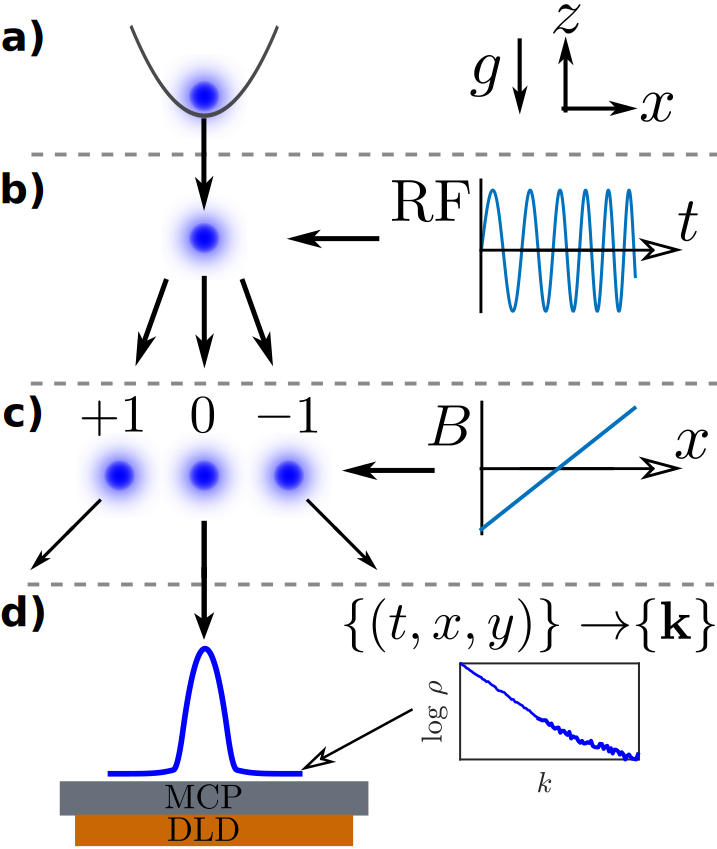
\includegraphics[width=0.4\textwidth]{fig/QD/main/main/exp_cartoon}
% %     \caption{Sketch of experimental sequence.
% 	A BEC is releaed from a harmonic trap (a) and expands during freefall before being split into a superposition of the $m_J\in\{-1,0,1\}$ states (b) by an rf chirp.
% 	A magnetic field gradient separates the clouds (c) ensuring that only the magnetically insentitive $m_J=0$ cloud lands on the detector (d), from which the momentum information is reconstructed.
% 	The quantum depletion lies in the dilute tails at large momentum (inset).}
% %     \label{fig:sequence}
% % \end{figure}

% % We interleaved the measurements just described with calibrations to determine the atom number, trapping frequencies, state transfer efficiency, and noise contributions (see supplementary materials for details).
% 	The trapping frequencies are stable to better than 1\% and the transfer efficiency was $\sim25\%$ in all runs, with an absolute variation of order $2\%$ within runs.
% 	We observed that a few remnant atoms from the $m_J=+1$ cloud were not completely removed from the detector.
% 	We minimized this effect by careful configuration of the magnetic field switching sequence, and calibrated for it by repeating the main measurement sequence without the rf transfer to the $m_J=0$ state.
% 	While readily measurable, the dark count rate was not significant.

% % % The k^4 thing naively induces an ultraviolet divergence, but this is avoided by considering microscopic details at momentum scales inacessible to this experiment

% % \section{Theory}
% % The two-body contact, the expectation value of the local density of pairs $\hat{C} = 32 \pi^2 a^2 \hat{n}^2$ \cite{Werner12_boson}, can be written in terms of the total energy $E$ through the \emph{adiabatic sweep theorem} \cite{Tan08_energetics},
% % \begin{equation}
% % \mathcal{C} = \frac{8\pi m a^2}{\hbar^2}\frac{\partial E}{\partial a}.
% % \end{equation}
% % The contact for a harmonically trapped gas in the Thomas-Fermi approximation is 
% % % which fixes the asymptotic momentum density as $\lim_{|\kvec|\rightarrow\infty}  n(\kvec) = \mathcal{C}/|\kvec|^4$ \cite{Tan08_momentum}, where $\kvec = m\vec{v}/\hbar$ is the single-particle wavenumber and $m$ is the atomic mass.
	
% % \begin{equation}
% % \mathcal{C} = \frac{8\pi}{7} \left(15^{2}(a N_0)^{7} \left(\frac{m \bar{\omega}}{\hbar}\right)^{6}\right)^{1/5},
% % \label{eqn:TotalHarmonicContact}
% % \end{equation}
% % which yields the asymptotic momentum density 
% % \begin{equation}
% % \lim_{|\kvec|\rightarrow\infty}  \rho(k) = \frac{64\pi^2a^2 }{7} \frac{n_0 N_0}{k^4},
% % \label{eqn:mom_dist}
% % \end{equation} where $n_0$ is the peak density of a condensate of $N_0$ atoms in a harmonic trap.
% 	Eqn.
% 	\ref{eqn:mom_dist} can be integrated to predicte the expected number of bosons with wavenumbers  $k\in (k_1, k_2)$.,
% % \begin{equation}
% % \mathcal{N}_{k_1,k_2} =\frac{\mathcal{C}}{\pi^2}\left(\frac{1}{k_1}-\frac{1}{k_2}\right),
% % \label{eqn:pred_num}
% % \end{equation}

% % The number $N_{k_1,k_2}$ of atoms detected in the region of interest thus directly yields an estimate of the contact via $C = \frac{\pi^2}{\chi\eta_0\Omega}\cdot \frac{k_1 k_2 N_{k_1,k_2}}{k_2-k_1}$, accounting for the detector efficiency $\chi$, the transfer rate $\eta_0$ into the $m_J=0$ pulse, and where $\Omega$ denotes the fraction of the spherical shell contained within our detector field of view and radially bounded by $k_1$ and $k_2$.
% 	 We chose $k_2=10\micron^{-1}$ to maximize the spherical collection volume while accounting for the limited field of view.
	


% % \section{Results} 
% % Fig.
% 	\ref{fig:cdfplot} (a) shows the number of detected atoms $N_{k_1,k_2}$, exhibiting the transition from the thermal to quantum-depleted region and asymptotic behaviour consistent with the prediction $\mathcal{N}_{k_1,k_2}$.
% 	Eqn.
% 	\ref{eqn:pred_num} provides a test for the presence of $k^{-4}$ scaling in the momentum density: Any other asymptotic scaling would manifest as a dependence of $C$ on $k_1$.
% 	Indeed, the empirical contact $C$ is not significantly dependent on $k_1$ in the region $k_1\in(6\micron^{-1},10\micron^{-1})$, as shown in \ref{fig:cdfplot} (b).
% 	Thus, despite detecting only a dozen atoms per shot on average, we find good evidence of the power-law decay in the region of interest.
% 	The uncertainty-weighted mean of the contact determined from the number of counts in the tail is 1.9(3) times the predictions from Eqns.
% 	\ref{eqn:pred_num} and \ref{eqn:TotalHarmonicContact} using parameters from the calibration measurements.
% 	The results of analysing our entire dataset are summarized in Table \ref{tab:results}.

% % \begin{figure}[t]
% %         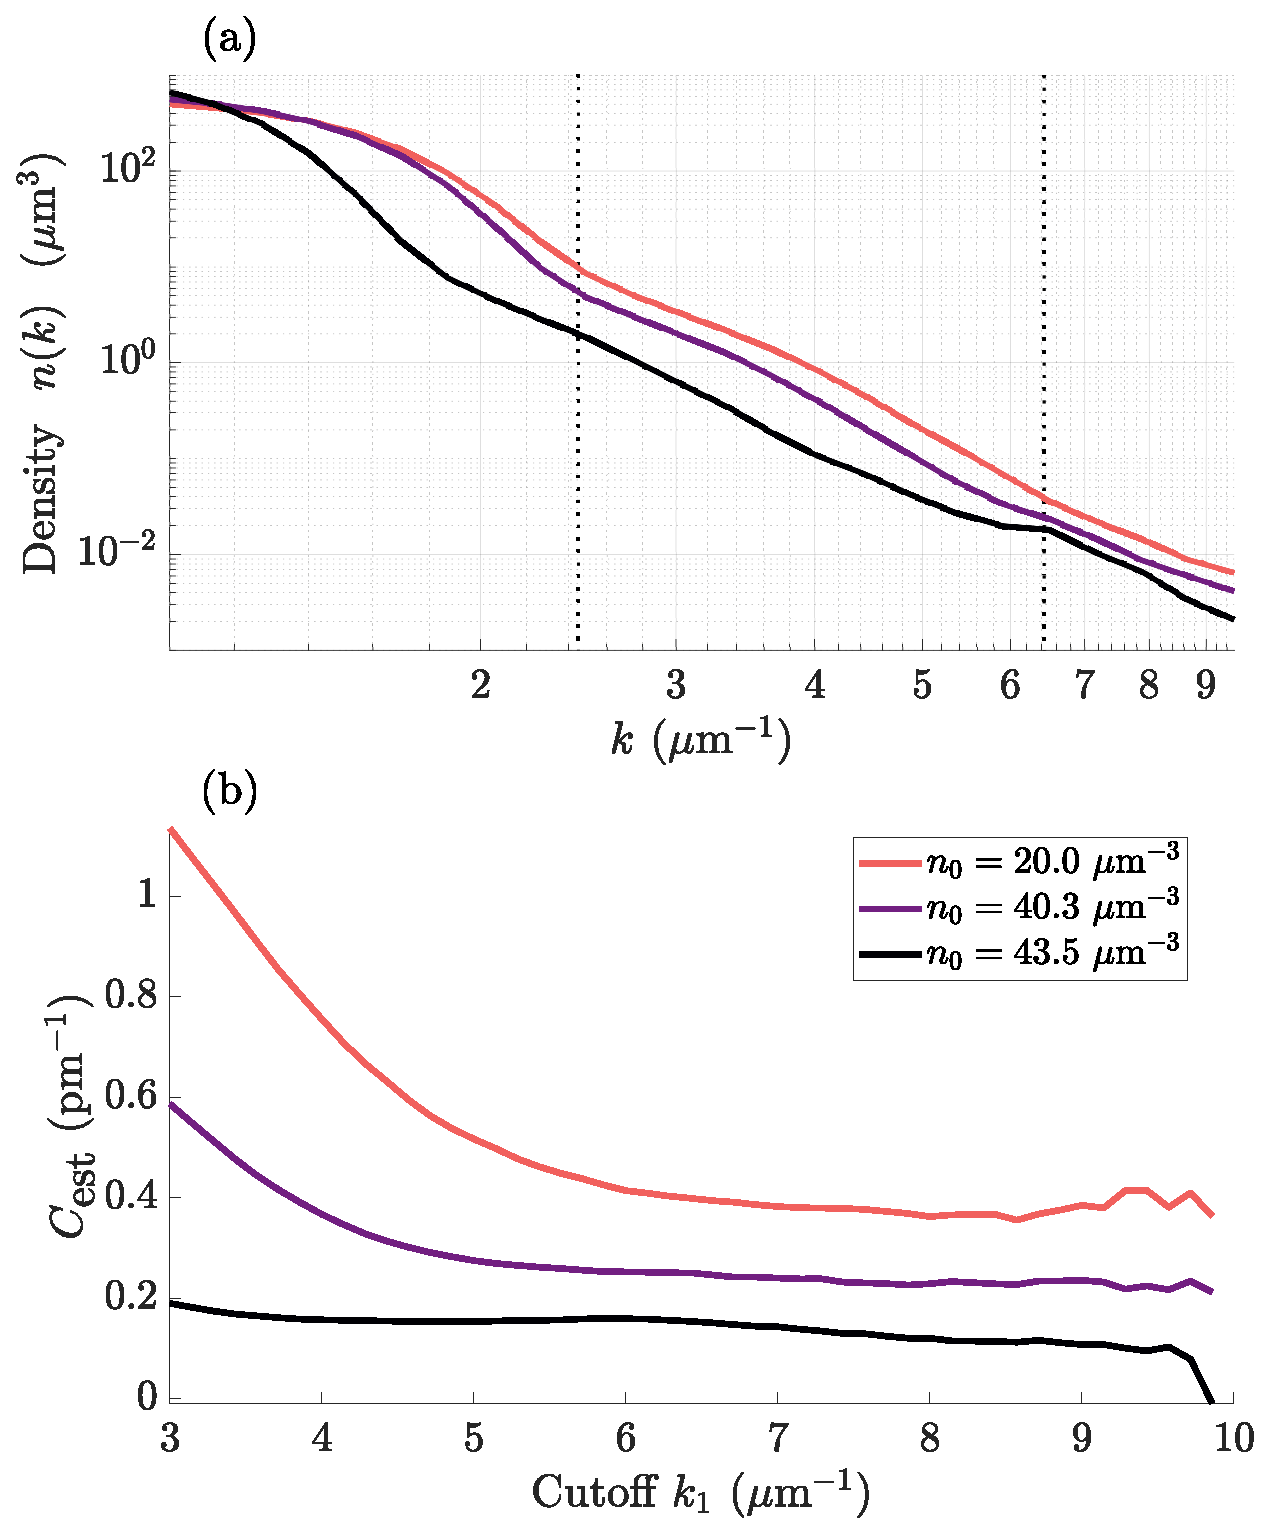
\includegraphics[width=0.5\textwidth]{fig/QD/main/main/contact_determination}
% %         \caption{Number of atoms detected in the region of interest.
% 	In (a), the mean of $N_{k_1,k_2}$ is shown for each run (solid lines), along with the predicted $\mathcal{N}_{k_1,k_2}$ (dotted lines), for fixed $k_2=10\micron^{-1}$.
% 	The tail amplitude computed via Eqn.
% 	\ref{eqn:pred_num} is shown in (b) as a function of the cutoff $k_1$, which behaves consistently with a $k^{-4}$-like scaling of the momentum distribution.}
% %         \label{fig:cdfplot}
% % \end{figure}







% % % Linear regression model:
% % %     y ~ 1 + x1

% % % Estimated Coefficients:
% % %                     Estimate        SE         tStat      pValue  
% % %                    __________    _________    _______    _________

% % %     (Intercept)         1.769      0.46851     3.7758    0.0054207
% % %     x1             2.3935e-08    3.927e-08    0.60949      0.55911


% % % Number of observations: 10, Error degrees of freedom: 8
% % % Root Mean Squared Error: 0.391
% % % R-squared: 0.0444,  Adjusted R-Squared: -0.0751
% % % F-statistic vs.
% 	constant model: 0.371, p-value = 0.559
    
% % \begin{figure}[b]
% %         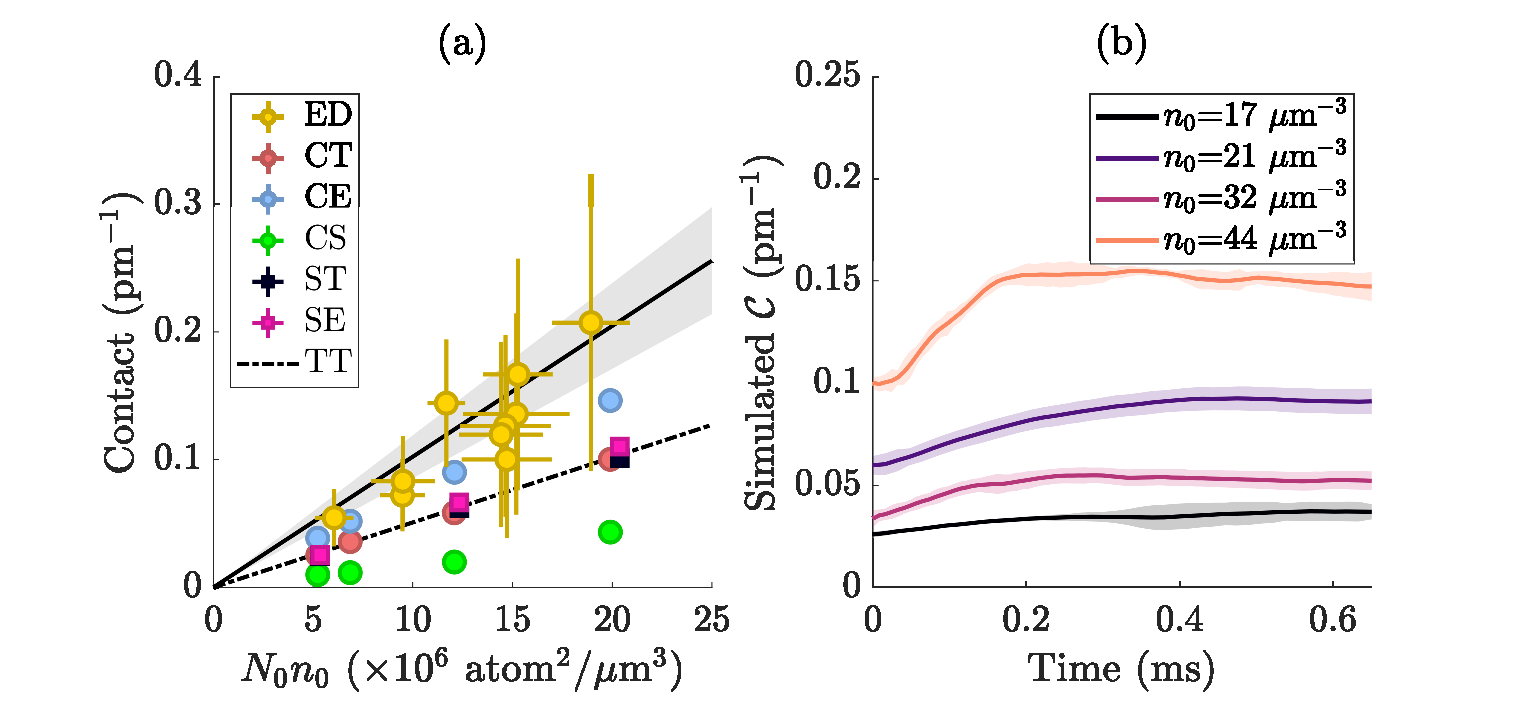
\includegraphics[width=0.5\textwidth]{fig/QD/main/main/contact_plot_with_theory}
% %         \caption{Comparison of simulations and experiments.
% 	(a) The contact from empirical data (ED) exceeds the prediction by the Tan theory (TT), with trend (and 1$\sigma$ confidence interval) shown as a solid line (grey area).
% 	The simulated contact of BECs in a cigar-shaped trap (CT) are consistent with (TT) before release but compare well with our measurements after expansion (CE).
% 	A slow relaxation of the tight axes of the cigar trap (CS) show a reduction in the large-momentum tails.
% 	Simulations of a spherical trap (ST) show a modest increase after expansion (SE).
% 	(b) Simulations of condensates released from a cigar-shaped trap show an increase in contact after the trap release, stabilizing after a time on the order of 100$\mu$s.}
% %         \label{fig:theory_fig}
% % \end{figure}

% % \begin{table*}[!t]
% %     \begin{tabular}{c c c c c c c}
% %     \hline\hline
% %     Peak density ($\micron^{-3}$) & $N_\textrm{tot}$ ($\times10^5$) & Thermal fraction & ROI counts & Expected counts & $C_\textrm{est}$ ($\times10^{11} m^{-1}$) &$C_\textrm{est}/\mathcal{C}$  \\ 
% %     \hline 
% %     16.9(1.8) & 3.5(4) & 0.09 & 5.6(0.1) & 2.8(0.6) & 5.4(2) & 1.9(0.8) \\ 
% %     18.7(1.4) & 5.0(4) & 0.17 & 6.8(0.1) & 3.7(0.8) & 7.2(3) & 1.8(0.7) \\ 
% %     19.3(2.1) & 4.9(6) & 0.08 & 8.1(0.2) & 4.3(0.9) & 8.3(4) & 1.8(0.8) \\ 
% %     20.4(1.0) & 5.7(3) & 0.09 & 14.8(0.1) & 5.5(1.2) & 1.4(5) & 2.6(0.9) \\ 
% %     38.6(2.6) & 3.9(3) & 0.14 & 4.9(0.1) & 1.9(0.4) & 1.6(9) & 2.5(1.3) \\ 
% %     38.6(3.4) & 3.7(4) & 0.09 & 3.5(0.04) & 1.9(0.4) & 1.1(7) & 1.7(1.0) \\ 
% %     38.6(3.5) & 3.8(4) & 0.11 & 3.7(0.1) & 2.4(0.5) & 1.0(6) & 1.5(0.9) \\ 
% %     38.7(3.4) & 3.7(4) & 0.09 & 4.1(0.1) & 2.1(0.4) & 1.2(7) & 1.8(1.0) \\ 
% %     39.0(4.1) & 3.8(5) & 0.10 & 4.3(0.1) & 2.2(0.4) & 1.3(8) & 1.9(1.1) \\ 
% %     41.3(2.2) & 4.5(4) & 0.12 & 6.5(0.2) & 2.6(0.5) & 2.0(1) & 2.4(1.3) \\ 
% %     \hline\hline
% %     \end{tabular}
% %     \caption{Summary of results for each data run.
% 	The peak density is determined from measurements of the condensed number (via the total number $N_\textrm{tot}$ and condensate fraction) and trapping frequencies, which in turn is used to predict the contact $\mathcal{C}$.
% 	The number of atoms detected in the region of interest can be used to determine the empricial contact $C$ from the $k^{-4}$-like tail by inverting Eqn.
% 	\ref{eqn:pred_num}}
% %     \label{tab:results}
% % \end{table*}

% % \section{Simulations} 
% % To gain further insight we performed simulations of the BEC expansion from a harmonic trap using the Positive-P method, including a cigar-shaped trap with parameters matched to the experimental conditions, and a spherically symmetric trap with identical peak density $n_0$.
% 	The results of these simulations are consistent with the adiabatic sweep theorem before release from the trap, and agree well with our experimental data, as shown in Fig.
% 	\ref{fig:theory_fig} (a).
% 	Following release from the trap, the simulated tail amplitude increased and stabilized at a factor of 1.46(5) above the predictions of \ref{eqn:TotalHarmonicContact} in a few hundred microseconds, much smaller than the 2ms delay between the trap release and application of the rf and Stern-Gerlach pulses.
% 	We also investigated the effect of adiabatic expansion on the in-trap contact by simulating a slow decrease of the trapping frequencies by a factor of two, and found that the in-trap contact decreased in these instances.
	


% % \section{Discussion} We interpret our results as an indication that dispersal of the mean-field energy of the condensate into kinetic energy of the depleted atoms is the mechanism responsible for the disagreement between predicted and measured contact.
% 	In detail, following the quench of the condensate into the free particle regime, the condensate expands hydrodynamically.
% 	This adiabatic reduction in density reduces the local contact density, whereby some depleted atoms are absorbed back into the condensate.
% 	However, the quasiparticles with large $k$ (in the particle branch of the Bogolubov dispersion) have sufficient velocity to escape the cloud before reabsorption.
% 	The relevant timescale for hydrodynamic expansion is on the order of millseconds, while the supersonic depleted particles leave the condensate in microseconds.
% 	Moreover, an atom inside the BEC experiences a force given by the gradient of the mean-field potential (and consequently the density) $F = 4\pi\hbar^2a \nabla  n(x)/m$.
% 	This increases the number of depleted particles with enough energy to escape reabsorption into the condensate, and endows the depleted particles with a greater velocity, leading to an increase in the weight of the tails in the far-field, and of particular relevance to lighter atoms because the acceleration scales with $1/m^2$.
% 	This picture is supported also by the simulations, in which we observe a decrease in the total number of depleted particles coincident with an increase in the large-k population.
	


% % \section{Conclusion}
% % In conclusion, our findings suggest that the quantum depletion is indeed visible in the far-field momentum distribution, and that the hydrodynamic approximation does not capture sufficient microscopic information to make detailed predictions about the high-momentum behaviour.
% 	The interplay between coherent absorption of Bogolubov excitations and the dispersal of the chemical potential into kinetic energy, to which Helium is particularly sensitive, result in overpopulation of the $k^{-4}$ tails of the momentum distribution.
	

% % \section{Future work}
% % The growing suite of far-field investigations \cite{Cayla20,Chang16} supplemented by this work invite complementary studies of the quantum depletion and contact in situ with ultracold \mhe.
% 	Measurements of the structure factor via Bragg spectroscopy may greatly benefit from the single-particle detection afforded by metastable Helium, which is compelling in light of complications of radio spectroscopy of Helium (discussed in the supplementary material).
% 	An intriguing goal for future studies in Helium is the resolution of particle pairs with opposite momenta in the depleted fraction.
% 	 Such an observation would be challenging because the correlation peak height decreases with the collection efficiency and is broadened by the expnsion dynamics.
% 	Nonetheless, insight into pairing mechanisms in a cold bosonic gas would bear fruit for wider coherent phenomena in condensed matter.


% %     % Leo 2001: The M pairings (1,1),(1,0),(-1,-1), and (-1,0) the collision is dominated by a $^5\Sigma_g ^+$ potential, hence \emph{inelastic processes can occur only via the weak relativistic spin-dipole interaction}.
% 	The scatteering lengths are then almost identical to $a_5$ but with small imag part.
% 	Ilastic rates for (0,0) and (1,-1) from which ionization can occur, are much larger and dominate the total ionization rate for an unpolarized gas.
	
% %     % Ergo - could use RF spectroscopy by modulating the ion production rate via the (1,-1) channel?
% %     % Vassen: $a_{1,-1} \approx 60a_0, a_{1,1} \approx 140 a_0$.
% 	But the chemical potential for each species is different - does this shift the RF resonance? Or affect the ion production rate?
% %     % -> Ion production rate in terms of scattering lengths, spin pol etc?
% %     % -> Find ion production rate from majorana flips: Majorana flip rate x 
% %     % I wonder if contact measurements could just be extracted from the data that Vassen took in 2016?



% % \section{Appendices}
% % \section{Detection}
% %     We use a Roentdek DLD80 multichannel plate and delay-line detector stack \cite{Manning10} with a quantum efficiency of $\sim8\%$, and space and time resolutions of 100 $\mu$m and 3 $\mu$s, respectivel
% 	After the atoms are released from the trap, they fall 859mm to the detector stack, which registers the arrival times and positions $(t_i,x_i,y_i)$ of each atom, indexed by $i$.
% 	The centre of mass of the cloud arrives after a $\tau = 417$ms time of flight.
% 	The velocity of each atom relative to the centre of mass of the cloud is $(v_x,v_y,v_z) = t_{i}^{-1}(x_i,y_i,g_0(\tau^2-t_{i}^{2}))$, where $g_0$ is the local gravitational acceleration.
% 	The velocity conversion carries a negligible error of a few ppm.
% 	We then centre the counts from each realization and detection sequence (termed a \emph{shot}) and transform the counts from cartesian velocity space to spherical polar coordinates with radius $k$ (in $m^{-1}$), polar angle $\theta$ and elevation angle $\phi$, relative to the centre of the cloud, where the velocity-to-wavevector transformation follows from  $\textbf{p}=m\textbf{v}=\hbar\textbf{k}$.
	

% %     The solid angle in k-space available to detect the depleted tails is limited by the 40mm radius of the circular detection surface.
% 	The field of view of our detector is $|k_{x,y}|\approx5\times 10^6$ m$^{-1}$ in the XY plane, which is only just sufficient to reach past the edge of the thermal region.
% 	We sample data from the segments of the sphere with elevation angle $|\phi|>\pi/3$ rad and $|k|<10^7$ m$^{-1}$, centred on the BEC, which encompasses a total solid angle of $0.22\times 4\pi$ steradians.
% 	The detector's dark count rate of $0.56$ Hz cm$^{-2}$ sets the noise floor and contributes an average of 0.4(2) counts to the region of interest per shot.
% 	The distribution of the number of counts in each shot are shown in Fig.
% 	\ref{fig:num_counts}


% % \begin{figure}[!h]
% %     \centering
% %     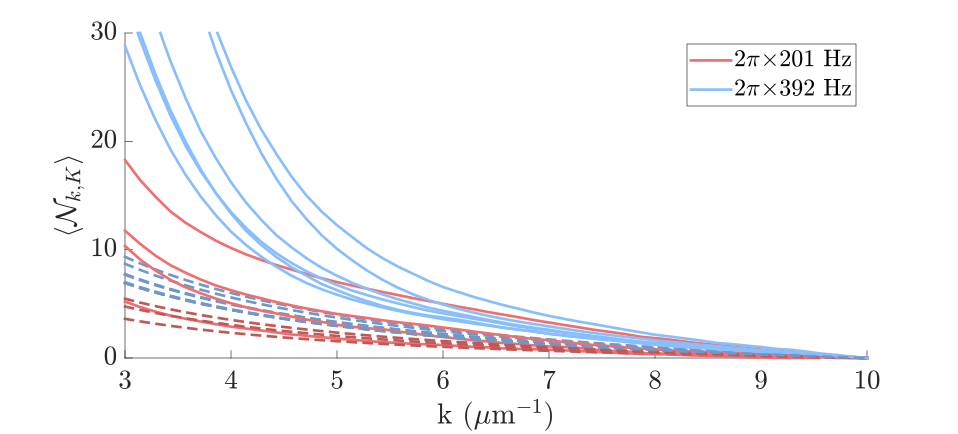
\includegraphics[width=0.7\textwidth]{fig/QD/main/som/counts_per_run}
% %     \caption{Number of counts detected in the region of interest across in the depletion measurement (a), the spin mixing calibration (b), and the dark count calibration (c).
% 	An average of 3.0(5) counts were detected in the ROI in the spin-mixing calibration shot, and the background count rate was 0.4(2) counts per shot.}
% %     \label{fig:num_counts}
% % \end{figure}

% % % \todo{Density plots out to larger $|k|$ to show descent into noise floor? How far could we push it until we hit dark counts?}

% % % \section{Spin mixing}
% % % Also lets us determine thermal fraction - note it isn't determinable from the PAL because of the mean-field broadening (but one could just make fits and subtract the thermal part, yes?).
% 	I think the mean-field expansion is particularly bad for Helium, and wasn't reported much before, because we are 5% the mass of popular species like Rb so much more subject to mean-field acceleration!

% % \section{Trap configuration and calibration}

% %     We prepared our BECs with a standard sequence, achieving condensation via forced evaporative cooling in a harmonic magnetic trap with trap frequencies $\sim(425,425,45)$ Hz and a DC bias stabilized by our auxiliary field compensation coils \cite{Dedman07}.
% 	For the tight trap we increased the coil current after the cooling sequence to obtain trapping frequencies $\sim(902,895,71)$ Hz, using a sigmoid step function which to minimize in-trap oscillations.
% 	The trap remained on for 150ms before switching the trap off with a $1/e$ time of $\approx38\mu$s.
% 	The condensates were allowed to expand for 2ms before we transferred some of the condensate into the magnetically insensitive $m_J=0$ state to prevent distortion by stray magnetic fields.
% 	The rf RF sweep generated by a RIGOL function generator, amplified, and applied to the experiment chamber by a coiled antenna inserted into the BiQUIC coil housing.
% 	The pulse swept from 1.6-2.6MHz over 1ms and was centred on the fine structure resonance between the $m_J$ states and transfers atoms into the $m_J = j$ states with efficiencies $\eta_j$.
% 	The sweep was $10^6$-fold wider than the Doppler broadening of the BEC which ensures uniform transfer at all momenta.
% 	Immediately after the RF sweep, the bias coils are switched off and auxiliary push coils in the vertical (Z) and weak horizontal (X) axis are activated using a fast MOSFET switch to implement a Stern-Gerlach separation of the $m_J = -1,~0,$ and $+1$ pulses

% % \subsection{Determining transfer efficiency}

% %     To calibrate the transfer efficiencies, we applied the Stern-Gerlach field for a shorter time, resolving each cloud on the detector.
% 	While the efficiencies $\eta_J$ cannot be calculated by counting the atoms in each cloud because the detector saturates, we can compare the thermal parts.
% 	We align each cloud along the time axis and compute the pointwise proportion of the atomic flux accounted for by each cloud, as depicted in Fig.
% 	\ref{fig:frac_cal}.
% 	The flux fraction of each cloud is roughly constant in the thermal part, indicating the absence of important saturation effects and a spin transfer that is independent of $k$.
% 	The fraction of the total flux of each pulse is identified with the fraction of the original cloud which has been transferred into the respective spin state.
% 	We find these efficiencies are approximately 74\%, 24\%, and 2\% in all runs for the $m_J=+1$, 0, and -1, respectively.
	 
    
% % \begin{figure}[!h]
% %     \begin{center}
% %         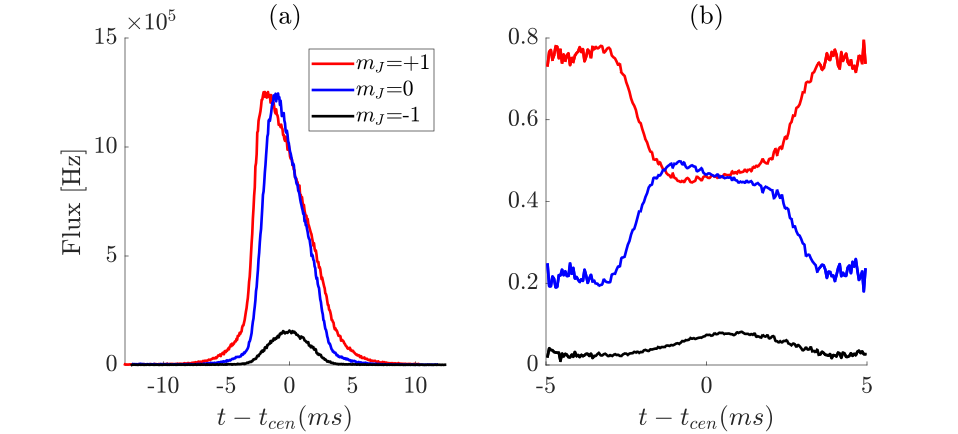
\includegraphics[width=0.7\textwidth]{fig/QD/main/som/frac_cal_profile}
% %         \caption{Determining the rf transfer efficiency.
% 	The time-of-flight profiles of each pulse are aligned with respect their centre-of-mass (a).
% 	The pointwise fraction ((b), dotted line) is uniform where saturation is not evident (solid lines).
% 	Detector saturation is apparent in the peaks of the $m_J=+1$ and $m_J=0$ pulses, but not in the $m_J=-1$ pulse.}
% %         \label{fig:frac_cal}
% %     \end{center}
% %     \end{figure}


% % \subsection{Determination of thermal fraction}
% %     While the $m_J=0$ and $m_J=1$ clouds clearly saturate the detector, the small fraction ($\sim2\%$) in the atoms to the $m_J=-1$ state  does not.
% 	We fit the density outside the condensate with a Gaussian distribution plus constant background and obtain an estimate of the thermal atom number.
% 	Subtracting the number of thermal atoms from the total number in the $m_J=-1$ cloud, minus background counts, yields a estimate of the thermal and condensed fraction, as illustrated in Fig.
% 	\ref{fig:thermal_frac}.

% %     \begin{figure}[!h]
% %     \begin{center}
% %         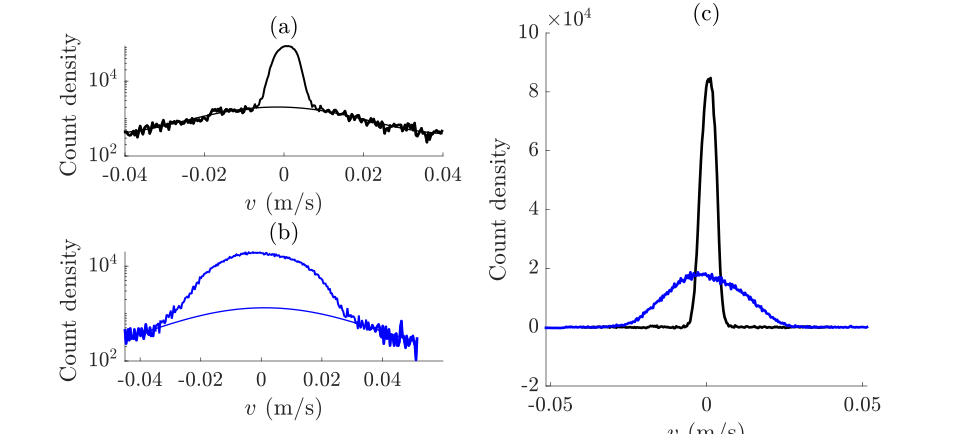
\includegraphics[width=0.7\textwidth]{fig/QD/main/som/m1_frac_anal}
% %         \caption{Comparison of thermal fits in the unsaturated $m_J=-1$ pulse including 138 shots.
% 	The weak (X) and strong horizontal (Y) trapping axes are shown in (a) and (b), respectively.
% 	Both projections display a bimodal peak, with the condensate (dotted lines) and thermal parts (thick solid lines) easily distinguished.
% 	Fitting a Gaussian profile (thin solid line) to the velocity distribution of the thermal part yields the thermal number and temperature.
% 	Subtracting the fit leaves the condensate profile (c) which can be yields the condensed number.}
% %         \label{fig:thermal_frac}
% %     \end{center}
% %     \end{figure}



% % \subsection{Analysis of spin transfer measurements}

% %     In early tests of our measurement sequence we noticed a contamination of the signal by spurious counts from the $m_J=+1$ cloud.
% 	We calibrate for this contamination by running the depletion measurement without the RF transfer.
% 	While the cause of the cross-contamination is unclear, we observe that the count density outside the region of interest is similar in both the shots with the RF pulse and those without.
% 	We infer that the remnant counts may be atoms transferred into the $m_J=0$ state by a side effect of the finite switching time of the magnetic fields.
	

% %     % \begin{figure}[!h]
% %     % \begin{center}
% %     %   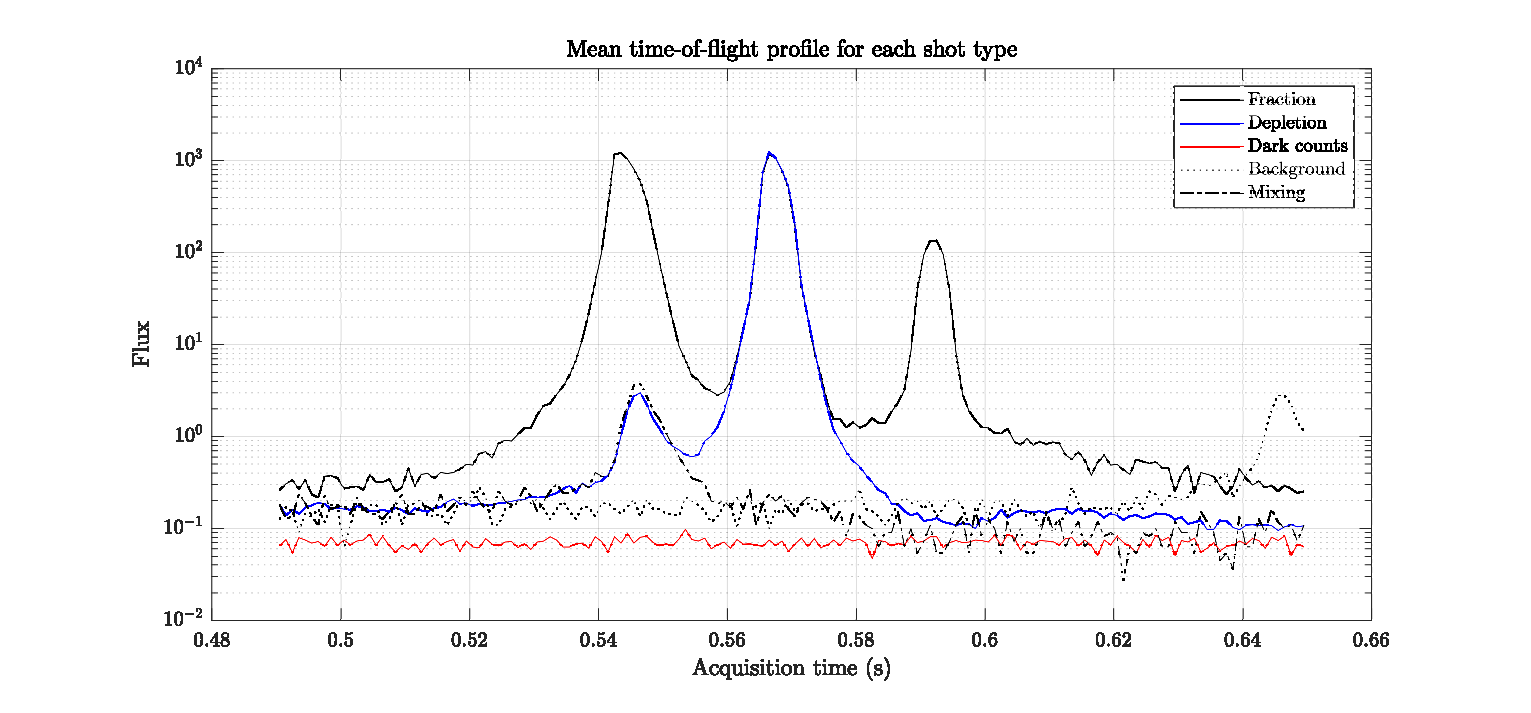
\includegraphics[width=\textwidth]{fig/QD/main/som/profile_overlay}
% %     %   \caption{Comparison of average time-of-flight profiles over a single data run for the quantum depletion measurement shots (blue, 871 shots), transfer efficiency calibration (black, 112 shots), detector dark counts (red, 871 shots), and spurious counts (dot-dash, 895 shots).
% 	The time window bounded by $|k|\leq 10\mu$m is indicated with dotted lines.
% 	Shaded area is the standard error over the entire run.}
% %     %   \label{fig:tof_profile}
% %     % \end{center}
% %     % \end{figure}




% % % Note that the temps disagree between axes, but within axes between clouds they are consistent(....ish).
% 	This means we can use the profile ratio method, which is also consistent with comparing the thermal number from the fits.
% % % Perhaps comment on the thermal-subtracted part; the TF profile should have a sharp cutoff, but the smooth edges are suggestive evidence of this roll-off


% % \subsection{Peak density calibration}

% %     The peak density of the condensate can be written as $n_0 = \mu/g$, where $\mu$ is the mean-field energy in the Thomas-Fermi approximation and $g=4\pi\hbar^2a_{1,1}/m$ is the effective interaction strength, in terms of the atomic mass $m$ and $a=7.512$ nm is the s-wave scattering length between pairs of atoms in the $m_J=1$ state \cite{Moal06}.
% 	The expression for the peak density can can be expanded as
% %     \begin{equation}
% %         n_0 = \frac{1}{8 \pi}\left( (15N_0)^2 \left(\frac{m \bar{\omega}}{\sqrt{a_{1,1}} \hbar}\right)   ^{6}\right)^{1/5}
% %         \label{eqn:n0}
% %     \end{equation}
% %     where $\bar{\omega} = \left(\omega_x\cdot\omega_y\cdot\omega_z\right)^{1/3}$ is the geometric trap frequency and $N_0$ is the number of atoms in the condensate.
% 	We simultaneously determine the total atom number $N$ and trap frequency $\bar{\omega}$ in a single shot using a pulsed atom laser and use the thermal fraction to determine the condensed number $N_0$.
	

% %     The pulsed atom laser consists of a series of Fourier-broadened RF pulses centred on the minimum Zeeman splitting in the trap.
% 	The pulse transfers atoms in the trap to the untrapped $m_J=0$ state with an approximately constant transfer rate across the cloud.
% 	We outcouple approximately 2\% of the atoms per 100$\mu$s pulse for $\sim$200 pulses, which eventually depletes the entire trap.
% 	The atom laser thus prevents the detector from saturating and allows an accurate determination of the atom number, up to a factor of the quantum efficiency.
% 	A typical outcome of this procedure is shown in Fig.
% 	\ref{fig:pal_shot}

% %     \begin{figure}[!h]
% %     \centering
% %         \includegraphics[width=0.7\textwidth]{fig/QD/main/som/pal_shot}
% %         \caption{A kicked pulsed atom laser with motion sampled at 11ms intervals.
% 	The oscillations in the centre-of-mass position of each pulse are shown along the Y axis over time (a).
% 	The apparent frequency can be determined for each axis (b).
% 	The outcoupling efficiency is fixed throughout the sampling sequence (c), producing a geometric decay of the number of atoms in each pulse.
% 	The straight line on a logarithmic scale shows that detector saturation saturation is negligible and that the BEC population does not affect the transfer rate.}
% %         \label{fig:pal_shot}
% %     \end{figure}
    
% % \subsection{Measuring the trapping frequencies}

% %     To illustrate how we obtain the trapping frequencies, consider an undamped harmonic oscillator in one dimension.
% 	The centre-of-mass momentum $p(t) = A \cos(2\pi f t))$ oscillates at a frequency $f$ Hz, and the centre of mass of a pulse outcoupled at time $t'$ lands on the detector at a position $x'(t+\tau) = p(t')\tau/m$, where $\tau$ is the time of flight of the centre of mass.
% 	Sampling the cloud motion with a sampling period T starting at initial time $t_0$ produces a series of pulses whose centres of mass land at $\{x_n = (A\tau/m) \cos(\omega(t_0+nT))\}$.
% 	The sampling frequency $f_s=1/T$ determines the \emph{Nyquist frequency} $f_N=f_s/2$, which is the maximum frequency that can be reconstructed unambiguously from such a sampling regime.
% 	When $f>f_N$ the signal manifests as a lower-frequency oscillation known as the \emph{alias} of the signal.
% 	The aliased frequency $f_a$ is

% %     \begin{equation}
% %      f_a =
% %       \begin{cases}
% %        \frac{Z_n f_s}{2} - f & \text{if } Z_n \text{ even} \\
% %        f - \frac{(Z_n-1)f_s}{2}       & \text{if } Z_n \text{ odd},
% %       \end{cases}
% %       \label{eqn:Z_N}
% %     \end{equation}
    
% %     where $Z_n = \lceil{f/f_N}\rceil$ is the Nyquist zone number, as described in numerous rf engineering references.
% 	While it is not possible to determine $Z_N$ for a signal with an unknown (not necessarily stationary) $f$ from samples taken at a fixed $f_s$, one can vary $f_s$ and determine both $Z_N$ and $f$ from the gradient $d f_a / d f_s$.
	
% % \begin{figure}[!h]
% %     \centering
% %         \includegraphics[width=0.7\textwidth]{fig/QD/main/som/sawtooth_plot}
% %         \caption{Aliasing of the trap frequency oscillations under different sampling regimes.
% 	The fitted oscillation frequency is shown in each axis for a range of sampling frequencies.
% 	The sawtooth function is a one-parameter fit which determines the underlying frequency of the centre-of-mass oscillations.}
% %         \label{fig:sawtooth_plot}
% %     \end{figure}    

% %     We induce oscillations of the BEC in all three axes by briefly displacing the trap centre with a perturbation to the trapping field.
% 	The maximum sampling frequency is limited by the temporal width of the BEC pulse landing on the detector to about 100Hz, yielding a Nyquist frequency too low to resolve the un-aliased oscillations.
% 	We fit the apparent oscillation frequency in each axis as a function of sampling frequency as shown in Fig.
% 	\ref{fig:sawtooth_plot}, along with a one-parameter fit of Eqn.
% 	\ref{eqn:Z_N}.
% 	We thys determine that the frequencies $(\omega_x,\omega_y,\omega_z)$ of each of the traps used in the experiment are $2\pi\times(45,425,425)$ and $2\pi\times(72,889,893)$, respectively, which are stable to within 5\% throughout the duration of the data collection and to better than $1\%$ in a given run.


% %     \section{Theory}

% % In the Thomas-Fermi approximation, the energy per particle of $N_0$ condensed bosonic atoms is
% % \begin{equation}
% % \frac{E}{N_0} = \frac{5}{7} \mu = \frac{5}{7} \frac{\hbar \bar{\omega}}{2} \left(\frac{15 N_0 a}{a_\textrm{HO}}\right)^{2/5},
% % \end{equation}
% % in terms of the chemical potential $\mu$, where $a_\textrm{HO} = \sqrt{\hbar/(m \bar{\omega})}$ is the harmonic oscillator length \cite{PethickSmith}.
% 	Via the sweep theorem it follows that
% % \begin{equation}
% % \mathcal{C} = \frac{8\pi}{7} \left(15^{2}(a N_0)^{7} \left(\frac{m \bar{\omega}}{\hbar}\right)^{6}\right)^{1/5}.
% % \label{eqn:TotalHarmonicContact}
% % \end{equation}

% % Which by substitution of Eqn \ref{eqn:n0} leads to the expression
% % \begin{equation}
% % \mathcal{C} = \frac{64\pi^2a_{1,1}^{2}}{7}\frac{n_0N_0}{k^4}.
	
% % \label{eqn:TotalHarmonicContact}
% % \end{equation}

% % The Lee-Huang-Yang (LHY) correction to the condensate energy is negligible in our experiments.
% 	The LHY correction for the chemical potential of a uniform condensate with density yields an estimate of the worst-case contribution
% % $$
% % \frac{\partial E}{\partial a_{1,1}} = \mathcal{C}_0\left(1+\frac{64\sqrt{na_{1,1}^{3}}}{3\sqrt{\pi}}\right),
% % $$
% % Where $\mathcal{C}_0$ is the contact computed neglecting the LHY term, and the second term in brackets is the LHY correction which amounts to at most a correction of order 1\%, using the highest $n_0$ observed in our experiments.
% 	In reality the correction will be smaller as the density is not uniform and is bounded above by $n_0$.

% % \subsection{Radio spectroscopic prospects}
% % The basic principle of rf contact spectroscopy is to apply an rf tone which is detuned from the resonance between two spin states, whereby atoms in the initial spin state are coupled to an untrapped channel, thus enabling a differential measurement of the atom number.
% 	The signal strength scales with the difference of reciprocal scattering lengths $\Gamma\propto(1/a_\textrm{i,i}-1/a_\textrm{i,f})$ between initial-initial and initial-final spin states \cite{Braaten10,Wild12}, which can be manipulated via Feshbach resonance to obtain a good signal.
% 	For He$*$ (spin 1) however, the scattering lengths $a_{1,1}$ and $a_{1,0}$ are identical \cite{Leo01}, rendering the preferred $m_J=1-m_J=0$ transition unusuable.
% 	On the other hand, $a_{1,-1} = 3/7 a_{1,1}$ \cite{Vassen16}, and the singlet transition can be driven without populating the $m_J=0$ state.
% 	In principle this could produce a detectable flux of atoms to perform sensitive in-trap contact measurements, however, collisions in the $^1\Sigma_{g}^{+}$ channel have large Penning ionization rates which lead to significant trap losses \cite{Leo01}.
% 	 The ionization products would be detectable by in-vacuum channel electron multipliers but require theoretical work to disentangle from the spectroscopic signal.
% 	Further, such an experiment could not take advantage of a Feschach resonance to increase signal strength or decrease the ionization rate, but it is not \emph{prima facie} impossible.

% % \section{Theoretical methods}
% % To fill in with details of how the P+ simulations were done by Piotr

% % \section{Old material}


% % \subsection{Detection of ultradilute momentum spectra}
% % \label{ssec:qd-model}

% %     Our experiments start with a condensate of helium atoms in the $m_J = +1$ state of the metastable $2^3 S_1$ manifold in a BiQUIC magnetic trap \cite{Dall2007}.
% 	The strongest signal of the depleted tails could be obtained by releasing the BEC from the trap and examining the tails of the detected flux on the detector.
% 	However, the presence of stray DC and transient fields in the chamber would distort the BEC profile and thus also the depletion, in ways that may not be feasible to characterize.
% 	For instance, it is known that our freefall zone contains what is colloquially known as a 'magnetic aperture', which deflects atoms from their freefall trajectory if their transverse momentum is great enough.
% 	This effect is visible in NONEXISTANT FIGURE, which shows the distortion of a thermal cloud, which would otherwise be isotropic.
% 	Indeed, this feature proved problematic in determining the detected count rate from the depleted fraction, because .
% 	Following the method described by Chang \emph{et al} \cite{Chang16}, substantial distortions to the condensate can be avoided by transferring part of the sample to the $m_J=0$ state, which is insensitive to stray magnetic fields.
	

% %     Since for these experiments a precise knowledge of the total atom number and trap frequency is important, we measure the trapped population and trapping frequency at regular intervals throughout each experimental run, using a procedure that avoids detector saturation to measure the atom number and precise determination of the trap frequency.
% 	We identified a contamination of the depletion signal by stray counts attributable to the $m=+1$ state, and calibrate for this by including shots without the RF transfer step.
% 	We also apply corrections for the detector dark count rate and an increased background rate on the leading edge of the condensate, which is attributed to a steady-state leakage of atoms from the trap, due to Majorana flips, Penning ionization, or other collisional effects driving loss.
	

% %     A magnetic field gradient is switched on 5ms after the state transfer pulse, which ensures the magnetically sensitive $M_J = \pm 1$ states are deflected enough to miss the detector.

% %     Since for these experiments a precise knowledge of the total atom number and trap frequency is important, we developed an experimental procedure to regularly calibrate the trapped population and trapping frequency at regular intervals throughout each experimental run, using a procedure that avoids detector saturation to measure the atom number (see supplementary material).
% 	We varied total atom number between 1 and $5\times 10^5$ atoms per condensate by varying the endpoint of the evaporative cooling ramp.

% %     We use two trap configurations with characteristic frequencies $\sim 2\pi\cdot (312,312,52)$ and $2\pi\cdot 666,666,69)$ Hz, which were calibrated on setup by the pulsed atom laser method described earlier in chapter XXX.
	

% %     As in previous chapters, data acquisition shots are interleaved with calibration measurements to predict the key variables 

% %     The trap is switched off in $\sim 100\mu s$ and the atoms allowed to fall 848mm, where they are detected with a multi-channel plate and delay line detector \cite{Manning2010}.
% 	To avoid distortion of the condensate by stray magnetic fields, we transferred approximately 25 - of the condensate into the magnetically insensitive $M_J=0$ state by applying a chirped sine wave 2ms after trap switch-off, swept from 1.6 to 2.6 MHz in 1ms, while a DC magnetic field remained on to preserve the Zeeman splitting between $M_J = {0,\pm 1}$ states.
% 	A magnetic field gradient is switched on after the state transfer pulse, which ensures the magnetically sensitive $M_J = \pm 1$ states are deflected enough to miss the detector.
	

% %     After release from the trap the atoms expand ballistically into the far-field regime, where their position on the detector corresponds to their momentum at trap release.
% 	Therefore we can reconstruct the far-field momentum distribution $n^*(\textbf{k})$ from our detector data.
% 	The observed momentum profile $n^*(\textbf{k})$ cannot be identified completely with the in-trap momentum distribution $n_0(\textbf{k})$ as repulsive interatomic forces distort the profile immediately after release from the trap.
% 	Structure is visible over five orders of magnitude in density, comprised of the condensed, thermal, and depleted fraction before the signal drops below the dark-count background noise.
% 	There is some saturation evident around the low momentum values due to the high atom flux during BEC impact.
% 	Our analysis does not include this part of the momentum profile, and we find evidence that saturation is only an issue during the peak flux, not in the thermal or depleted fractions.

% % The count density from the falling BECs depend explicitly on the trapped population and on the trapping frequencies, necessitating regular calibration of the peak condensate density.
% 	The correction from the detected $m_J=0$ counts to the full condensate profile also requires a measurement of the transfer efficiency of the RF pulse, and a diagnostic of any other sources of detection events, such as detector dark count rate or remnant atoms from the $mJ=\pm 1$ condensates.
% 	In the remainder of this section, I describe the means by which the relevant parameters are calibrated and how they are combined into a model of the detector flux which includes the Tan contact as a free parameter.
% 	In the next section, I describe the algorithm I designed to transform the atomic detection events into an appropriate format to correspond with the model and determine the Tan contact.

% % \subsubsection{Contributions to the model}
    
    
% % \subsubsection{Depletion}
% %     In an ideal world, the experimental procedure is trivial: Form a BEC in a desired trapping configuration, and then release the trap instantaneously and fit the atomic density profile obtained from the DLD image.
% 	Unfortunately, nature intervenes: Because our condensates are formed in a weak-field-seeking state, they are subject to deflection during freefall by stray DC and transient magnetic fields.
% 	These distortions to the BEC profile may be significant at large momenta, although we did not characterize this.
% 	A second potential issue is detector saturation, whereby the trailing side of the BEC is detected with a lower quantum efficiency because of a depletion of charge carriers in the MCP, artificially attenuating the depletion signal.
% 	Both of these issues are ameliorated by transferring a fraction of the condensate into the magnetically insensitive $m_J=0$ shortly after the trap release.
% 	This is achieved by sweeping an RF pulse from 1.6MHz to 2.6MHz, as in \cite{Chang16}, with a DC bias field held on by the Nuller coils.
% 	This field is close to uniform over the scale of the BEC and its freefall path, so by the time the condensate is split into the three spin states, distortions to the cloud would be minimal.

% %     The detection sequence therefore proceeeds with a standard BEC production sequence (as described in INTRODUCTION), with a modified end sequence, pictures in figure QD-SEQUENCE.
% 	The DC bias field is ramped on over 300ms in an exponential ramp with time constant 40ms.
% 	This ensures that no centre-of-mass oscillations are induced in the BEC because of sudden displacements of the trap centre.
% 	The BEC is held for XXX ms to damp out any residual oscillations and is then released.
% 	After 2ms of freefall, the RF chirp is generated by a RIGOL function generator, amplified, and applied to the experiment chamber by a coiled antenna inserted into the BiQUIC coil housing.
% 	The nuller coils are switched off, and the auxiliary push coils in the vertical (Z) and weak horizontal (X?) axis are activated via fast MOSFET switch.
% 	The pulse timing and duration of the push coils required some finessing to minimize the scatter of atoms from a \emph{magnetic aperture} inside the freefall path, as described in later in this section.
% 	The push coils remove the $m_J=\pm 1$ atoms from the detector, so the detector signal is dominated by the undistorted $m_J=0$ cloud.
% 	The cloud then falls freely under gravity through the vacuum chamber, completing the 848mm fall in 417ms.
	

% %     It is important to align the condensates carefully in order to faithfully extract the large-momentum tails.
% 	With an ideal detector, one could simply take the mean of all detected counts.
% 	Because of detector saturation, however, the mean position is heavily biased toward the leading edge of the BEC, and indeed the median (which is robust to outliers) is biased also (it is less robust to skewness).
% 	A workaround can be found in the threefold reflection symmetry of the condensate: The parabolic profile in each principal axis means that if one can identify the edges of the condensate, the centre of mass is at the midpoint along each axis.
% 	This is the basis of the following centering algorithm: For each axis, the atomic detection events are compiled into a histogram as a discrete approximation to the continuous atomic flux.
% 	The region where atomic flux exceeds the background rate by a factor of X is determined to be the BEC region - the extremal positions (or times) with flux above the threshold determine the edges of the condensate, and the mean of these two values determines the centre.
% 	The stages of this algorithm are depicted in figure CENTERING, along with the variation of the BEC centre over the course of a run.
	 

% %     We are concerned with the momentum-space distribution of counts.
% 	The atomic wavevector is related to the in-trap velocity by $\textbf{p}=\hbar\textbf{k} = m\textbf{v}$.
% 	The tranformation from $\textbf{r}-\textbf{r}_0$, where $\textbf{r}_0$ is the centre-of-mass position, is simply a linear transformation $\textbf{v} = \frac{\textbf{r}-\textbf{r}_0}{t_{tof}}$ in the $x$ and $y$ directions.
% 	For $z$, corrections must be made for gravitational acceleration instead given by solving the ballistic trajectories $v_z=-h/t_{tof}-\frac{1}{2}g*t_{tof}$ where $h$ is the fall distance and $g$ is the acceleration under gravity.
% 	\todo{txy-to-vel vs linear error?}

% %     The centred velocity-space counts are then transformed into spherical polar coordinates.
% 	The algorithm is described here is also used for the spin-mixing and dark count calibrations, where the spherical coordinate system is centred at the mean BEC centre-of-mass position in TXY coordinates.
	
% %     \begin{equation}
% %     	(r_i,\theta_i,\phi_i) = (\sqrt{x_{i}^{2}+y_{i}^{2}+z_{i}^{2}},\tan^{-1}(y_i/x_i),\tan^{-1}(z_i/\sqrt{x_{i}^{2}+y_{i}^{2}})
% %     \end{equation}

% %     The counts for each BEC are then compiled into a spherical histogram
% %     \begin{equation}
% %     	N(R(n),\Theta(l),\Phi(m)) = |\{(r_i,\theta_i,\phi_i:r(n)\geq r_i<r(n+1),\theta(l)\geq \theta_i<\theta(l+1),\phi(m)\geq \phi_i<\phi(m+1)\}
% %     \end{equation}
% %     Where $n,l,m$ are indices of the histogram with edges $r(n)$.
% 	Ergh, get this notation sorted out.
	
% %     The memory demands can get exhaustive - holding large TXY datasets and also lots of large 3D histograms - can reduce the by lots of writing to disk, but the cheater way around this was to compute the mean by adding to the histogram by looping over each shot, and ditto the squared number of counts to find the variance later.
% 	There would also be a biasing effect by including the empty bins which are defined outside the detector area.
% 	These are found by a messy case analysis in \verb|find_final_bin_idx.m| (hyperlink to dox html?).
% 	 These are excluded from subsequent sums over profiles.
% 	The bins are normalized by the spherical volume element
% %     % \begin{equation}
% %     \begin{align}
% %     	V(n,l,m) &= \int_{R(n)}^{R(n+1)} d r \int_{\Theta(l)}^{\Theta(l+1)} d \theta \int_{\Phi(m)}^{\Phi(m+1)} d \phi r^2 \sin(\phi)\\
% %     	&= (\Theta(l+1)-\Theta(l))(Cos(\Phi(n)+\frac{pi}{2})-Cos(\Phi(n+1)+\frac{pi}{2}))(\frac{r(n+1)^3-r(n+1)^3}{3})
% %     \end{align}
% %     % \end{equation}
% %     \todo{CHECK THIS 3.}

    

% % \subsubsection{Flux model}

% %     The pointwise density of atom detection events in momentum space can be described by the expression
% %     \begin{equation} 
% %     n(\textbf{k}) = \sum_{m=-1}^{1} n_m(N,\omega_{x,y,z},T,\textbf{k}) + \delta(\textbf{k}) + \lambda(N,\bar{\omega},\textbf{k})\Theta(-\theta)
% %     \end{equation}
% %     The first terms $n_m$ refer to the detected density of atoms from the $m_J=m$ condensates, which depends on the momentum vector  on the total atom number N, the temperature T , and harmonic trapping frequencies $\omega_{x,y,z}$.
% 	The dark count rate $\delta$ is momentum-dependent due to its non-uniformity on the detector.
% 	While the BEC is held in the magnetic trap, it is subject to loss mechanisms such as Majorana transitions, Penning ionization, or three-body recombination, and so `leaks' at a rate rate $\lambda$, which may also manifest a momentum-dependence because of its spatial non-uniformity on the face of the detector.
% 	 When the trapped gas is released, the leak stops, hence the Heaviside theta function $\Theta(-\theta)$ ensures this term only contributes on the lower side of the falling BEC.
% 	The distortion-free depletion signal is found in the contribution $n_{0}(\textbf{k},N,\omega_{x,y,z},T)$.
% 	The calibration protocol described in this section is designed to extract this by subtracting away the various sources of background counts, and also ensure accurate calibration of the experimental parameters $N$, $T$, and $\omega_{x,y,z}$


% %     \begin{figure}
% %     \includegraphics[width=\textwidth]{fig/QD/main/partition_QD_files_profile_overlay_st.eps}
% %     \label{fig:qd-tof1}
% %     \end{figure}
% %     \begin{figure}
% %     \includegraphics[width=\textwidth]{fig/QD/main/partition_QD_files_profile_overlay_hf.eps}
% %     \end{figure}

% % \subsubsection{Peak density}
% %     The peak density of the condensate can be derived from the expression for the chemical potential $\mu = g \rho(0)$: (see \cite{PitaevskiiStringariBook16}, pp.181)
% %     % \begin{equation}
% %     \begin{align}
% %     \rho_0 &= \frac{\mu}{U}\\
% %         &= \frac{\hbar\bar{\omega}}{2}\left(\frac{15N_0a_0}{\bar{a}}\right)^{2/5} / 4\pi\hbar^2a_0/m
% %     \end{align}
% %     % \end{equation}
% %     % NB: The N a_0/a_h0 is discussed in \cite{Dalfovo99} and is what determines the interaction/kinetic energy ratio
% %     % for fun: calculate the total energy of the condensate (sum over kinetic energies) - and for different segments?
% %     % what is the healing length 1/sqrt(8 pi n a) and corresponding k scale
% %     Where $N_0$ is the total condensed number, $\bar{\omega} = \left(\omega_x\cdot\omega_y\cdot\omega_z\right)^{1/3}$ is the geometric trap frequency, $a_0=7.512$ nm is the interatomic scattering length \cite{Moal06}, $m$ is the atomic mass, and $\bar{a} = \sqrt{\frac{\hbar}{m\bar{\omega}}}$ is the harmonic oscillator length .
% 	Thus the peak density of the condensate can be determined by a measurement of the trapping frequencies and the total condensate number.
% 	Fortunately, these parameters can be measured simultaneously with the pulsed atom laser method described in chapter TUNEOUT.
% 	As shown in chapter TUNEOUT, the trap frequency is stable to XXX accuracy.
% 	Therefore, even over runs of several hours, the trap frequency variation contributes only YYY much variation in peak density.
% 	The variation in atom number can be as much as XXX per cent, which corresponds to a YYY per cent variation in peak density.
	

% %     \begin{figure}
% %     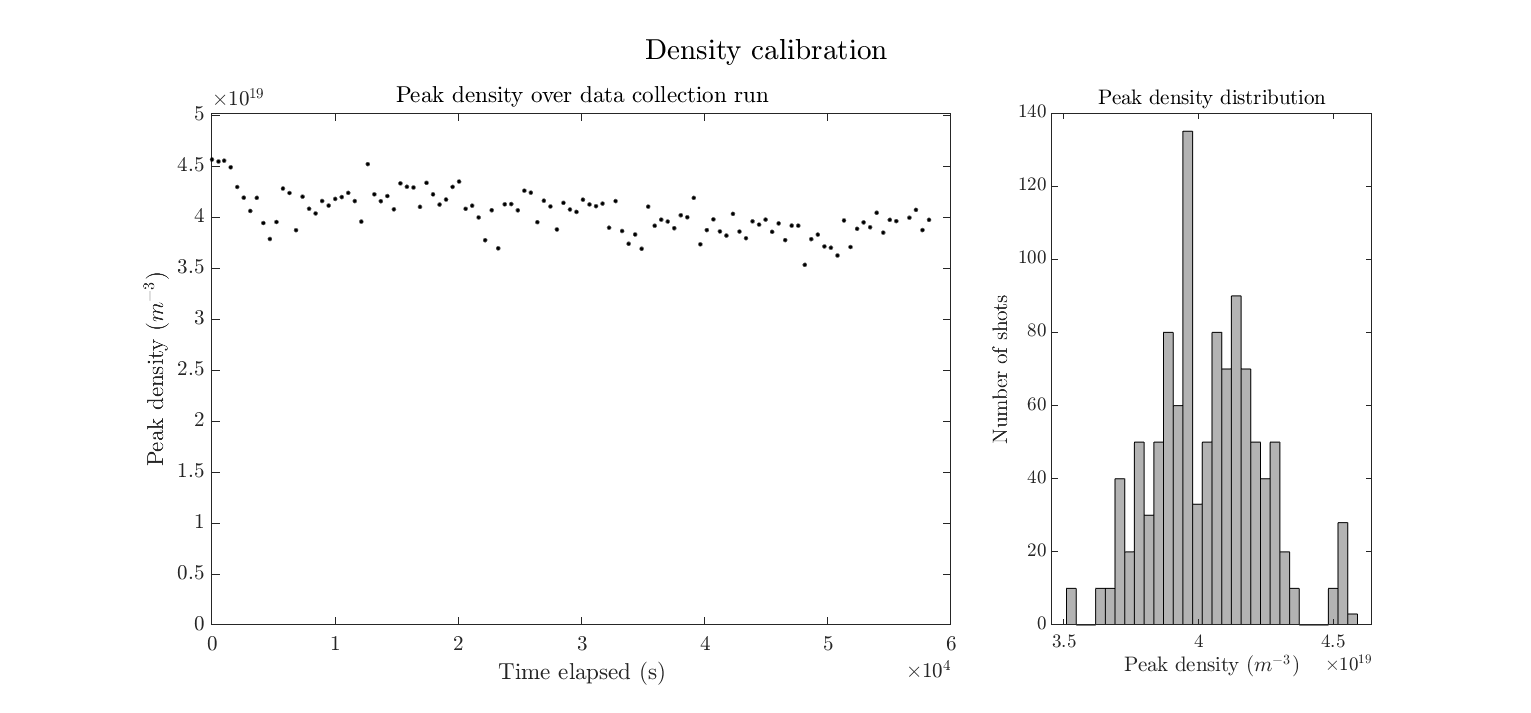
\includegraphics[width=\textwidth]{fig/QD/main/calibrate_QD_shots_01_stats.eps}
% %     \label{fig:qd-n0_by_time}
% %     \caption
% %     \title
% %     \end{figure}


% % \subsubsection{Dark counts}
% %     Even when the Helium source is not active, the MCP-DLD detector stack stil registers detection events.
% 	These may be genuine, spontaneous electron detection events seeded by background gas in the chamber or thermal excitation in the MCP, or indeed by transients in the DLD lines that are sufficient to trigger a digital pulse from the discriminator.
% 	These are referred to as \emph{dark counts}, by analogy to the Poissonian electronic noise in digital camera sensors like CMOS arrays.
% 	Indeed, the detector dark counts are uncorrelated events and so form a Poisson distribution \todo{Clarify \& graph of dark count statistics}.
% 	The correction for detector dark counts is entirely analogous to \emph{darkfielding} in precision photography, where images are taken without a light source to correct for detector noise.
% 	The spatial distribution of dark counts is shown in figure FIGURE, the time profile in figure PROFILES, and the calibration procedure is described in the next section.

    
% %     % average dark count rate of 5.6228 kHz/m$^2$.
% 	The evident structure in the dark count rate is accounted for in 

% %     The dark count rate is assumed to be uniform in time.
% 	It may be altered by high atomic fluxes of the condensate itself, but this is not a concern for the following reasons: One, we observe very similar thermal tails both above and below the condensate, suggesting that, at least, the quantum efficiency and dark count rates are not significantly different.
% 	Two, although there are some temporary hotspots on the detector during the peak BEC flux, these are only observed co-temporally with the falling BEC.
% 	The quantum depletion is detected far beyond the regions where this effect is noticable, and so they are not expected to contaminate the signal.

% %     A second source of background counts is the so-called \emph{trap leakage}, which is a measurable increase in the steady-state count rate while a BEC is held in the trap, which is visible in figure \ref{fig:qd-tof1}.
% 	Unlike the dark counts, the trap leakage has no obvious spatial structure.
% 	Correcting for these counts is therefore a matter of computing an average spurious count rate and then subtracting this from the detected count density, as described in the next section.
% 	Because the trap leakage stops when the trap is released, this correction is applied only to the leading side of the condensate.
    
% %     The best way to deal with it would be to extend the hold for ages, and then get heaps of statistics, but in the end I wound up using the 20-odd ms window of hold before drop in each case.
% 	This still gets to within ??? some margin of error when using all the data I have for a given run.
% 	In reality, the leak rate should depend on the BEC number, as, for instance, Majorana losses would induce an exponential decay of the trapped atom number, and Penning ionization losses scale with the squared density.
% 	There would also be density-dependent collision effects feeding the trap leak rate driven by changing the trapping frequencies, and different trap configurations would change the trap centre position, which could affect the detected density of the trap leakage.
% 	However, the count rates are so low that we do have the sensitivity to these effects, and so take a relatively simplistic treatment of the trap leakage, described in the next section.

% % \subsubsection{Transfer efficiency}

% %     The efficiency $\eta_0$ of the population transfer to the $m_J=0$ state is critical in determining the Tan contact, as the factor $1/\eta_0$ is the correction applied to the final signal in order to estimate the true signal density in the original condensate.
	

% %     The RF chirp transfers atoms into the $m_J = m$ states with efficiencies $\eta_m$.
% 	The chirp was adopted because, as described in \cite{Chang16}, it would minimize the momentum-dependence of the spin transfer pulse.
% 	The transfer efficiency cannot be calculated by counting the detected number in each cloud, as the condensates still saturate, leading to incorrect estimates.
% 	This is illustrated in figure SATCH-FRACTION.

% %     Instead, we can take advantage of the fact that the condensates have identical spatial profiles (to within a good approximation), albeit with different amplitudes, c.f.
% 	hydrodynamic expansion - density-dependent effects v small after 2ms?


% %     The momentum distribution of the thermal fraction of a degenerate Bose gas is known to be isotropic (see \cite{PitaevskiiStringariBook16} pp.
% 	160) and constitutes less than 5\% of the total population throughout this experiment.
% 	The momentum distribution of the thermal fraction takes the form

% %     \begin{equation}
% %         n_T(\textbf{k}) = \frac{1}{\lambda_T m \bar{\omega}}g_{3/2}\left(e^{-\beta (\hbar) k^2/2m}\right),
% %     \end{equation}

% %     which is manifestly invariant under rotations about the centre of momentum.
% 	Therefore, integrating over the $k_x$ and $k_y$ directions resolves the $k_z$-dependence of the momentum distribution.
% 	(You can talk through the physics better than this matey).
% 	After centering the clouds using a thresholding procedure described in the \textbf{Depletion} section, the time-of-flight profile of each cloud is divided pointwise by the sum of all the time-of-flight profiles.
% 	In the regions where the detector is unsaturated, the ratios $n_m(\textbf{k})/n(\textbf{k})$, where $n_m(\textbf{k})$ and $n(\textbf{k})$ are the momentum-space density of the $m_J=m$ clouds and the original BEC, respectively, are estimates of the transfer efficiency $\eta_m$, as shown in figure \href{fig:qd-fraction_calibration}.
% 	This figure also shows that detector saturation is not apparent in the thermal fraction of the trailing side of the BEC, and therefore suggests that saturation would be negligible in the depleted wings in the trailing edge.
% 	Further, the uniformity of the determined ratio across the thermal fraction is evidence that the RF transfer efficiency is independent of the particle momentum.

% %     \begin{figure}
% %     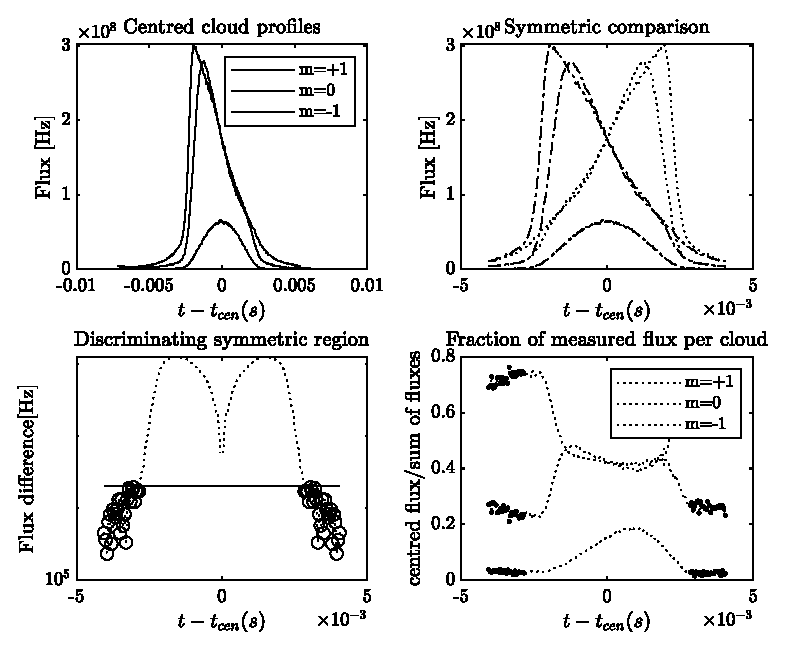
\includegraphics[width=\textwidth]{fig/QD/main/frac_cal.eps}
% %     \label{fig:qd-fraction_calibration}
% %     \caption
% %     \title
% %     \end{figure}

    

% % \subsubsection{Spin-mixing}

% %     In the depletion detection shots, we have observed a remaining presence of $mJ=1$ atoms.
% 	These are visible in figure PROFILES, as the step-up in flux rate at 0.56s in a) and the peak in detector flux at 0.55s in b).
% 	The cause of which is unclear but is suspected to be due to a collision process with a feature inside the chamber, as illustrated in figure CLOUDSMASH.
% 	Regardless of the cause, we calibrate for this contamination (also called \textit{spin mixing}).
% 	by running the depletion measurement without the RF transfer, instead measuring the time-of-flight profile of the $m_J=1$ cloud.
% 	After subtracting the background rates as appropriate, this provides a suitable calibration image for the spurious counts, which is subtracted from the measurement profiles, weighted by the transfer efficiency $\eta_1$.

% %     The count density of the $mJ=1$ states depends on the trapping frequencies, as shown by the clear difference between their contributions to figure PROFILES a) and b).
% 	This is likely because the trap centre and BEC width shifts with changing trap frequencies, so the push coil sequence would, left unchanged, result in different spray patterns on the detector.
% 	Unfortunately, we cannot rule out the presence of $mJ=-1$ counts on the detector without additional calibration (for example, taking yet another shot with a different RF transfer fraction).
% 	However, as the $m_J=-1$ clouds are determined to have about one tenth of the total atom population, and the $m_J=+1$ counts are suppressed by nearly three orders of magnitude by the push coils, if we assume a similar suppression of the $m_J=-1$ cloud then \todo{Worst-case bias of -1 counts}


    


% % \section{Determination of the Tan constant}\label{ssec:qd-processing}


% % 	The fit to the depletion profile $\tilde{n_0(k)}$ is obtained by taking the weighted sum of the k-space images for the depletion, spin-mixing, and dark count rates:

% % 	\begin{equation}
% % 		\tilde{n}_0(k) \approx \frac{1}{\eta_0}\left(n_0(k) - \eta_1(n_1(k)-\delta(k))-\delta_k-\lambda(k)\right)
% % 	\end{equation}

% % 	To avoid detector hotspots and to ensure we only use angular bins which extend far enough in k-space to capture some depletion, we specify the spherical sample region $\{(r_k,\theta,\phi): 1E6<r_k<3E7,\theta_{range},\phi_{range}\}$.
% 	Averaging over the angular bins commutes with the image summation because they're all linear.
% 	This produces one-dimensional radial profiles, as shown in figure K-PROFILES.
% 	The depletion and the thermal tails are isotropic, but the BEC is not, so the BEC peak is not physically representative.
% 	Or, remove it from the plot so it's just thermal - i.e.
% 	plot from the largest TF momentum.
	
    

% %     As in \cite{Chang16} we find the large-$\textbf{k}$ momentum distribution is isotropic, unlike the in-trap mean-field interactions, and conclude that the extreme momenta are not strongly affected by the mean-field.
% %     A typical condensate profile shown in Fig.
% 	\ref{k_profile}.
% 	Structure is visible over five orders of magnitude in density, comprised of the condensed, thermal, and depleted fraction before the signal drops below the dark-count background noise.
% 	There is some saturation evident around the low momentum values due to the high atom flux during BEC impact, however this part of the histogram is not used for the analysis.

% %     The Tan contact parameter is extracted by a fit to BEC density profile after subtracting the calibrated noise profiles.
% 	The functional form
% % 	$$
% %     n_{fit}(k) = \frac{N_{th}g_{3/2}exp(-k^2 \lambda_{dB} ^2 /4\pi)}{1.202(2\pi/\lambda_{dB})^3} + \frac{C}{(2\pi)^3 k^4} + const,
% %     $$

% %     includes contributions from the thermal fraction and depleted fraction and includes the free parameters $N_{th}$ the number of thermal atoms, $\lambda_{dB} = h/\sqrt{2\pi m k_B T}$ the thermal de Brogliewavelength, $const$ a constant to account for the detector background count rate, and $C$ is the scale of the fitted power law assumed to correspond to the Tan contact parameter.
% 	In the local density approximation, $C \approx C_{LDA} = \int d\textbf{r} [16\pi^2 \rho^2(\textbf{r},t)a^2]$, where $a$ is the scattering length and $\rho$ the atomic density.
% 	The initial guess for the fit constant $C$ is set to Tan constant predicted by the peak density and number calibrations.
% 	The initial temperatures are set manually for each directory.
% 	The thermal and the depleted parts of the profile are fitted individually to better constrain fitting parameters, and then a joint function is fitted to find the best overall parametrization.
	
    
% %     We verified the fitting method by analysing a test data set of known parameters, which was generated by the Metropolis-Hastings algorithm, and find the method recovers the test set parameters within a factor less than our experimental uncertainties.
    
% % \subsection{Verifying the method}
    
% %     Reliably estimating the parameters of a power-law distribution is nontrivial\cite{Clauset09}, and the robustness of the fitting method above has not been exhaustively tested.
% 	The LDA prediction is essentially that the single-particle wavefunctions, hence the single-particle probability distribution over momentum, are affected by many-body effects.
% 	One computes the single-particle probability density by dividing the condensate density by the number of particles (hence the $N_0$ term in the LDA), and then the problem of extracting the contact parameter from the data is an exercise in statistical parameter estimation.
% 	As shown by Clauset et al \cite{Clauset09}, fitting these functions tends to produce incorrect estimates of parameters.
% 	The method outlined in Clauset was proven to asymptotically converge with probability 1 to the correct fit parameters of a power law distribution, but would need to be extended to derive a maximum likelihood estimator for a power law overlaid on a constant background.

% % \section{Discussion}
% % \label{qd-discussion}

% % \subsection{Findings}
    
% %     According to theoretical predictions based on the local density approximation \cite{Chang16}, the contact constant $C_{LDA}$ of the depleted fraction should vary linearly with the peak condensate density $n_0$.
% 	This was found in previous experiments\cite{Chang16}, although their scaling factor greater by a factor of $\sim$6.5.
% 	In Fig.
% 	XX, we plot our measured values of $C$ and $n_0$ , identifying the fit parameter $C$ with the contact constant $C_{LDA}$ .
% 	A linear fit to the contact constant variation finds a gradient approximately 1.7 times more than the theory predicts.

% %     Our findings suggests that the visibility of the quantum depletion in the far-field momentum distribution is indeed a real physical effect.
% 	Our findings are corroborated by theoretical work.
% 	However, the question remains open as to why the observed population of the quantum depletion is greater than predicted by the otherwise successful Bogoliubov theory.
% 	Possible confounding factors:
% %     \begin{itemize}
% %     	\item Intra-cloud scattering
% %     	\item Trap switchoff or early-falltime dynamics,switch-off timescale may be relevant (compare \cite{Chang16} with \cite{Qu16}).
% %     	\item $m_J=-1$ counts
% %     \end{itemize}

% % 	We have assumed that the RF transfer is momentum-independent, but this could be violated by inhomogeneities or transients in the magnetic field.
% 	The RF pulse may increase the Penning ionization rate in the depolarized sample, even though the density is low, which would alter the momentum profile.
% 	While applying the magnetic separation pulse, the condensates may scatter off each other.


    


% % \subsection{Future work}
	
% %     A possible future experimental extension is to outcouple atoms using a broadened Raman transition.
% 	This would have the benefit of moving the outcoupled atoms through the cloud rapidly, minimising the effects of repulsive inter-atomic interactions that normally affect the outcoupled profiles.
% 	This should shed some light on whether interactions during trap switch off are the origin of the momentum tails.
% 	One could test the importance of particle scattering or Penning ionization by delaying the Rabi transfer to the $M_J = 0$ state, but this could increase vulnerability to stray magnetic fields.
% 	There is scope to optimize the RF transfer sequence to achieve much higher transfer efficiency for a stronger signal
    
    

    

